\clearpage
\section{Signal signature and base selection}
\label{sec:signal-signature}

To develop an effective analysis strategy, the signal kinematics are studied and exploited. The production and decay of electroweakinos give rise to unique event characteristics that can be leveraged to differentiate the signal from the \gls{sm} background. Distributions of key observables from signal and background processes are compared in order to define a preselection or set of base cuts that retains the maximum signal while rejecting as much background as possible. All the following distributions of key observables were generated by weighting the simulated data to the Run II luminosity of $\lumi = 135 \fbinv$ and requiring at least one jet in the event with $\pt \geq 30\GeV$ and $\abs{\eta}<2.4$. Discussion is provided for each event property, and the incorporation of additional selection criteria is specified building toward the base selection. 

\subsection{Missing transverse energy}
\label{subsec:signal-met-mht}

A driving factor for most searches for \gls{dam} at the LHC is the presence of a \gls{dam} candidate in the final state. The identity and properties of the particle (or particles in the case of multiple \gls{dam} candidates) vary, but they do have much in common. In this \gls{susy} search, the \gls{dam} candidate is the \gls{lsp}, assumed to be a \gls{neutralino}. A neutral particle that does not interact electromagnetically or via the strong force (\ie, is colorless) will not be detected and will leave traces in the form of a transverse momentum imbalance, which is referred to as \gls{met} (missing transverse energy or missing transverse momentum). Because of R-parity conservation, the signal contains two \gls{dam} candidates in the final state, which are the \glspl{lsp}, the \glspl{neutralino} \neuto. Therefore, a considerable magnitude of \gls{met} is expected in the signal. As described in Section~\ref{subsec:met}, a suitable proxy for the \gls{met} is the missing transverse hadronic energy, or \gls{mht}, which is highly correlated with \gls{met}, but better suited to the definition of lepton isolation and its use in the background estimation methods. Both $\MET$ and $\mht$ observables are examined in Figure~\ref{fig:signal-met-mht}.


\begin{figure}[!htb]
\centering
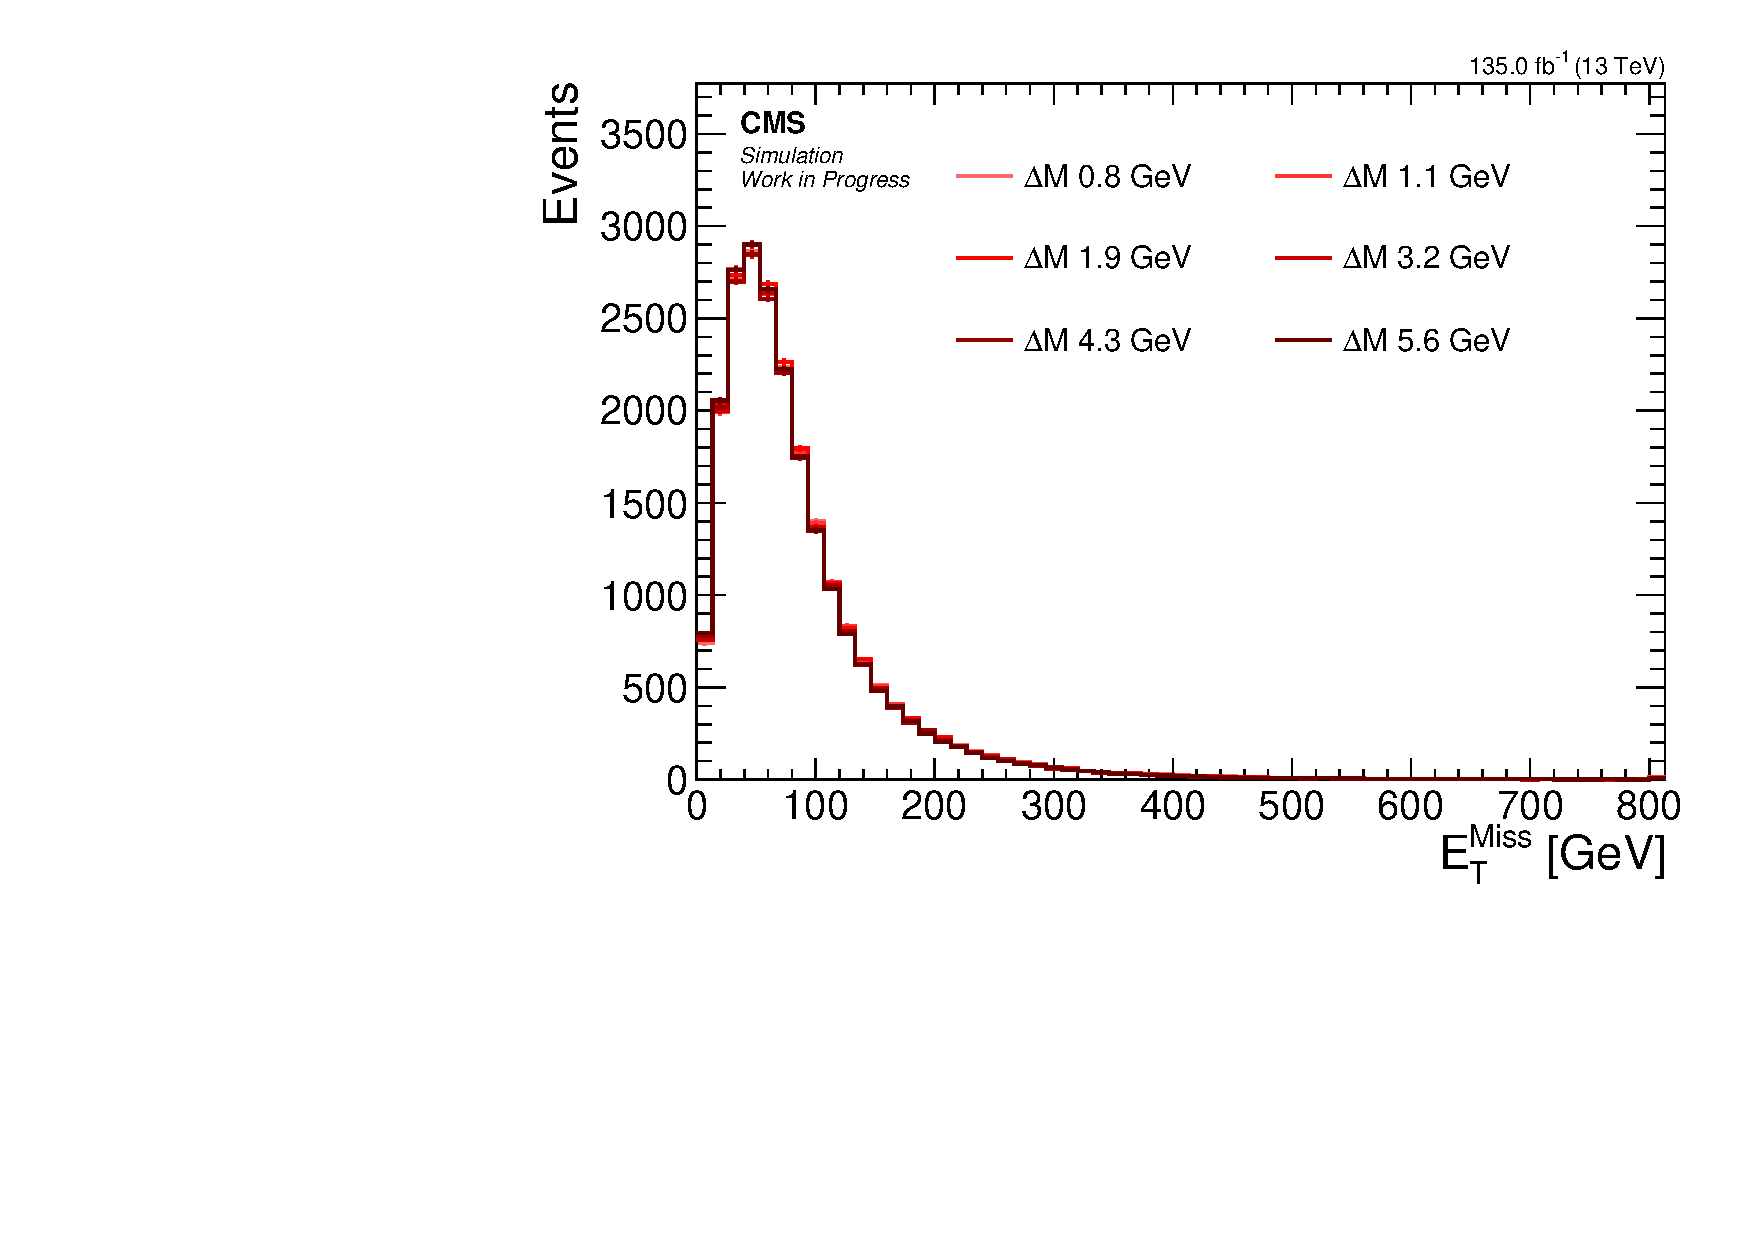
\includegraphics[width=0.48\linewidth]{plots/signal_common_distributions_fixed_mu/none_MET.pdf} \,
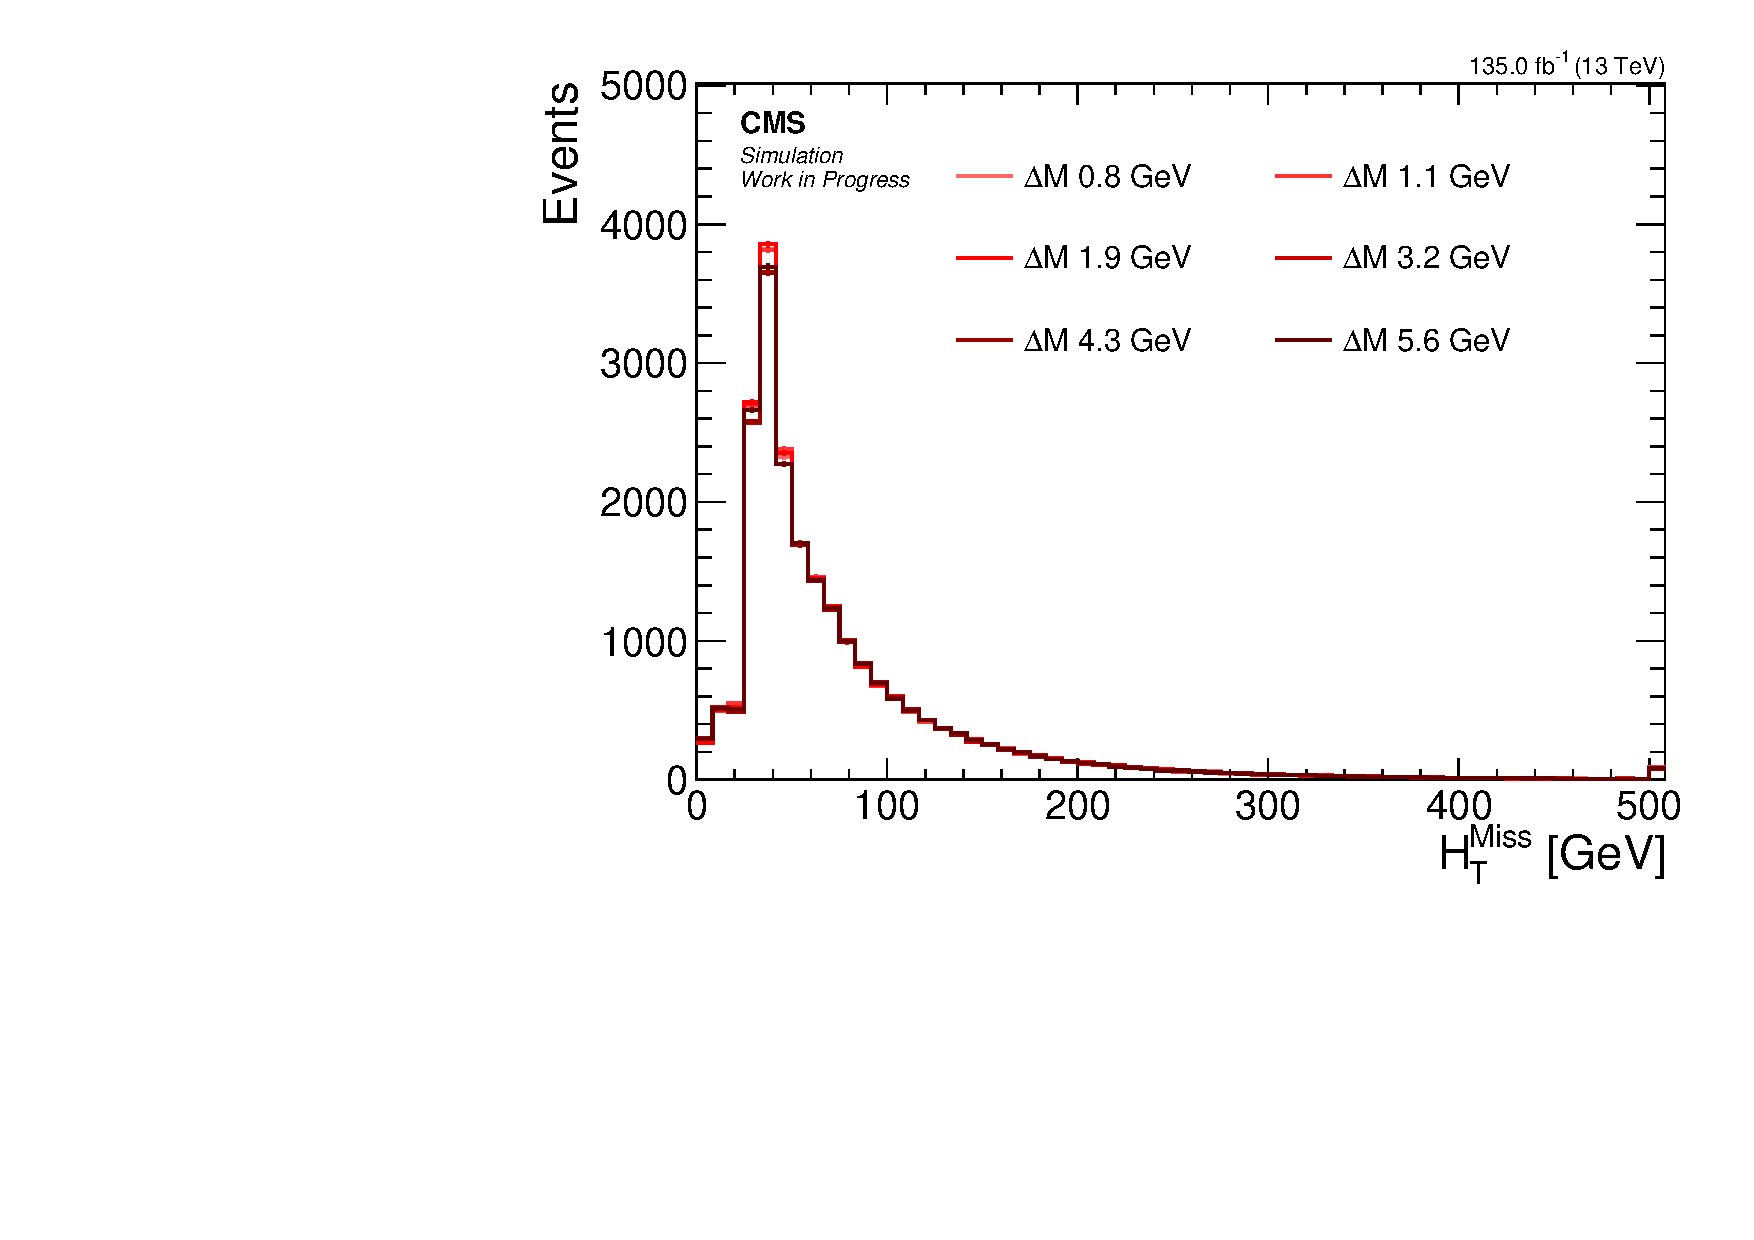
\includegraphics[width=0.48\linewidth]{plots/signal_common_distributions_fixed_mu/none_MHT.pdf}  \\
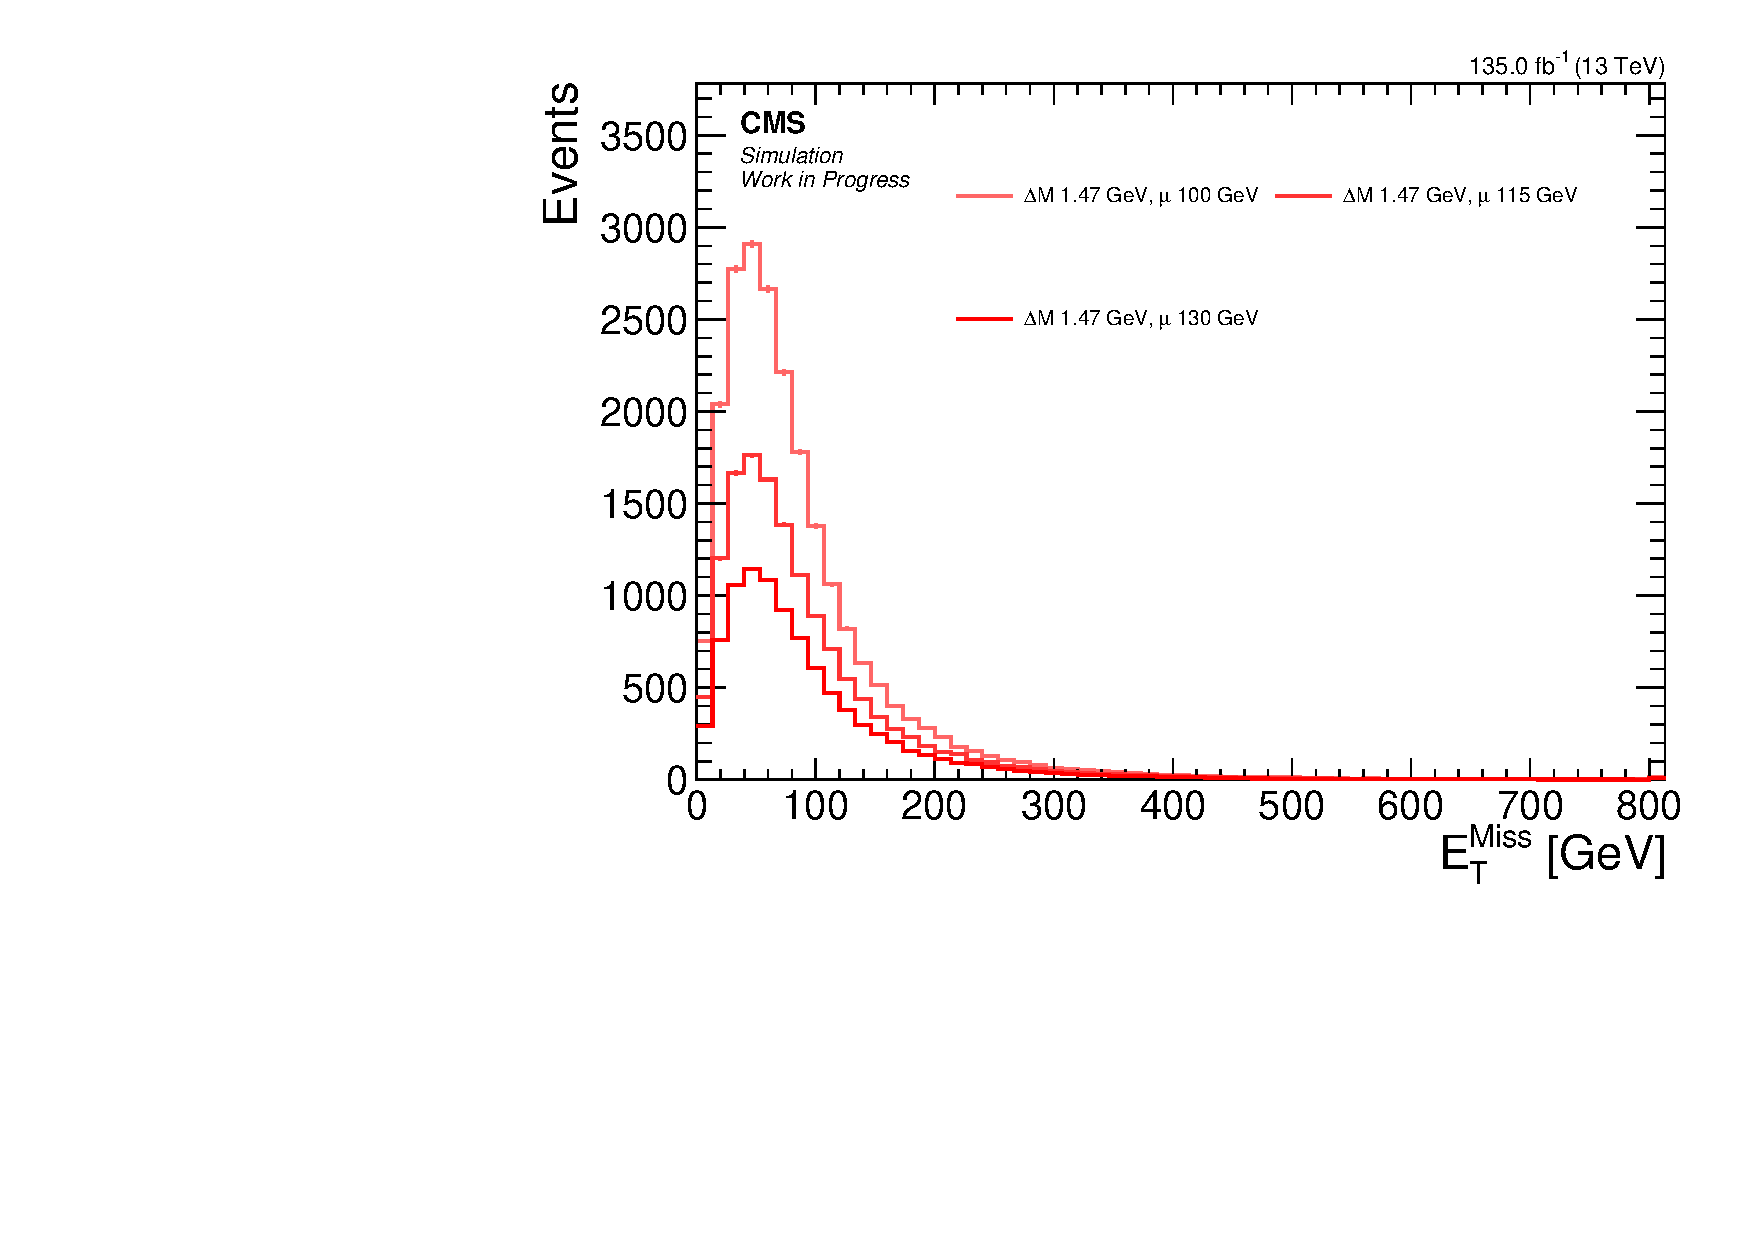
\includegraphics[width=0.48\linewidth]{plots/signal_common_distributions_fixed_dm/none_MET.pdf} \,
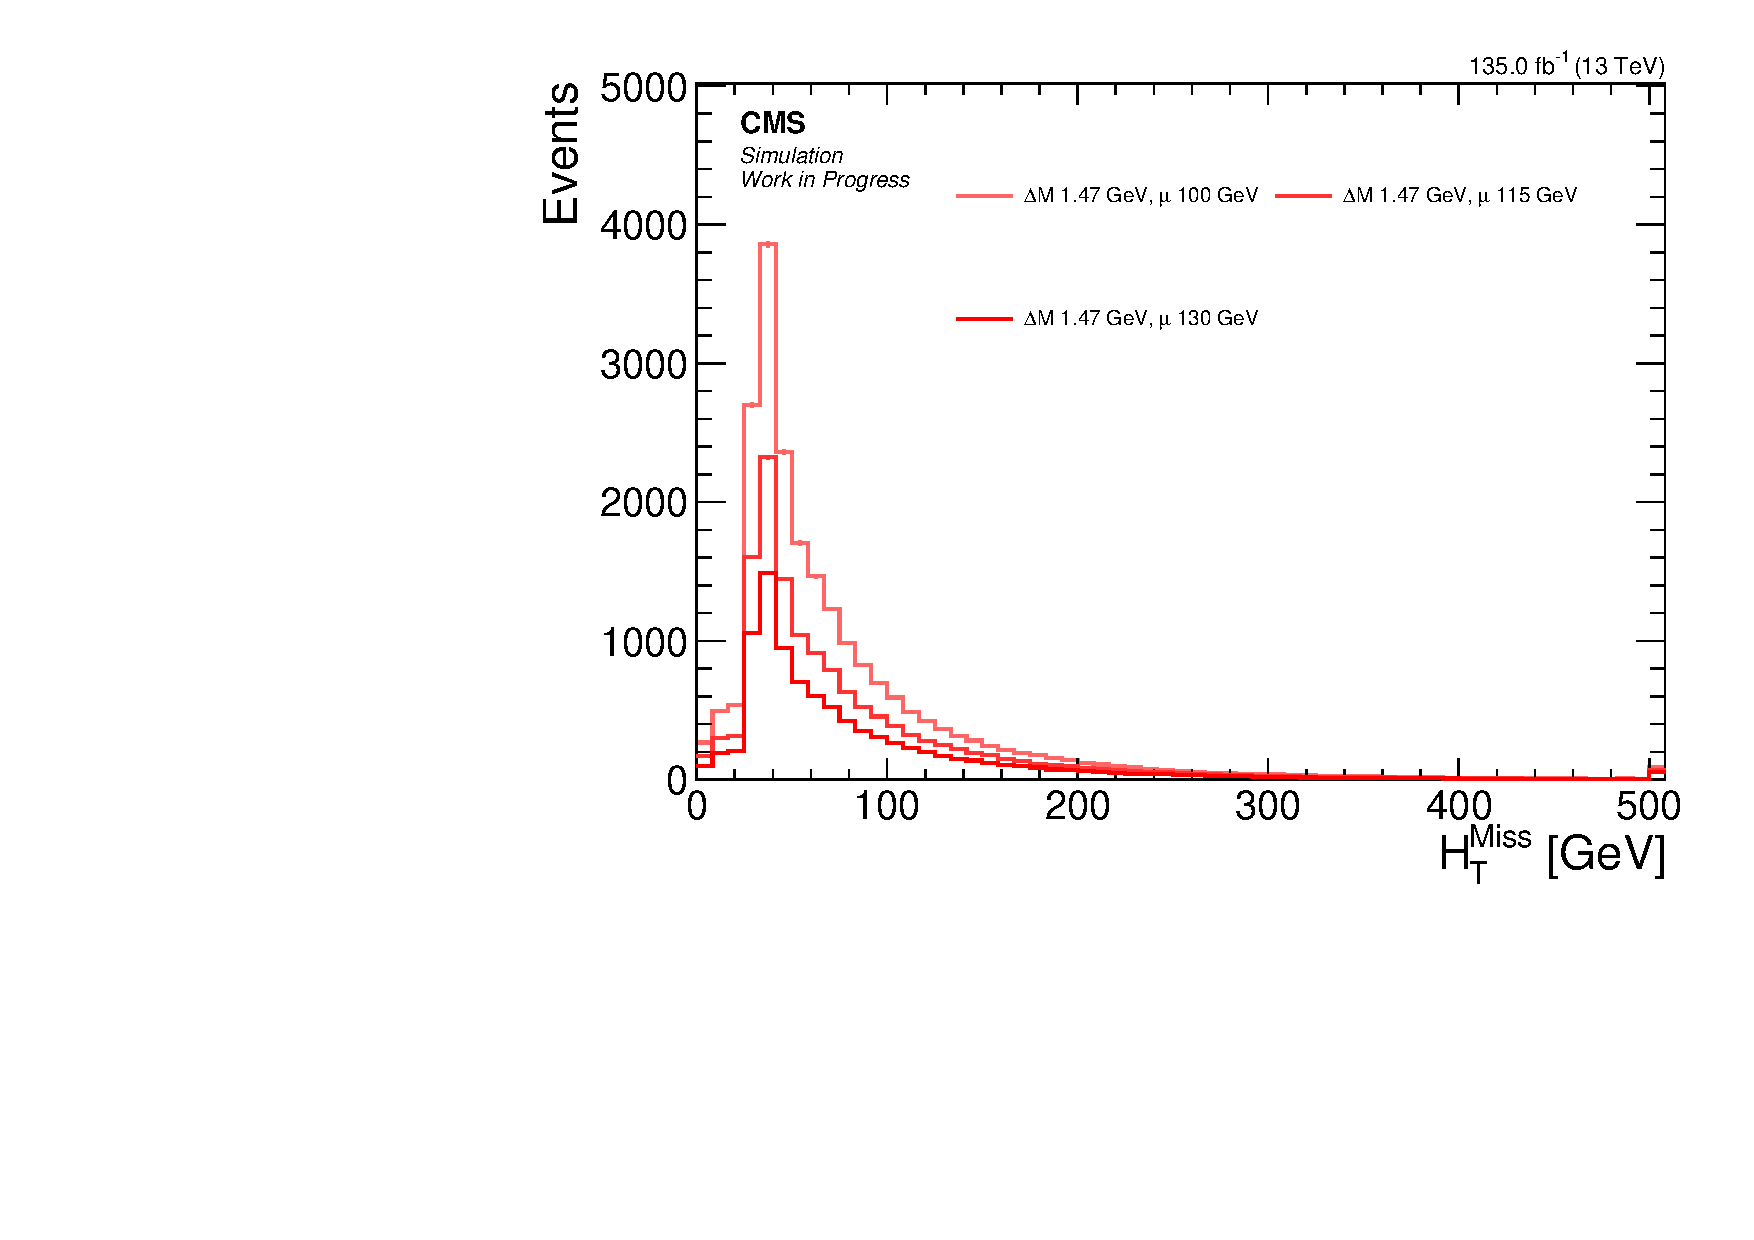
\includegraphics[width=0.48\linewidth]{plots/signal_common_distributions_fixed_dm/none_MHT.pdf}  \\
\caption[Signal $\MET$ and $\mht$ distributions]{ Signal distributions of \MET (left) and \mht (right) comparing various $\dm$ with a fixed higgsino parameter $\mu=100\GeV$ (upper), and comparing various $\mu$ with fixed $\dm=1.47\GeV$ (lower).}
\label{fig:signal-met-mht}
\end{figure}

As expected, $\MET$ and $\mht$ are largely unaffected by the different choices for \dm, while the higgsino parameter $\mu$ affects the distributions mainly through its falling production cross section as a function of the higgsino parameter $\mu$. The region of interest in order to be efficient with respect to the triggers is located at $\mht\geq 220\GeV$, as discussed in Section~\ref{sec:trigger}. Although this is a harsh and inefficient cut, it becomes apparent when examining the \gls{sm} background in both regions of $\mht < 220\GeV$ and $\mht\geq 220\GeV$ to conclude that most of the sensitivity comes from the $\mht\geq 220\GeV$ region, as the production of real \gls{mht} (or \gls{met}) results from the production of neutrinos in the event. These are much less common than \gls{qcd} events that dominate the $\mht < 220\GeV$ region.

\subsection{Jets and hardronic activity}

As mentioned in the previous section, signal events tend to have small momentum imbalance. In order to induce significant missing transverse energy, some additional activity must take place within the events, and this most often comes in the form of one or more \glsreset{isr}\gls{isr} jets. An \gls{isr} jet is created when one of the incoming protons emits radiation (such as a quark or a gluon) before the interaction. If a jet with sufficiently high \gls{pt} is emitted, the remainder of the interaction is recoiled against this jet and imparts momentum onto the system of invisible particles in the opposite direction. As a result, the boosted \glspl{neutralino} \neuto give rise to higher \gls{mht}. As described in Section~\ref{subsec:jets}, the jets are required to have $\pt \geq 30\GeV$ and be located within the tracker acceptance $\left(\abs{\eta}<2.4\right)$. At least one such jet is required in each event. The distributions of the number of jets and the leading jet \pt are displayed in Figure~\ref{fig:signal-njets-ljpt}.

\begin{figure}[!htb]
\centering
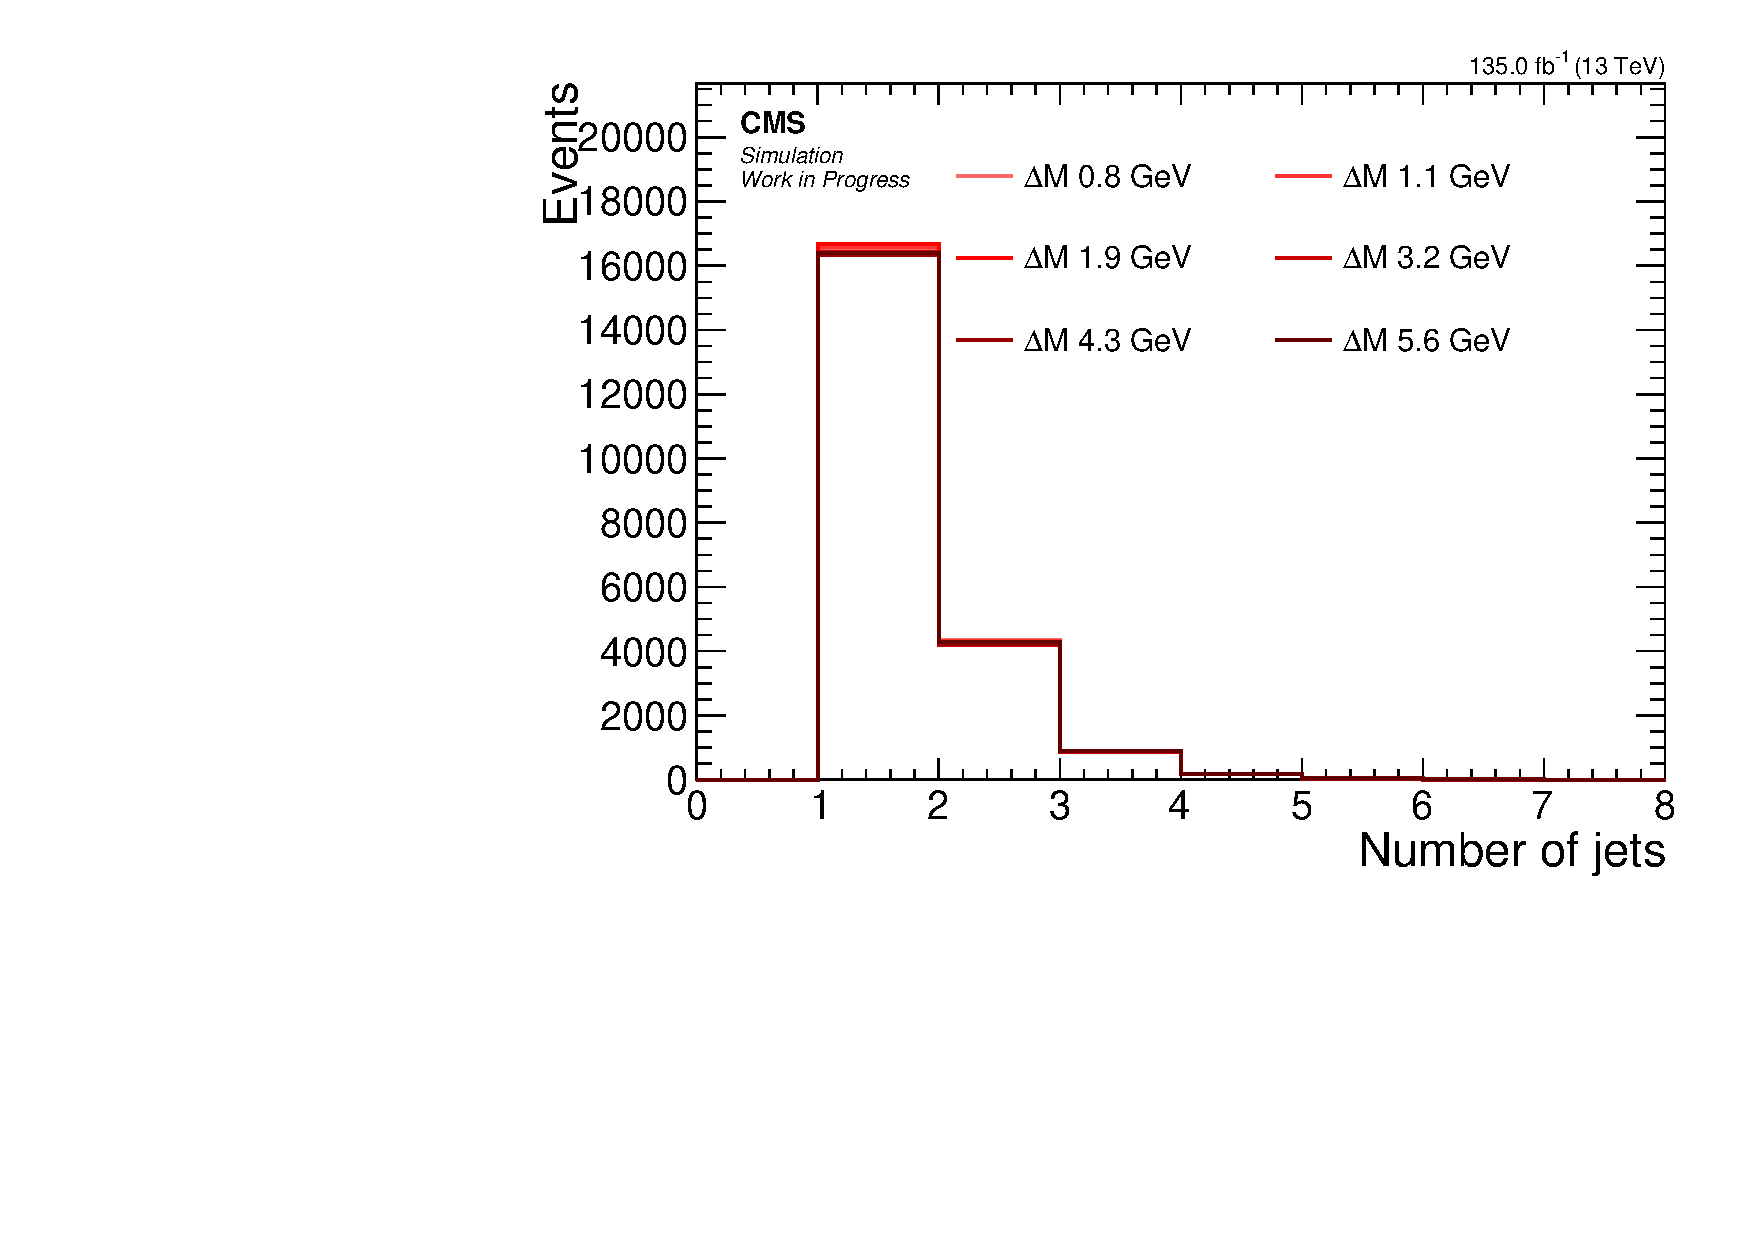
\includegraphics[width=0.48\linewidth]{plots/signal_common_distributions_fixed_mu/none_NJets.pdf} \,
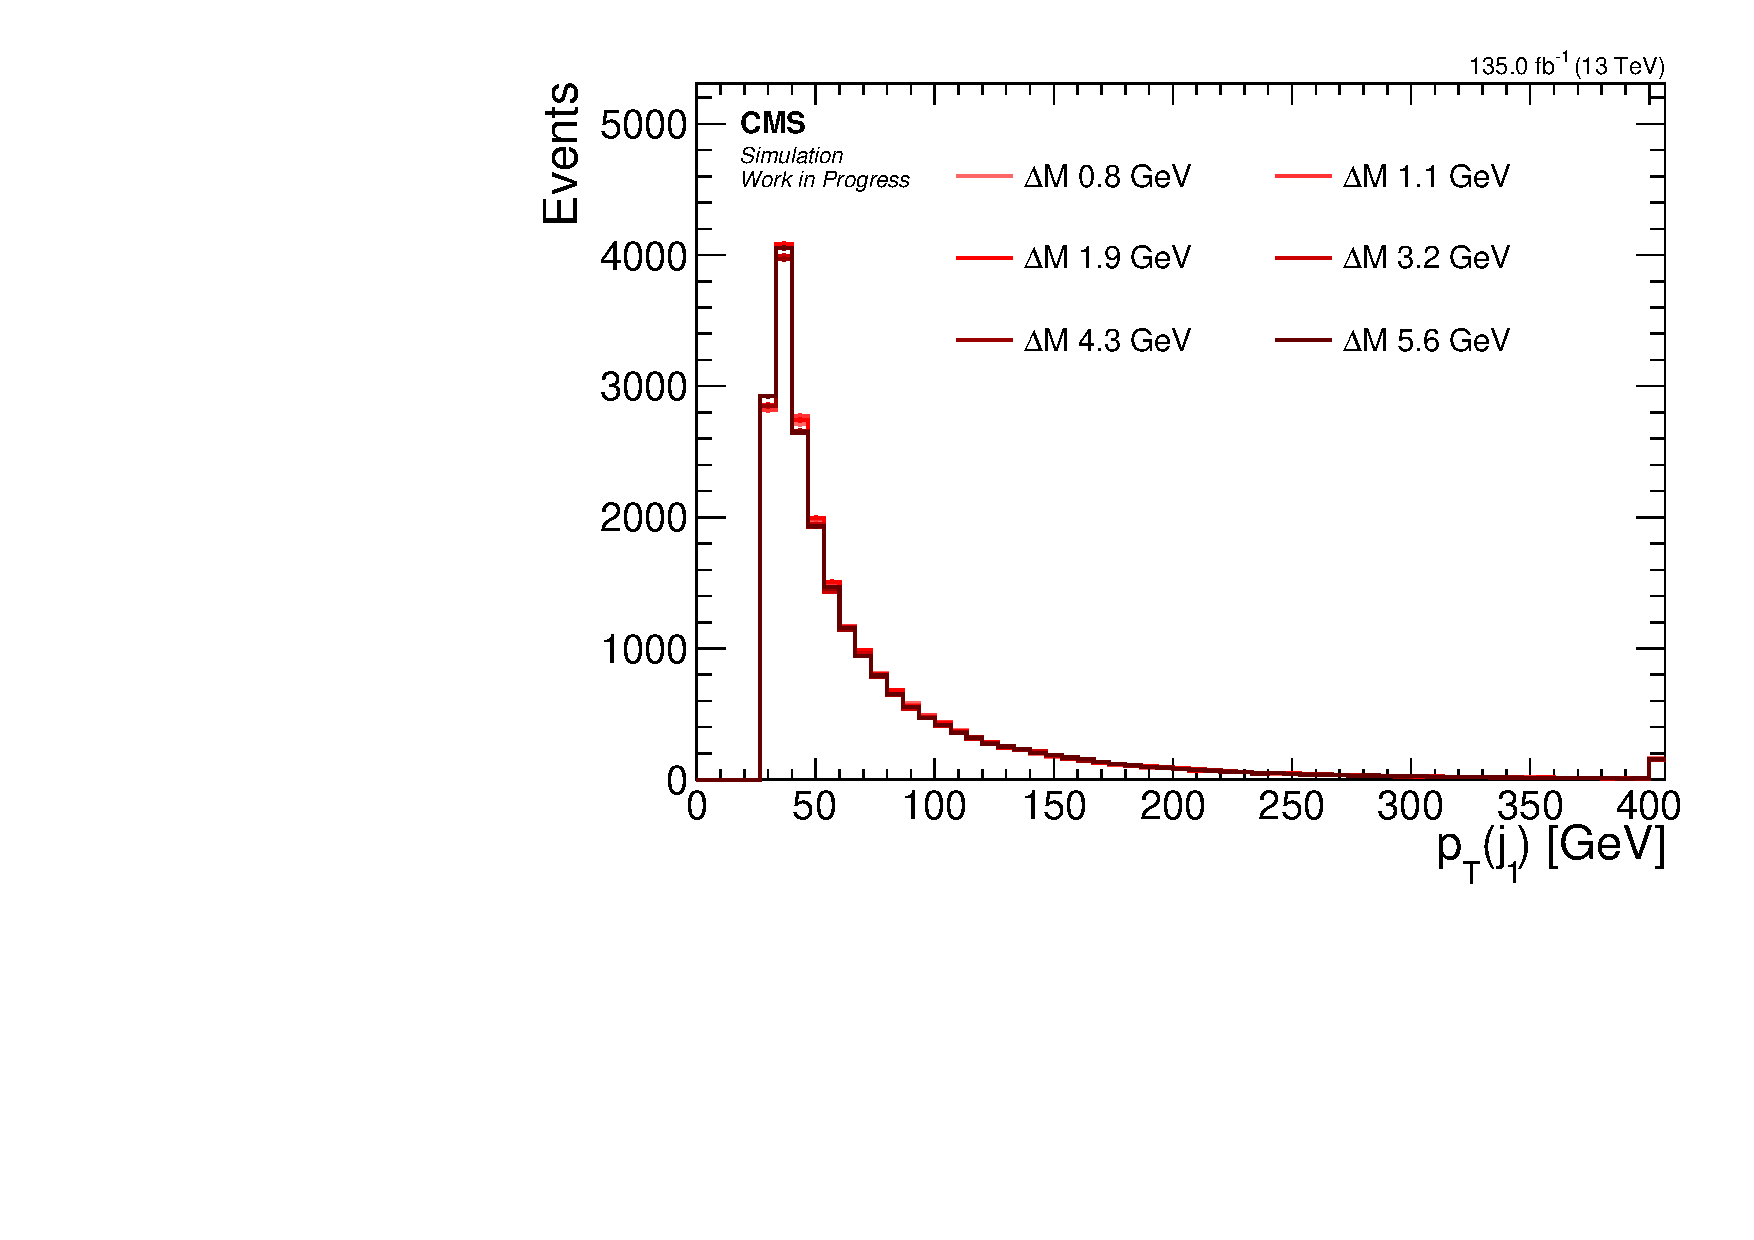
\includegraphics[width=0.48\linewidth]{plots/signal_common_distributions_fixed_mu/none_LeadingJetPt.pdf}  \\
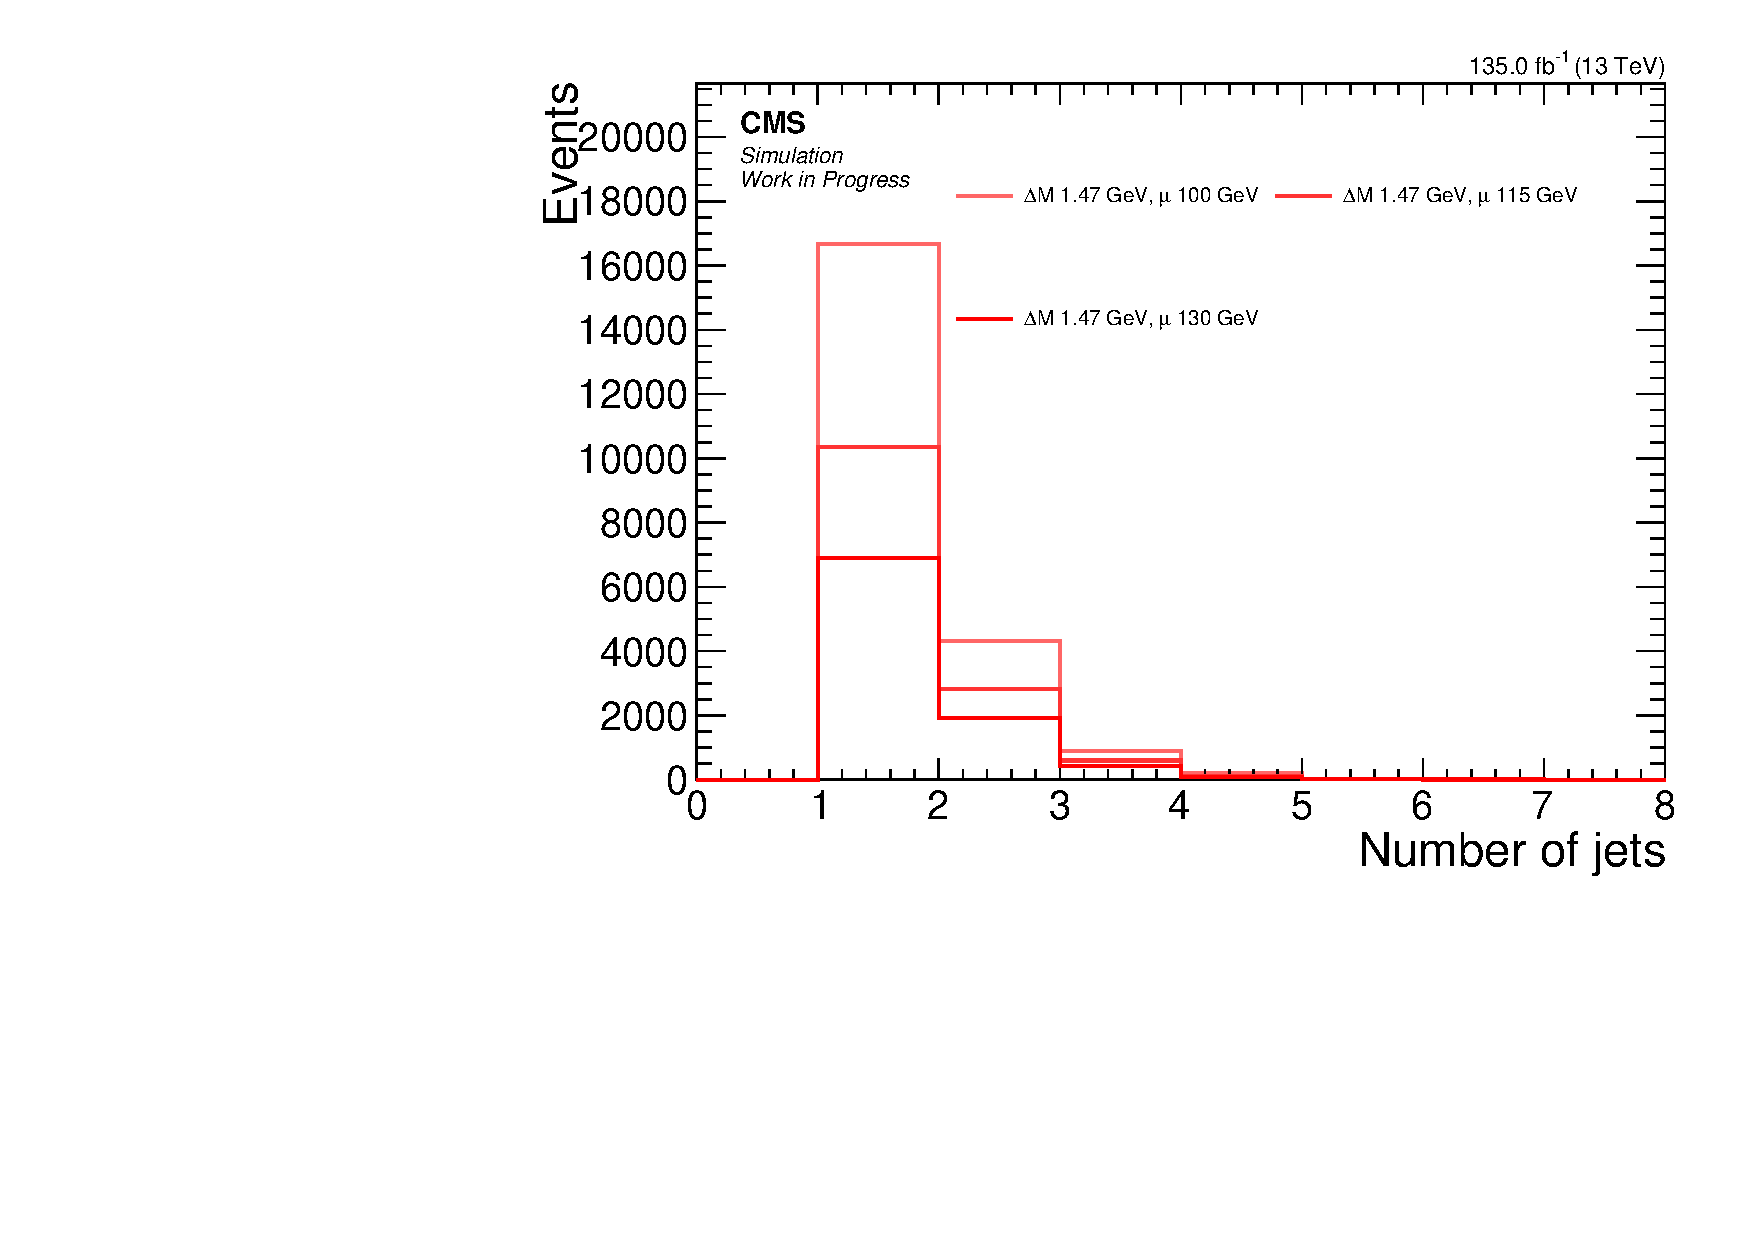
\includegraphics[width=0.48\linewidth]{plots/signal_common_distributions_fixed_dm/none_NJets.pdf} \,
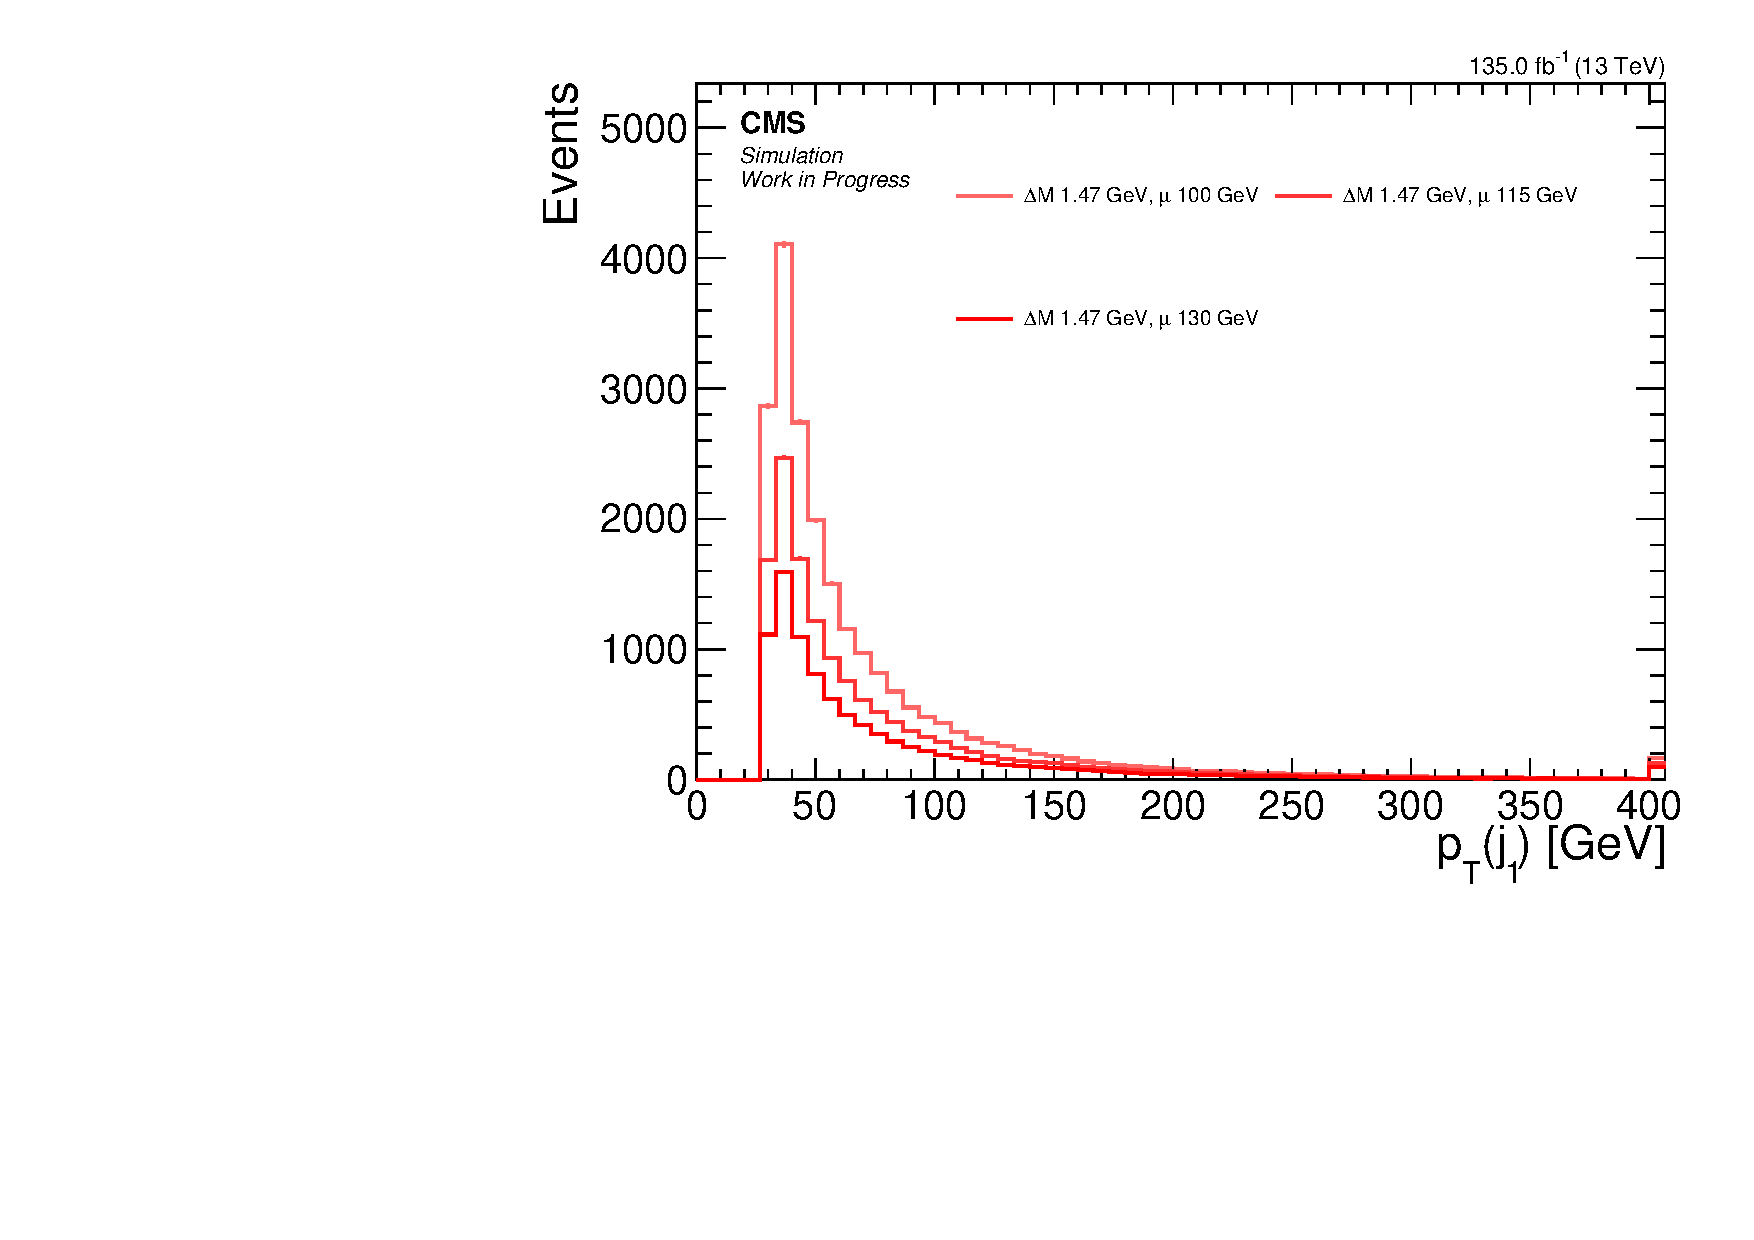
\includegraphics[width=0.48\linewidth]{plots/signal_common_distributions_fixed_dm/none_LeadingJetPt.pdf}  \\
\caption[Signal \emph{number of jets} and \emph{leading jet \pt} distributions]{ Signal distributions of \emph{number of jets} (left) and \emph{leading jet \pt} (right) comparing various $\dm$ with a fixed higgsino parameter $\mu=100\GeV$ (upper), and comparing various $\mu$ with fixed $\dm=1.47\GeV$ (lower).}
\label{fig:signal-njets-ljpt}
\end{figure}

The signal signature rarely includes a \PQb-jet, that is, a jet resulting from the hadronization of a bottom quark. However, standard model top quark pair production leads to a large numbers of events with significant missing transverse energy and two or more \PQb-jets. To reject this background, events are vetoed if a \PQb-jet is identified in the event. As described in Section~\ref{subsec:jets}, the \DEEPCSV bottom flavor tagging discriminant with a medium working point is used. The multiplicity of \PQb-tagged jets is shown in Figure \ref{fig:signal-bjets}, where the choice of number of \PQb-tagged jets equals to zero appears well-justified. 

\begin{figure}[!htb]
\centering
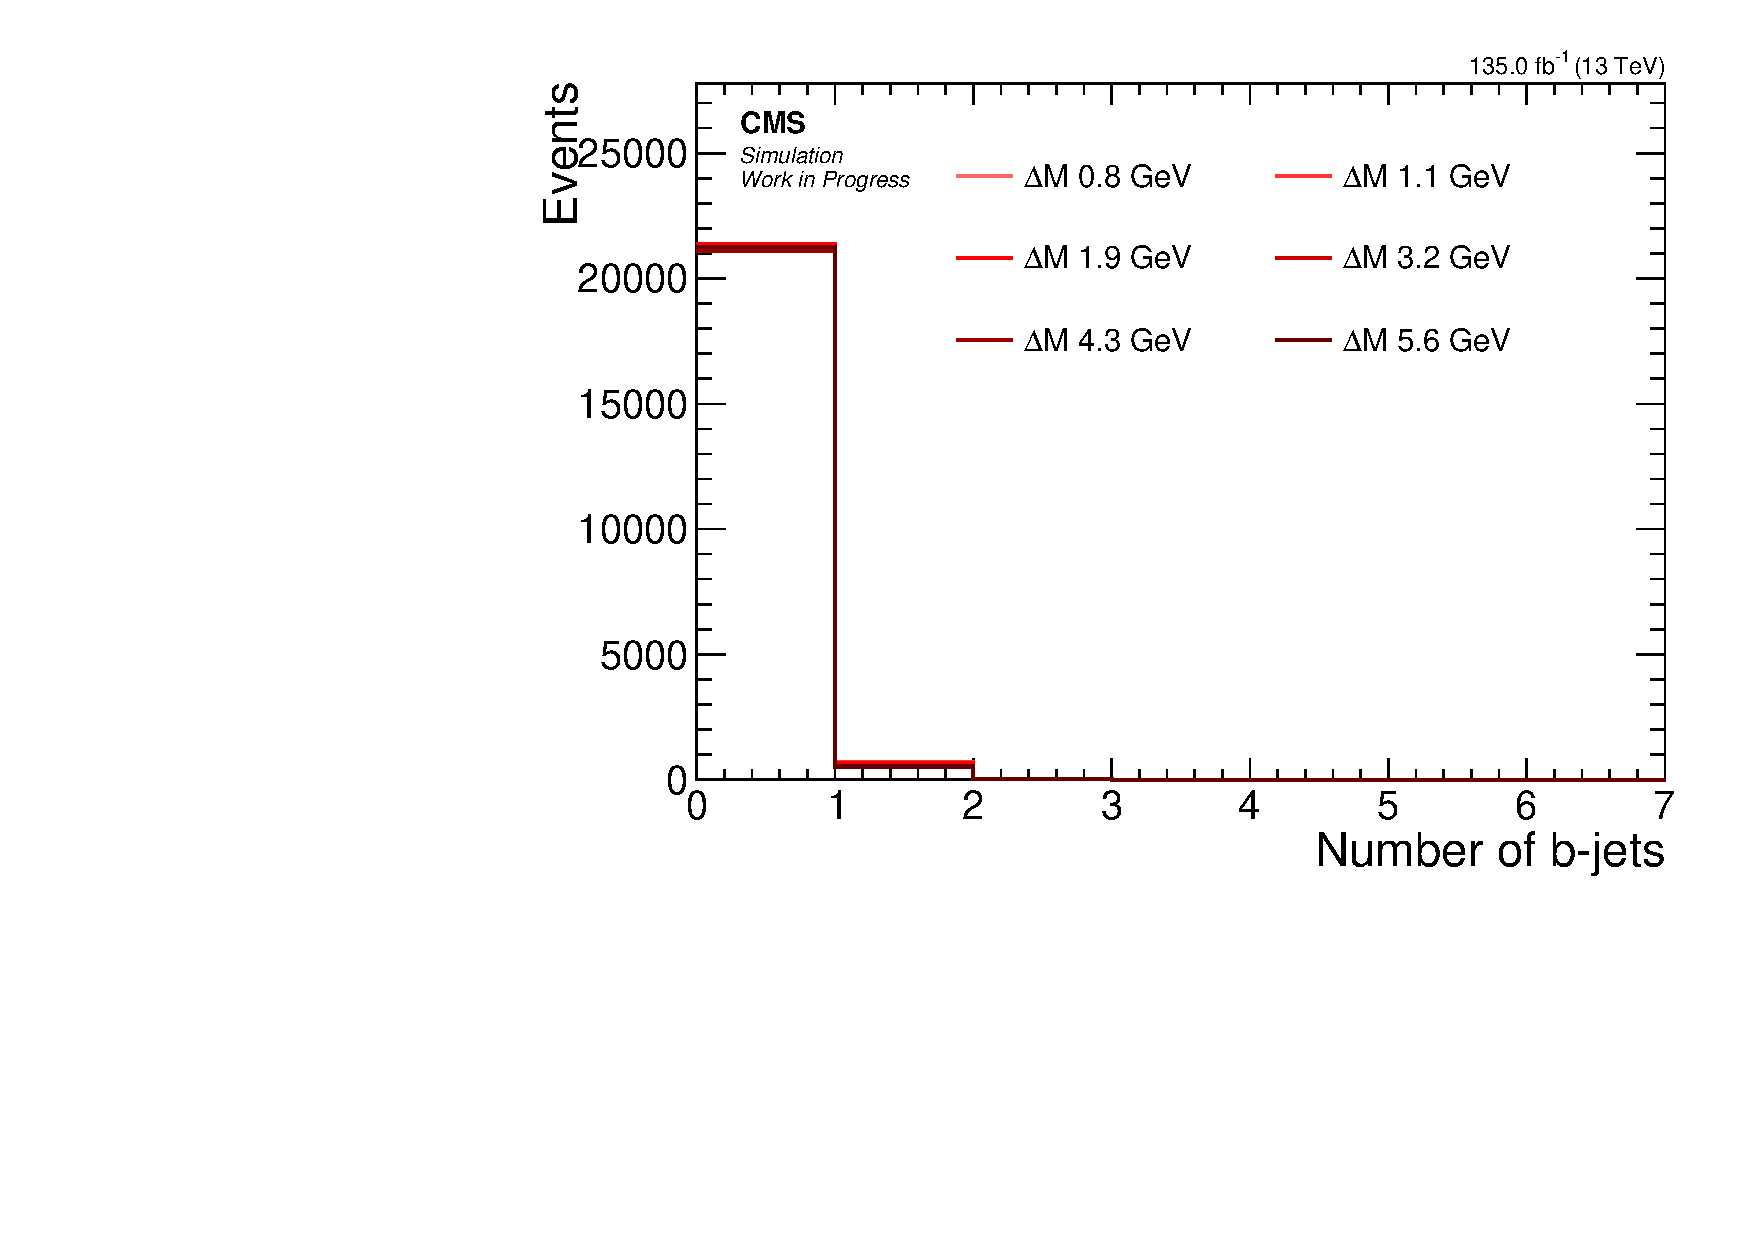
\includegraphics[width=0.48\linewidth]{plots/signal_common_distributions_fixed_mu/none_BTagsDeepMedium.pdf} \,
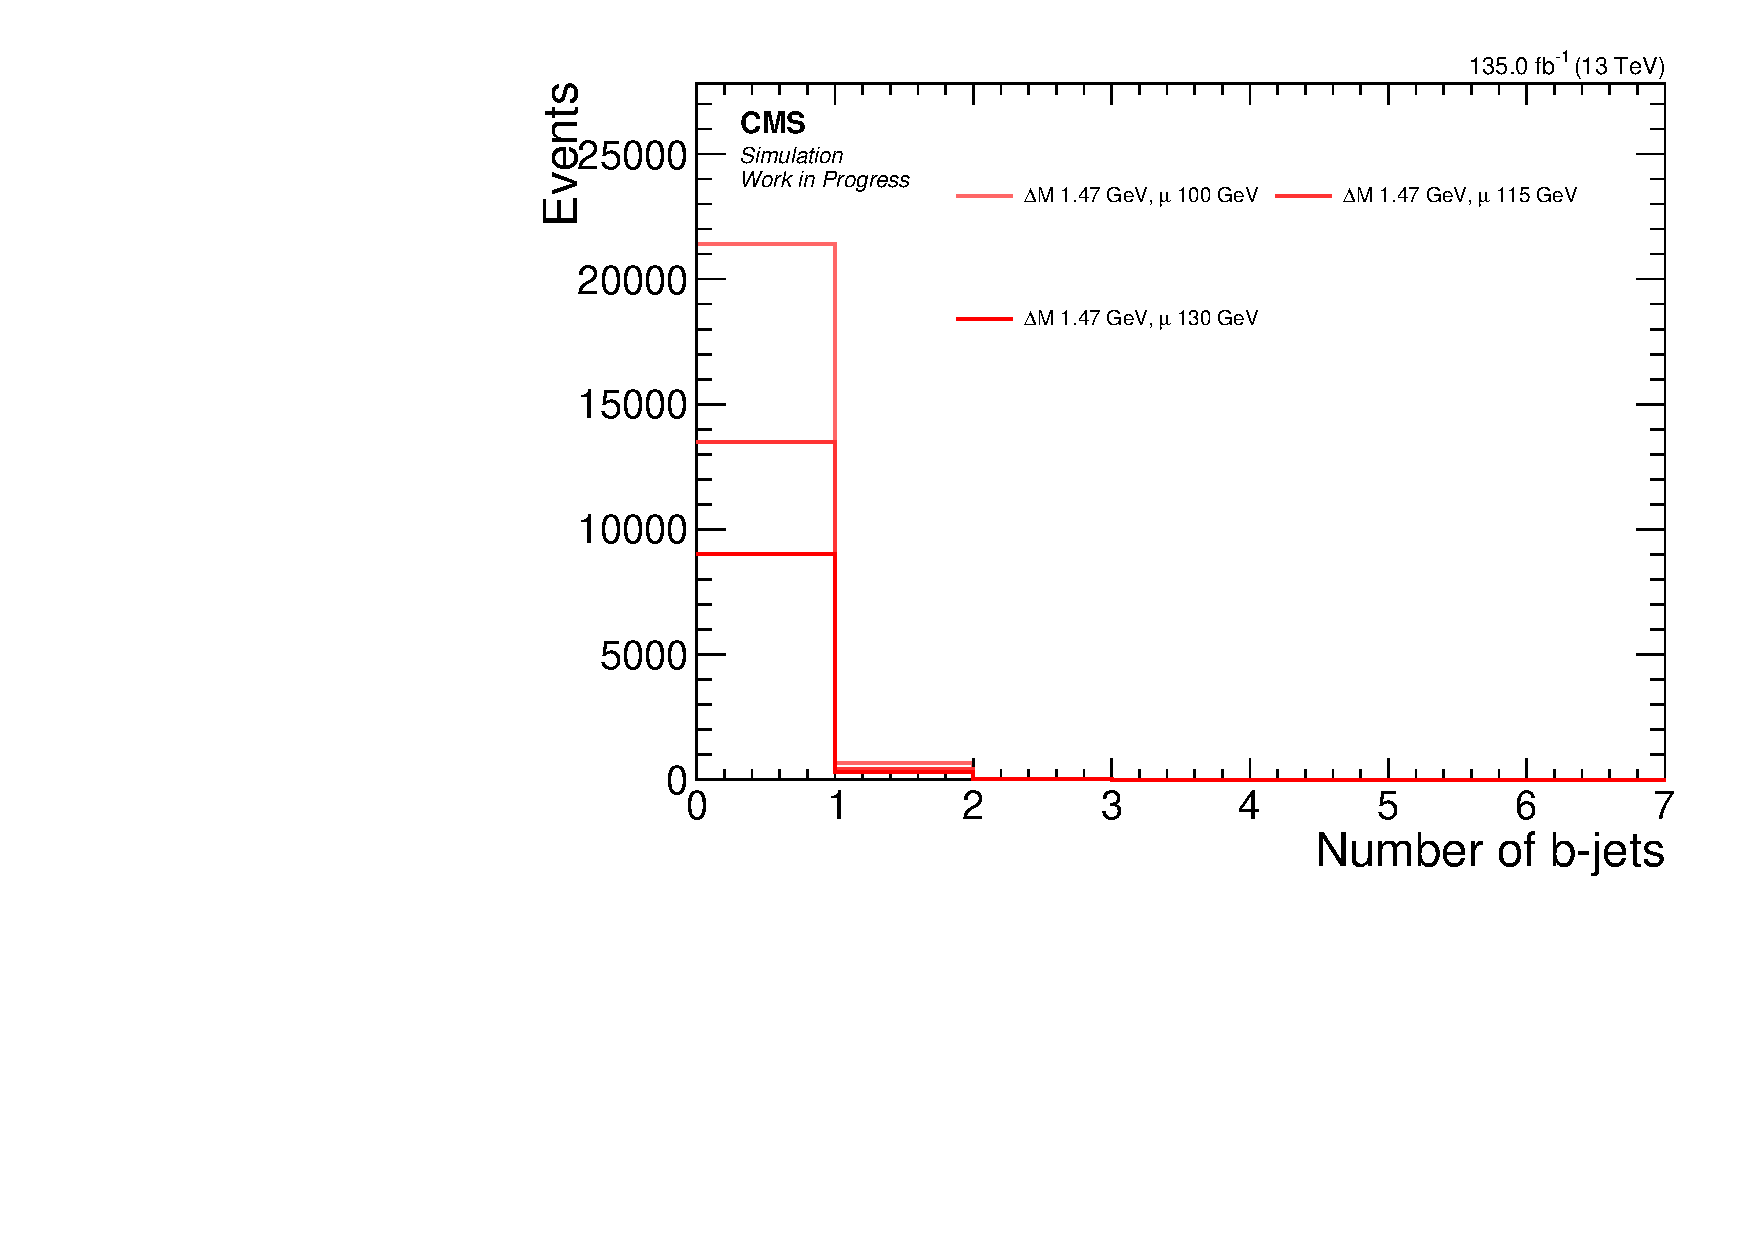
\includegraphics[width=0.48\linewidth]{plots/signal_common_distributions_fixed_dm/none_BTagsDeepMedium.pdf}  \\
\caption[Signal \emph{number of b-tagged jets} distributions]{ Signal distributions of \emph{number of b-tagged jets} comparing various $\dm$ with a fixed higgsino parameter $\mu=100\GeV$ (left), and comparing various $\mu$ with fixed $\dm=1.47\GeV$ (right).}
\label{fig:signal-bjets}
\end{figure}

As an \gls{isr} jet is required in the event, it is expected that the \gls{met} and the \gls{mht} will be directed in the opposite direction of the jet, or at an asimuthal angle close to $\pi$. This feature is not as clearly observed in events with multiple jets in the \gls{sm} background, such as those arising from \gls{qcd}, where the missing transverse energy tends to align with the leading or sub-leading jet. To reduce the \gls{qcd} background, a requirement of $\mindphimhtjets > 0.4$ is imposed.

\begin{figure}[!htb]
\centering
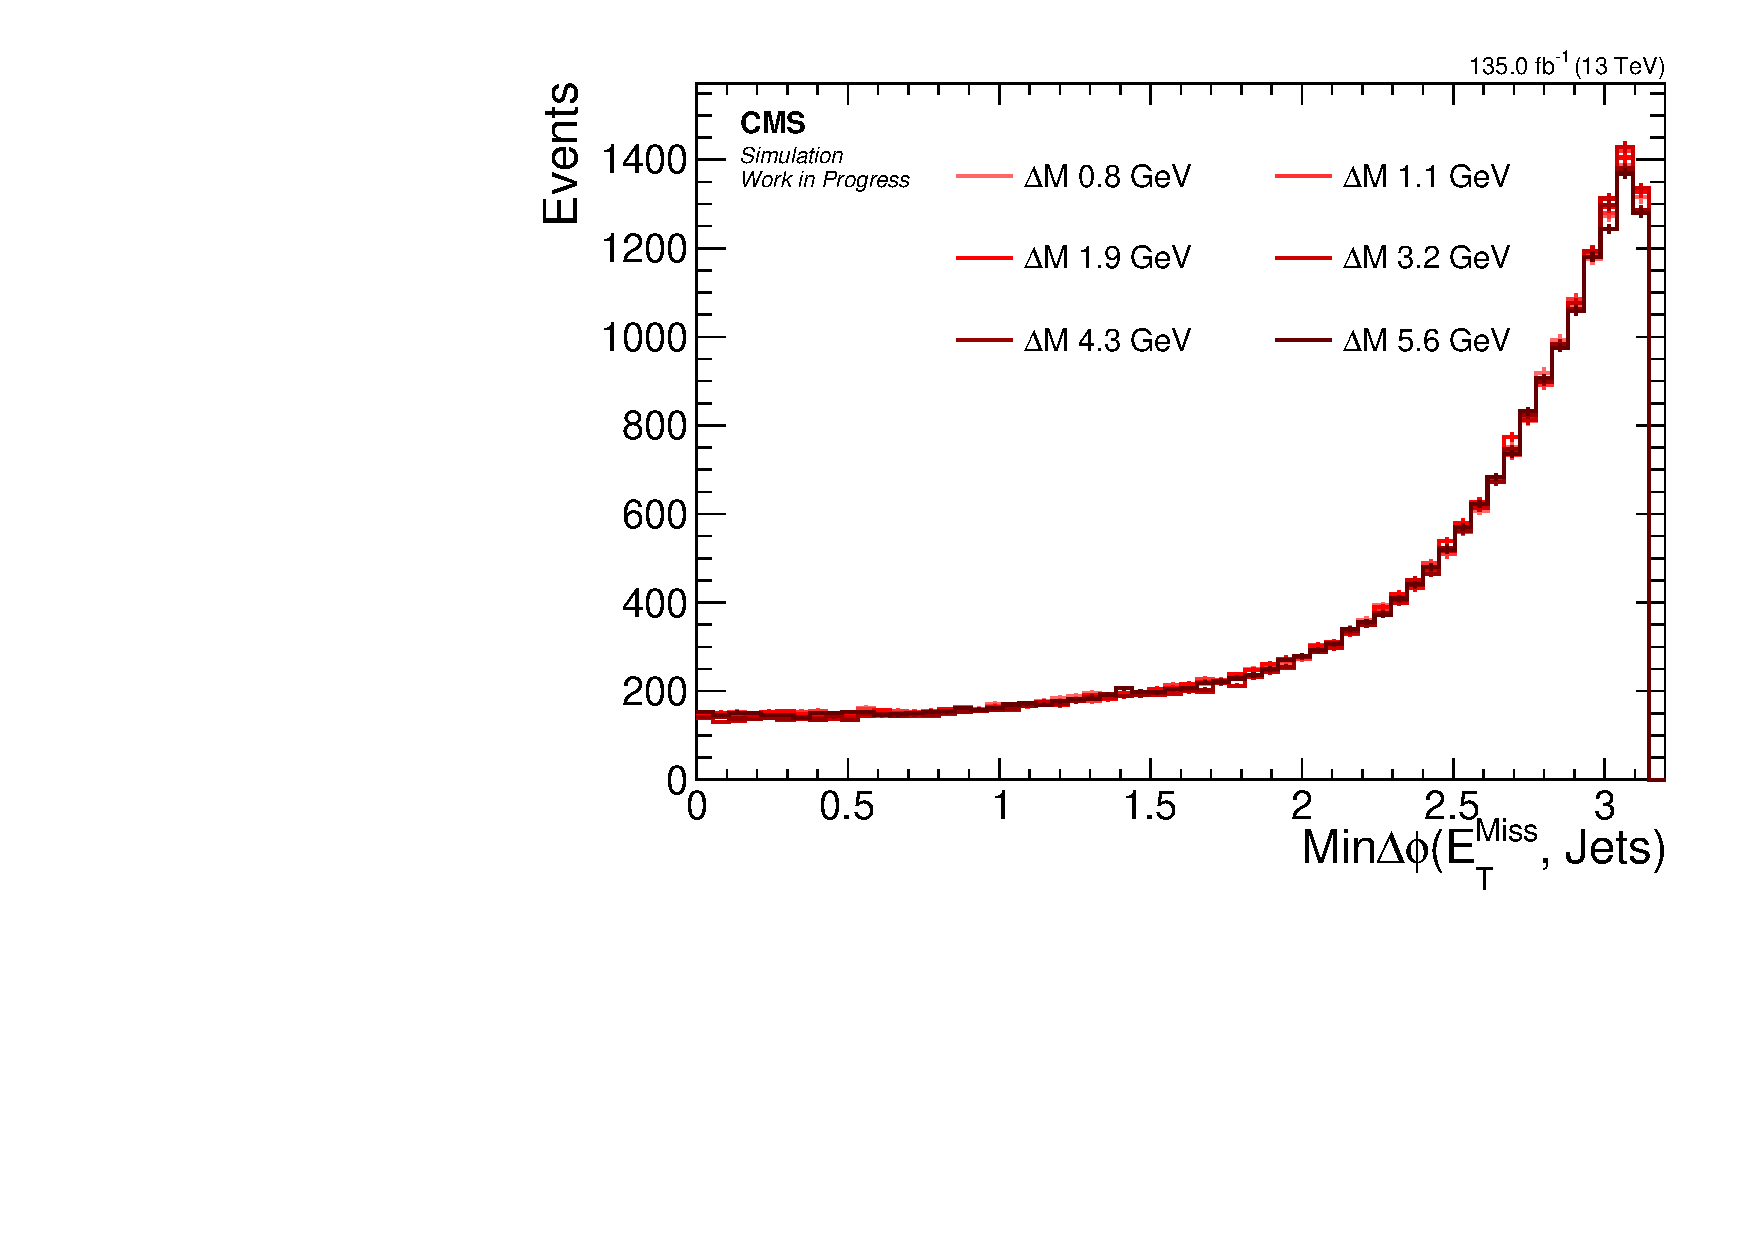
\includegraphics[width=0.48\linewidth]{plots/signal_common_distributions_fixed_mu/none_MinDeltaPhiMetJets.pdf} \,
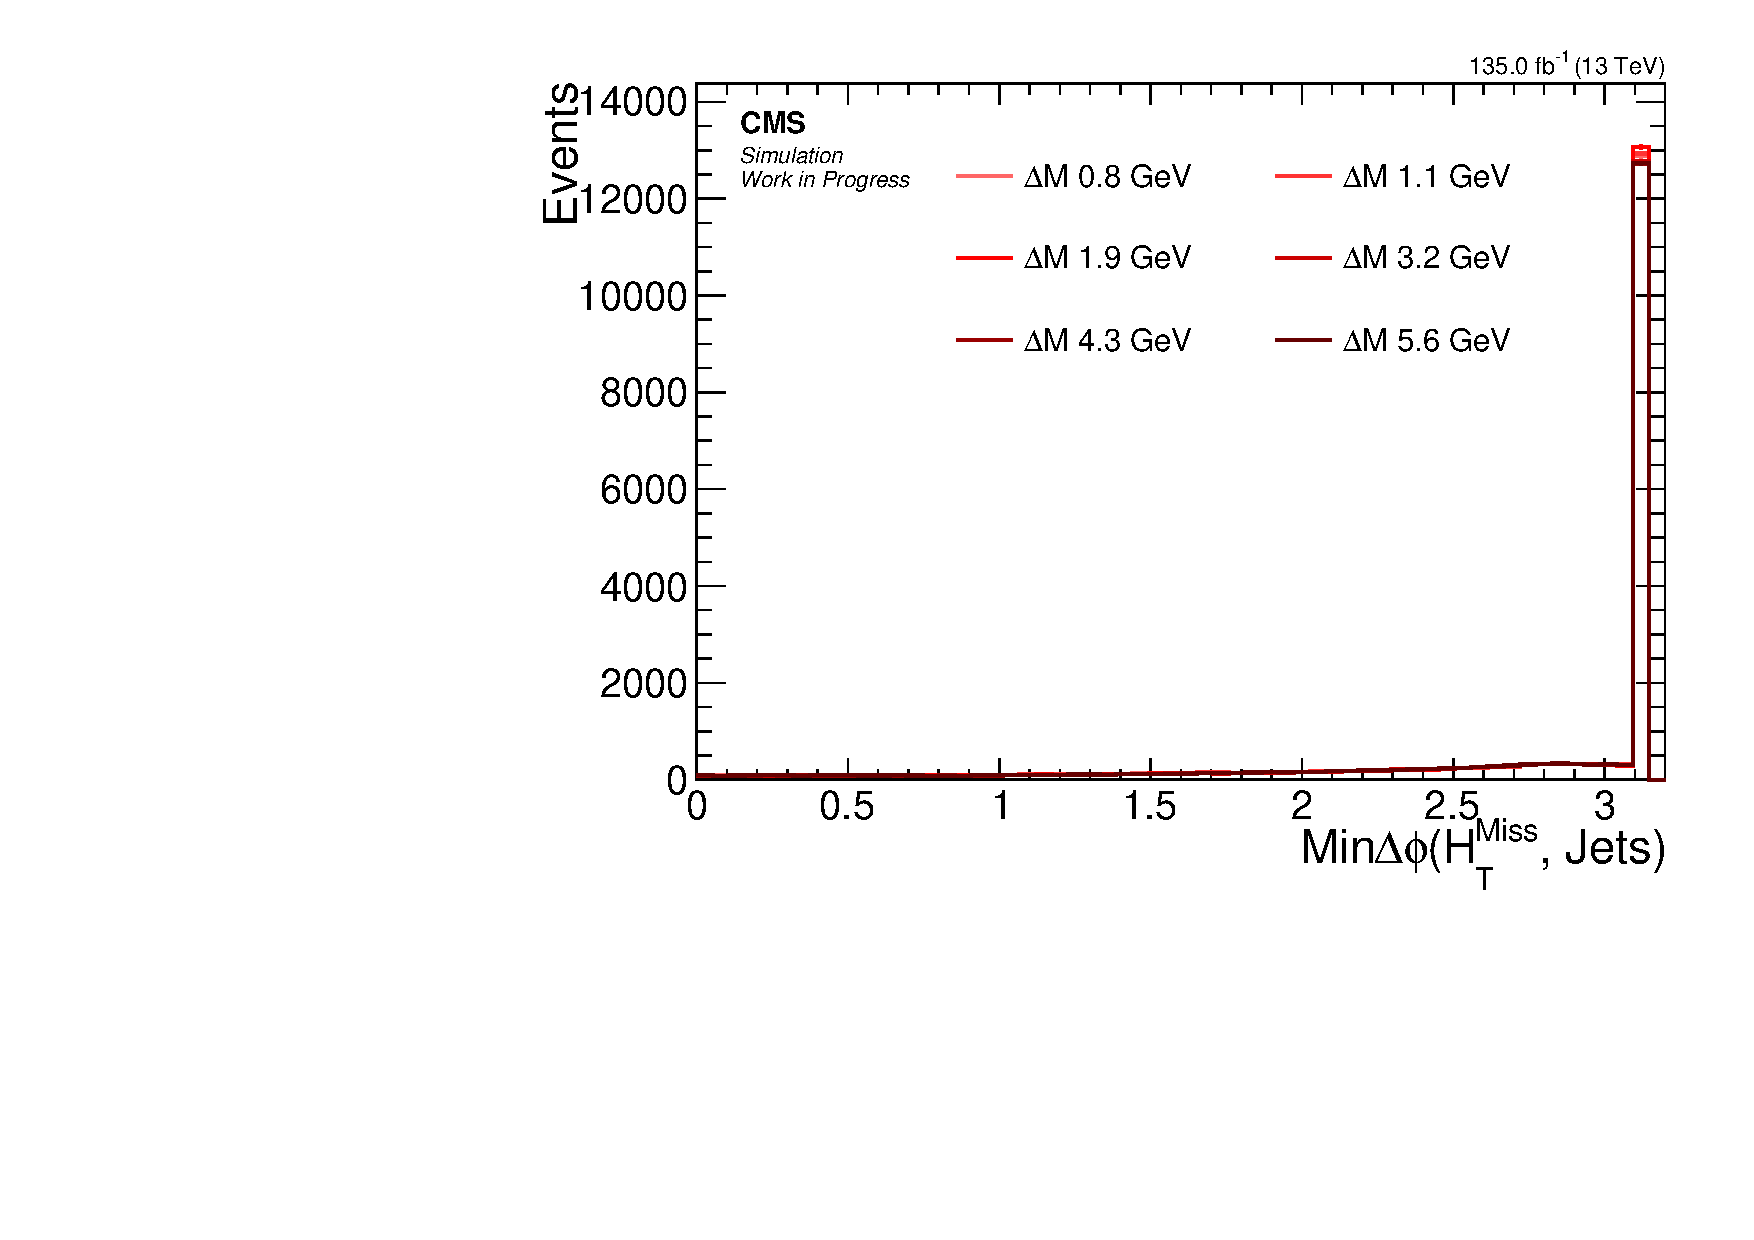
\includegraphics[width=0.48\linewidth]{plots/signal_common_distributions_fixed_mu/none_MinDeltaPhiMhtJets.pdf}  \\
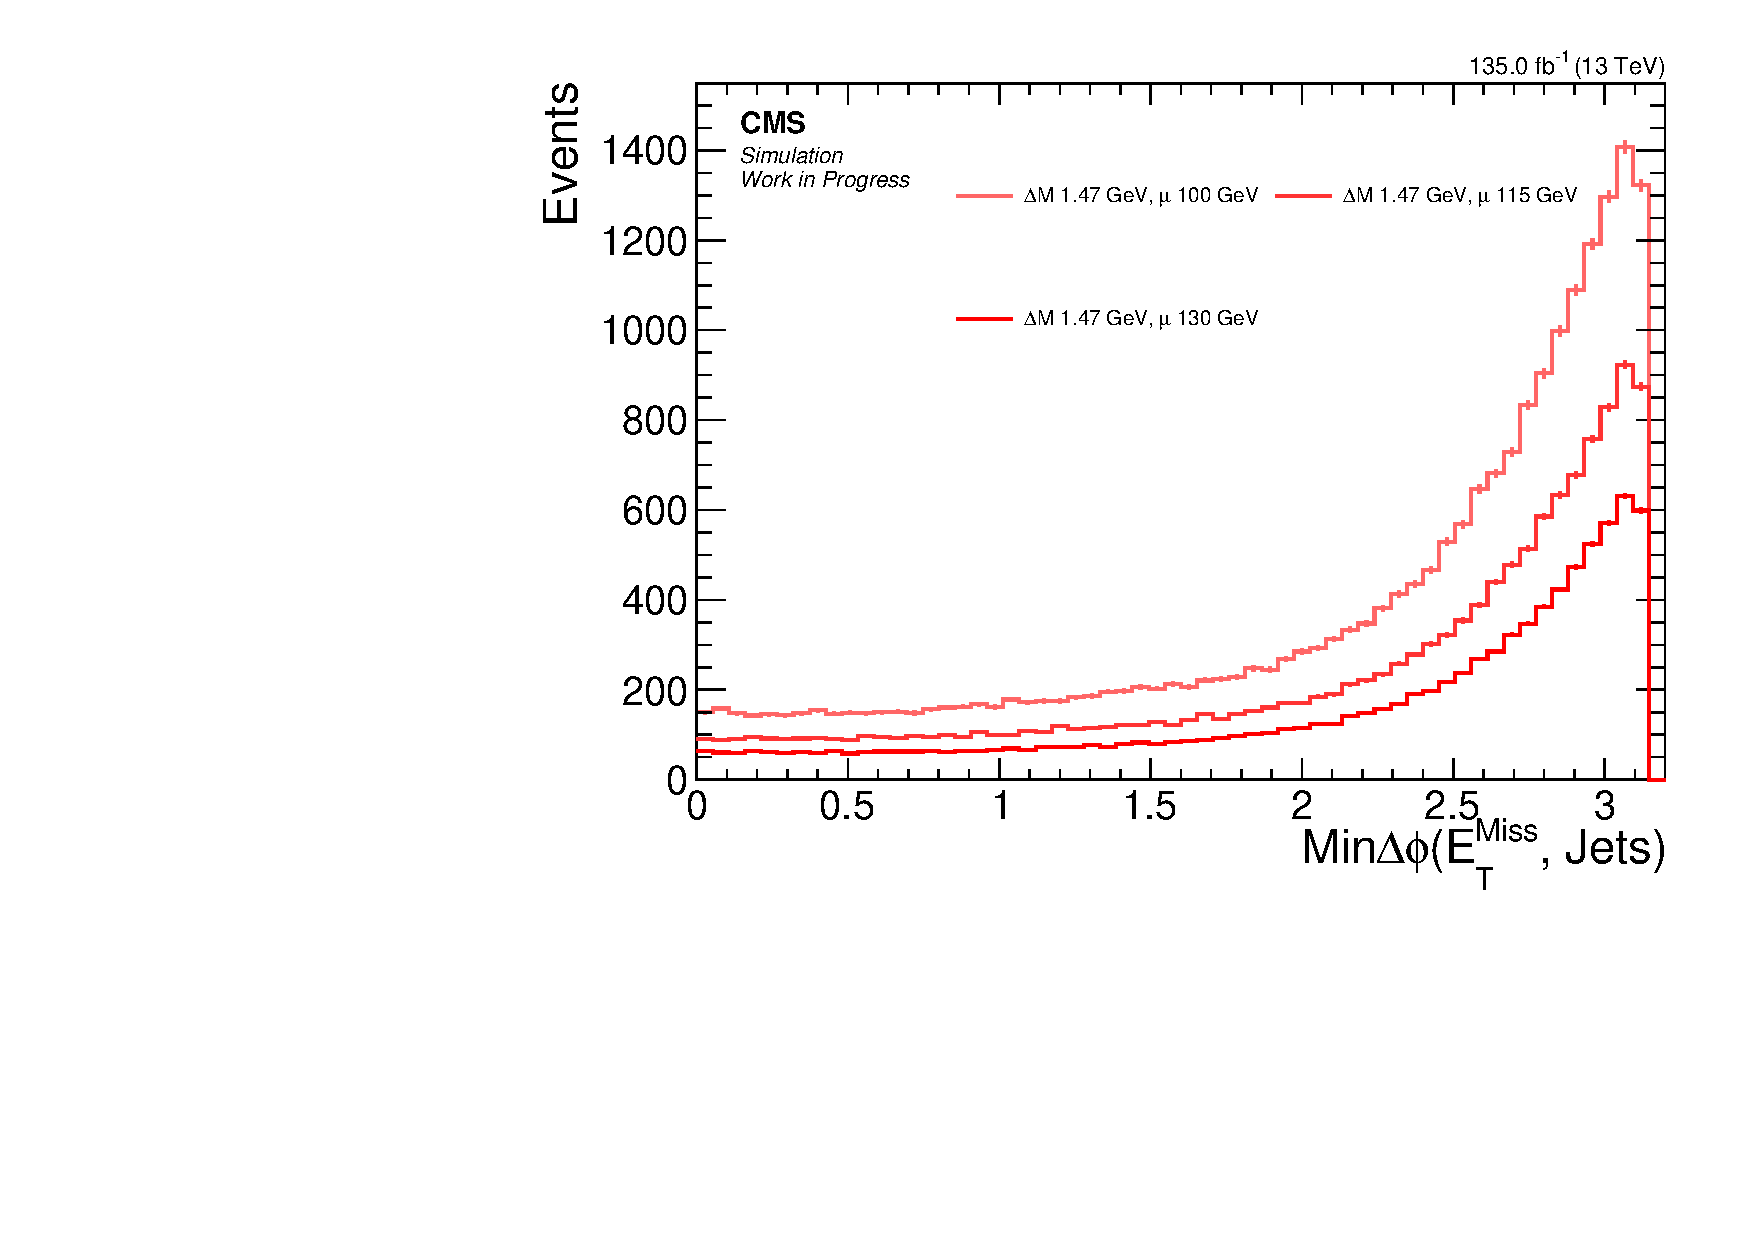
\includegraphics[width=0.48\linewidth]{plots/signal_common_distributions_fixed_dm/none_MinDeltaPhiMetJets.pdf} \,
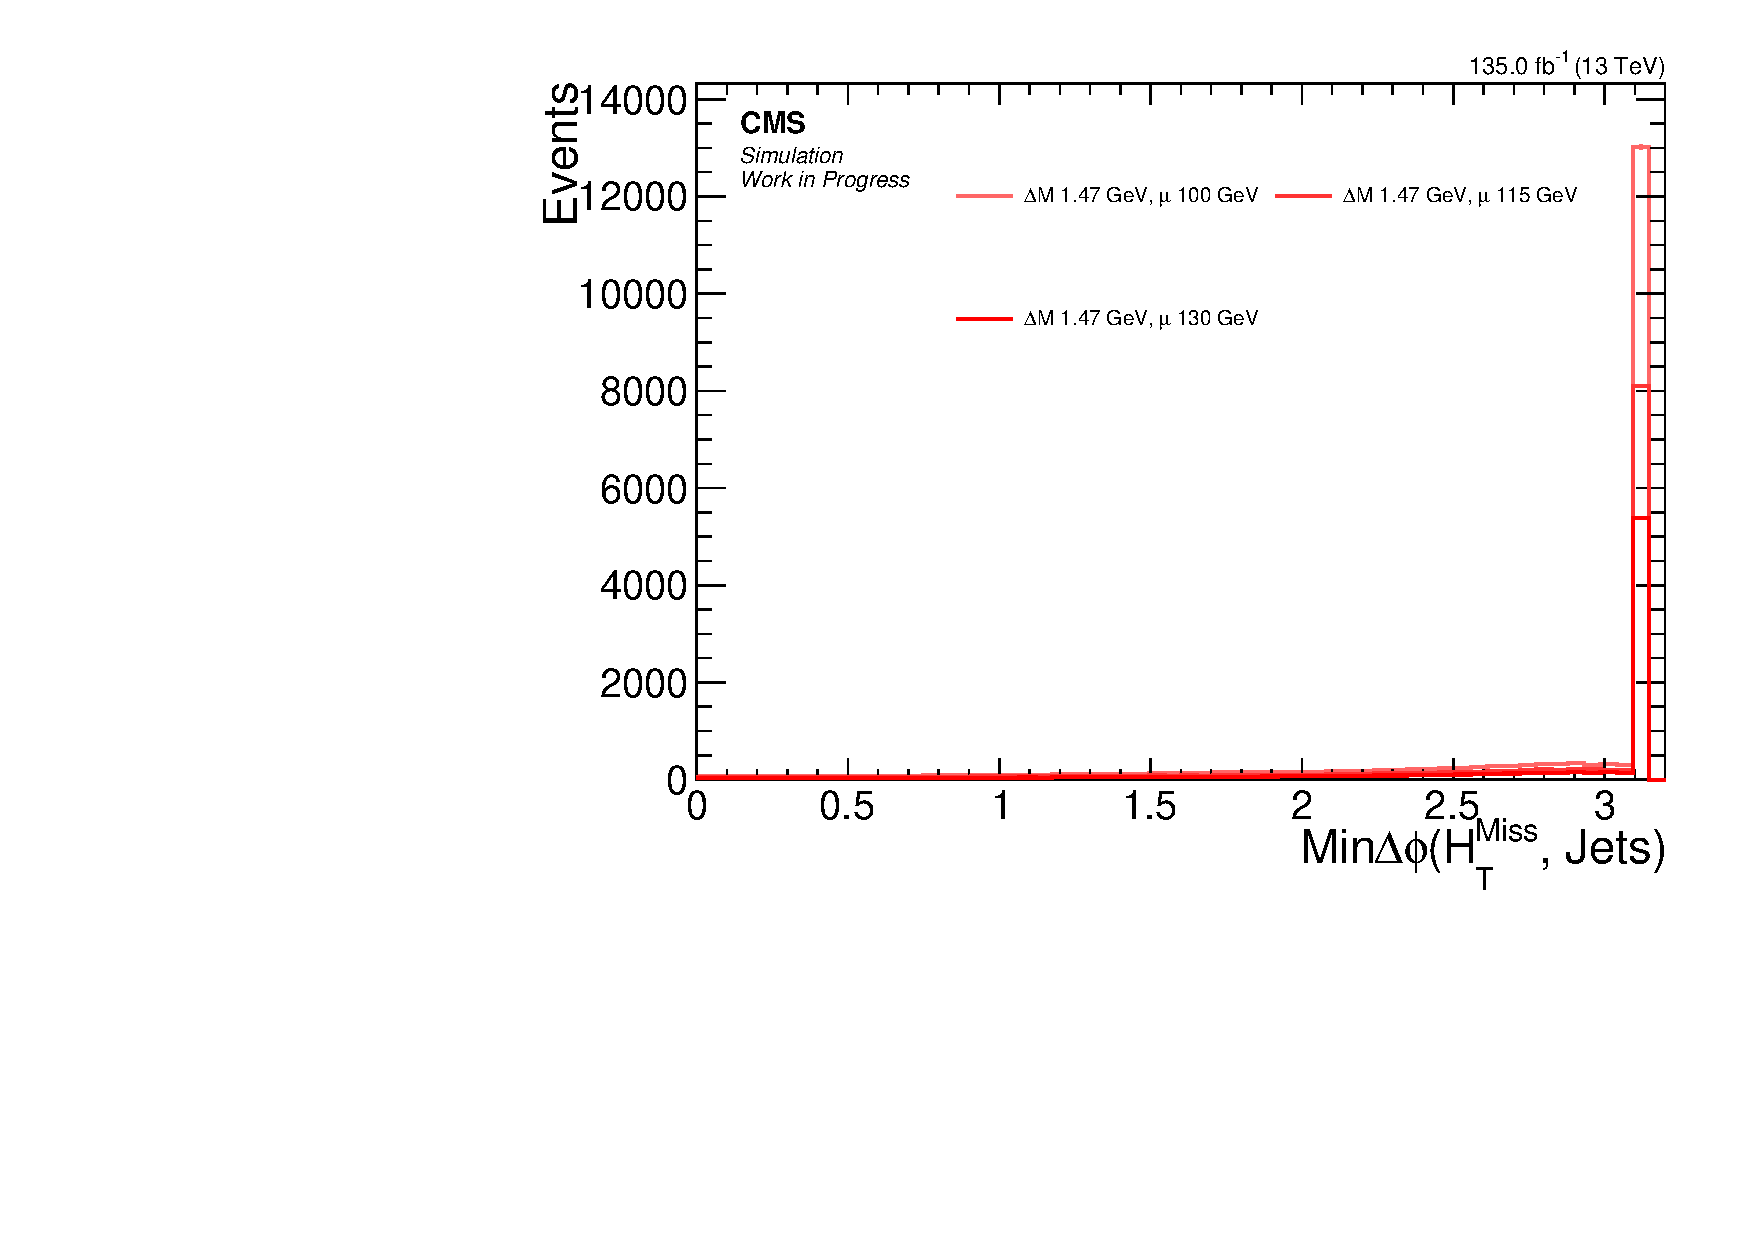
\includegraphics[width=0.48\linewidth]{plots/signal_common_distributions_fixed_dm/none_MinDeltaPhiMhtJets.pdf}  \\
\caption[Signal $\mindphimetjets$ and $\mindphimhtjets$ distributions]{ Signal distributions of \mindphimetjets (left) and \mindphimhtjets (right) comparing various $\dm$ with a fixed higgsino parameter $\mu=100\GeV$ (upper), and comparing various $\mu$ with fixed $\dm=1.47\GeV$ (lower).}
\label{fig:signal-min-deltaphi-met-mht}
\end{figure}

\subsection{Base selection}

The section is recapped by summarizing the base selection of the analysis. The base selection, also known interchangeably as the preselection, is applied to all analysis categories. It ls listed in Table~\ref{tab:base-selection}.

\begin{table}[!htb]
	\centering
	\label{tab:base-selection}
		\caption{The preselection criteria, which are applied to all analysis categories.}
		%\vspace{1mm}
			\begin{tabular}{lc} \hline
			Variable & Value \\ \hline
			$\mht \left[\GeV\right]$ & $>220$ \\
			$\njets \left( \pt \geq 30\GeV\, \mathrm{and}\, \abs{\eta} < 2.4 \right)$ & $\geq 1$\\
			$\nbjets \left( \pt \geq 30\GeV\, \mathrm{and}\, \abs{\eta} < 2.4 \right)$ & =0 \\
			$\mindphimhtjets$ & $ > 0.4$ \\ \hline
			\end{tabular}
\end{table}

\clearpage
\subsection{Lepton kinematics}

The hadronic component of signal events has been the focus up until this point. However, the dilepton system contains the most distinctive features of the signal. To fully understand the unique phase space of the dilepton system, generator level distributions are examined first, followed by an exploration of the effects of reconstruction on those observables. Since the dimuon category is the most sensitive and because the logic applies analogously to the two-electron final state, the electron category is excluded from the following sections. The lepton kinematics change dramatically as a function of \dm. In contrast, the higgsino parameter $\mu$ effects almost only the overall normalization due to the different production cross section. Therefore, the higgsino parameter is set to $\mu=100\GeV$ in the following sections, with the \dm varied.

\subsubsection{Lepton $\eta$ and transverse momentum \gls{pt}}
\label{sec:muon-eta-pt}

The signal acceptance and sensitivity are significantly impacted by the thresholds of the transverse momentum \gls{pt} distribution of the muons that make it through the reconstruction and identification. The selection applied to the muons in this analysis is described in Section~\ref{sec:muon-selection} and referred to as the \emph{analysis selection}. This section aims to examine the importance of the \gls{pt} on the signal and its dilepton kinematic distributions.

The generator level distribution of \gls{pt}, or the so-called \emph{truth} distributions, which do not exhibit any detector or reconstruction features, are examined first. The distribution of reconstructed \pt is then compared with the generator level distribution in Figure~\ref{fig:signal-muons-pt}. 

\begin{figure}[!htb]
\centering
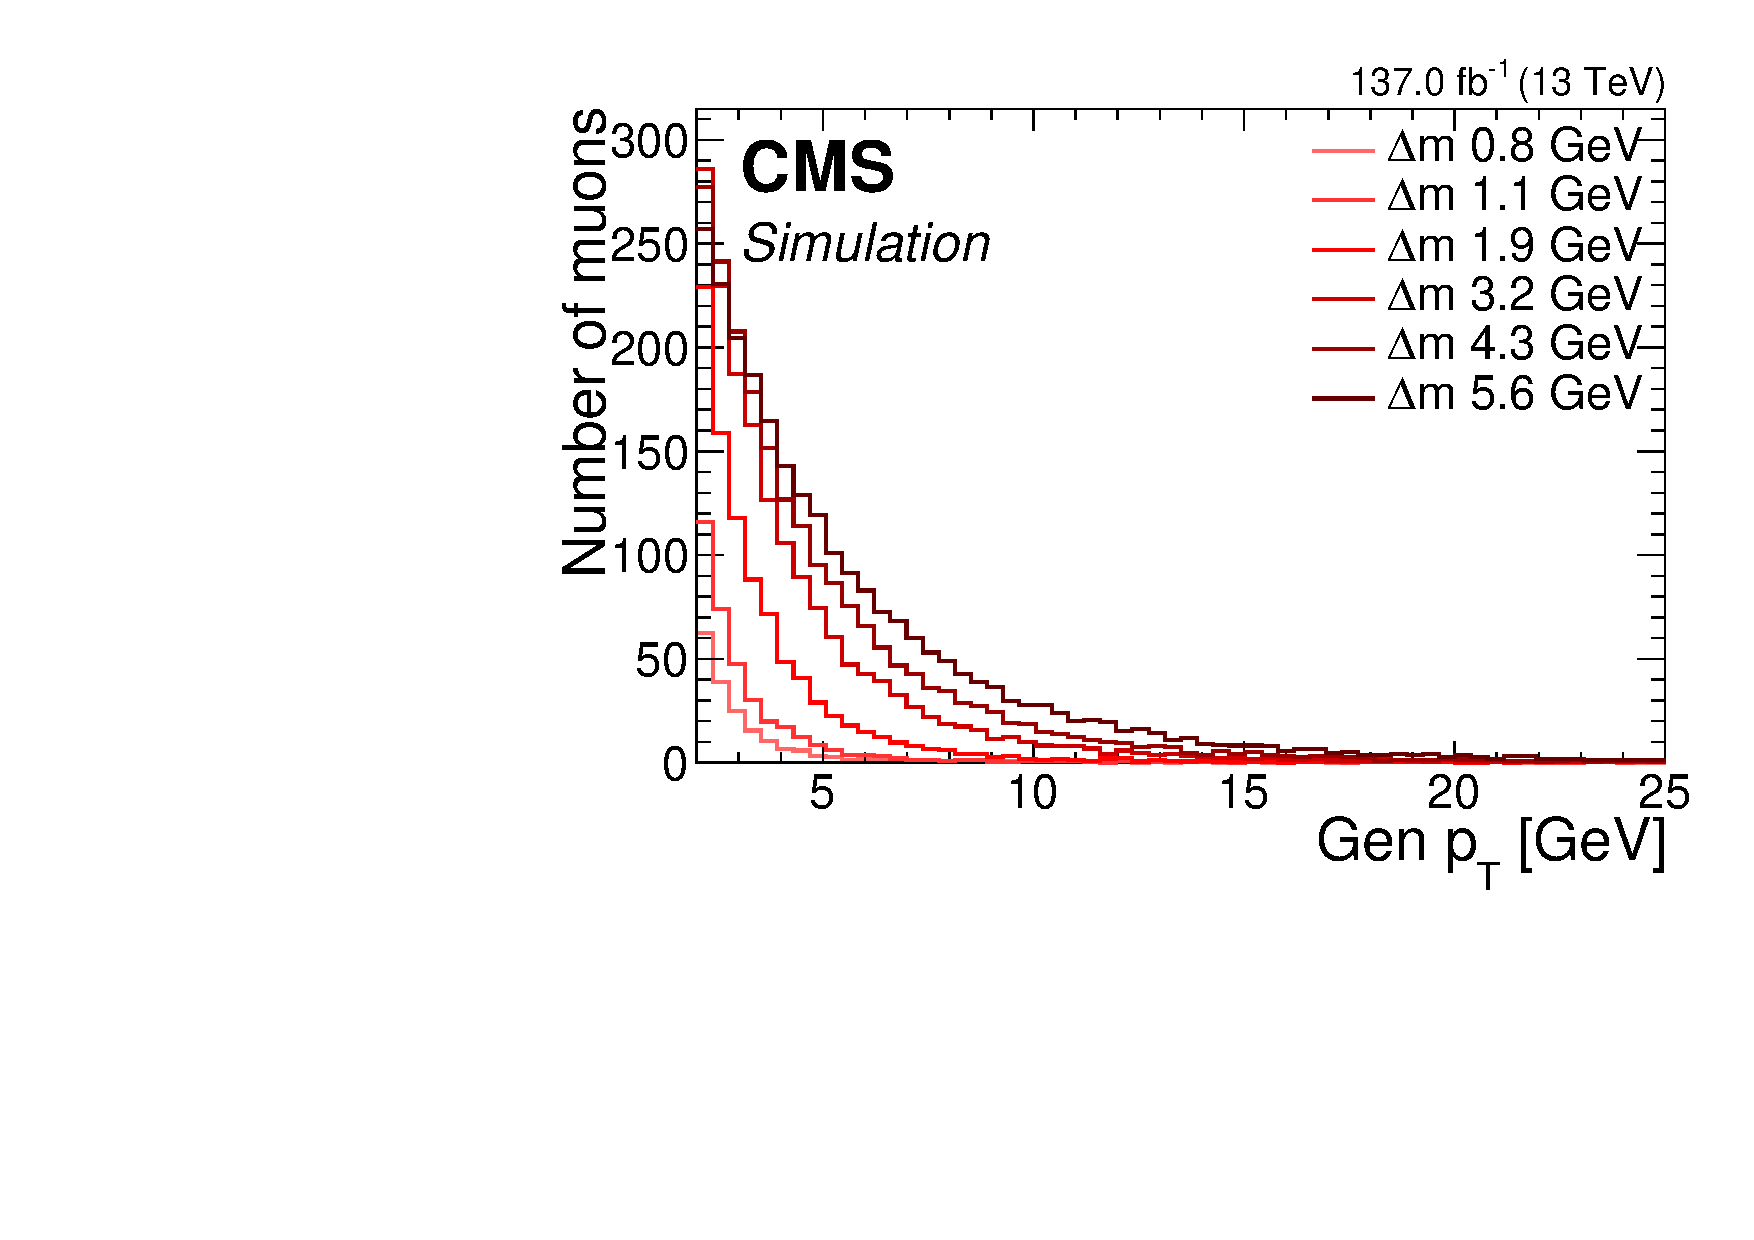
\includegraphics[width=0.32\linewidth]{plots/signal_muons_gen/none_Muons_pt.pdf} \,
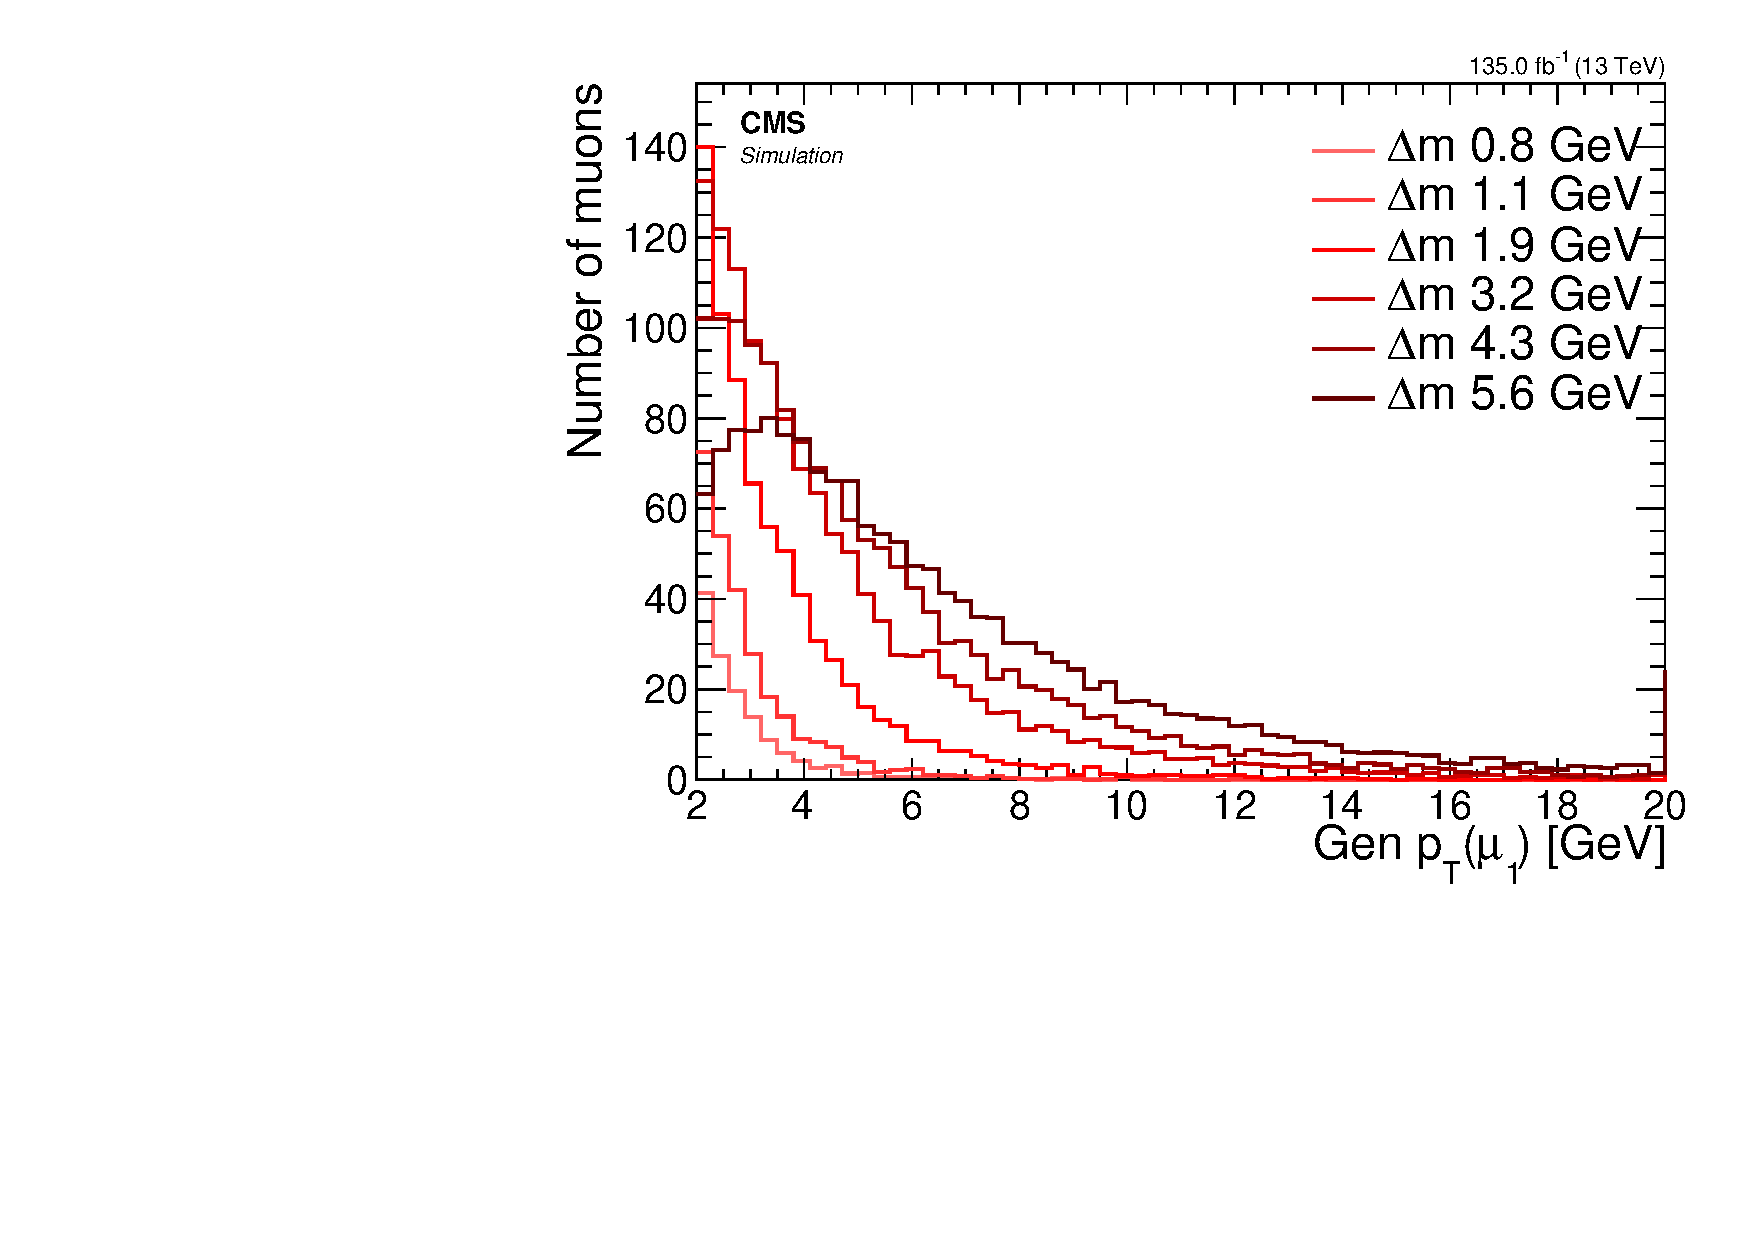
\includegraphics[width=0.32\linewidth]{plots/signal_muons_gen/none_Muons_m1_pt.pdf}  \,
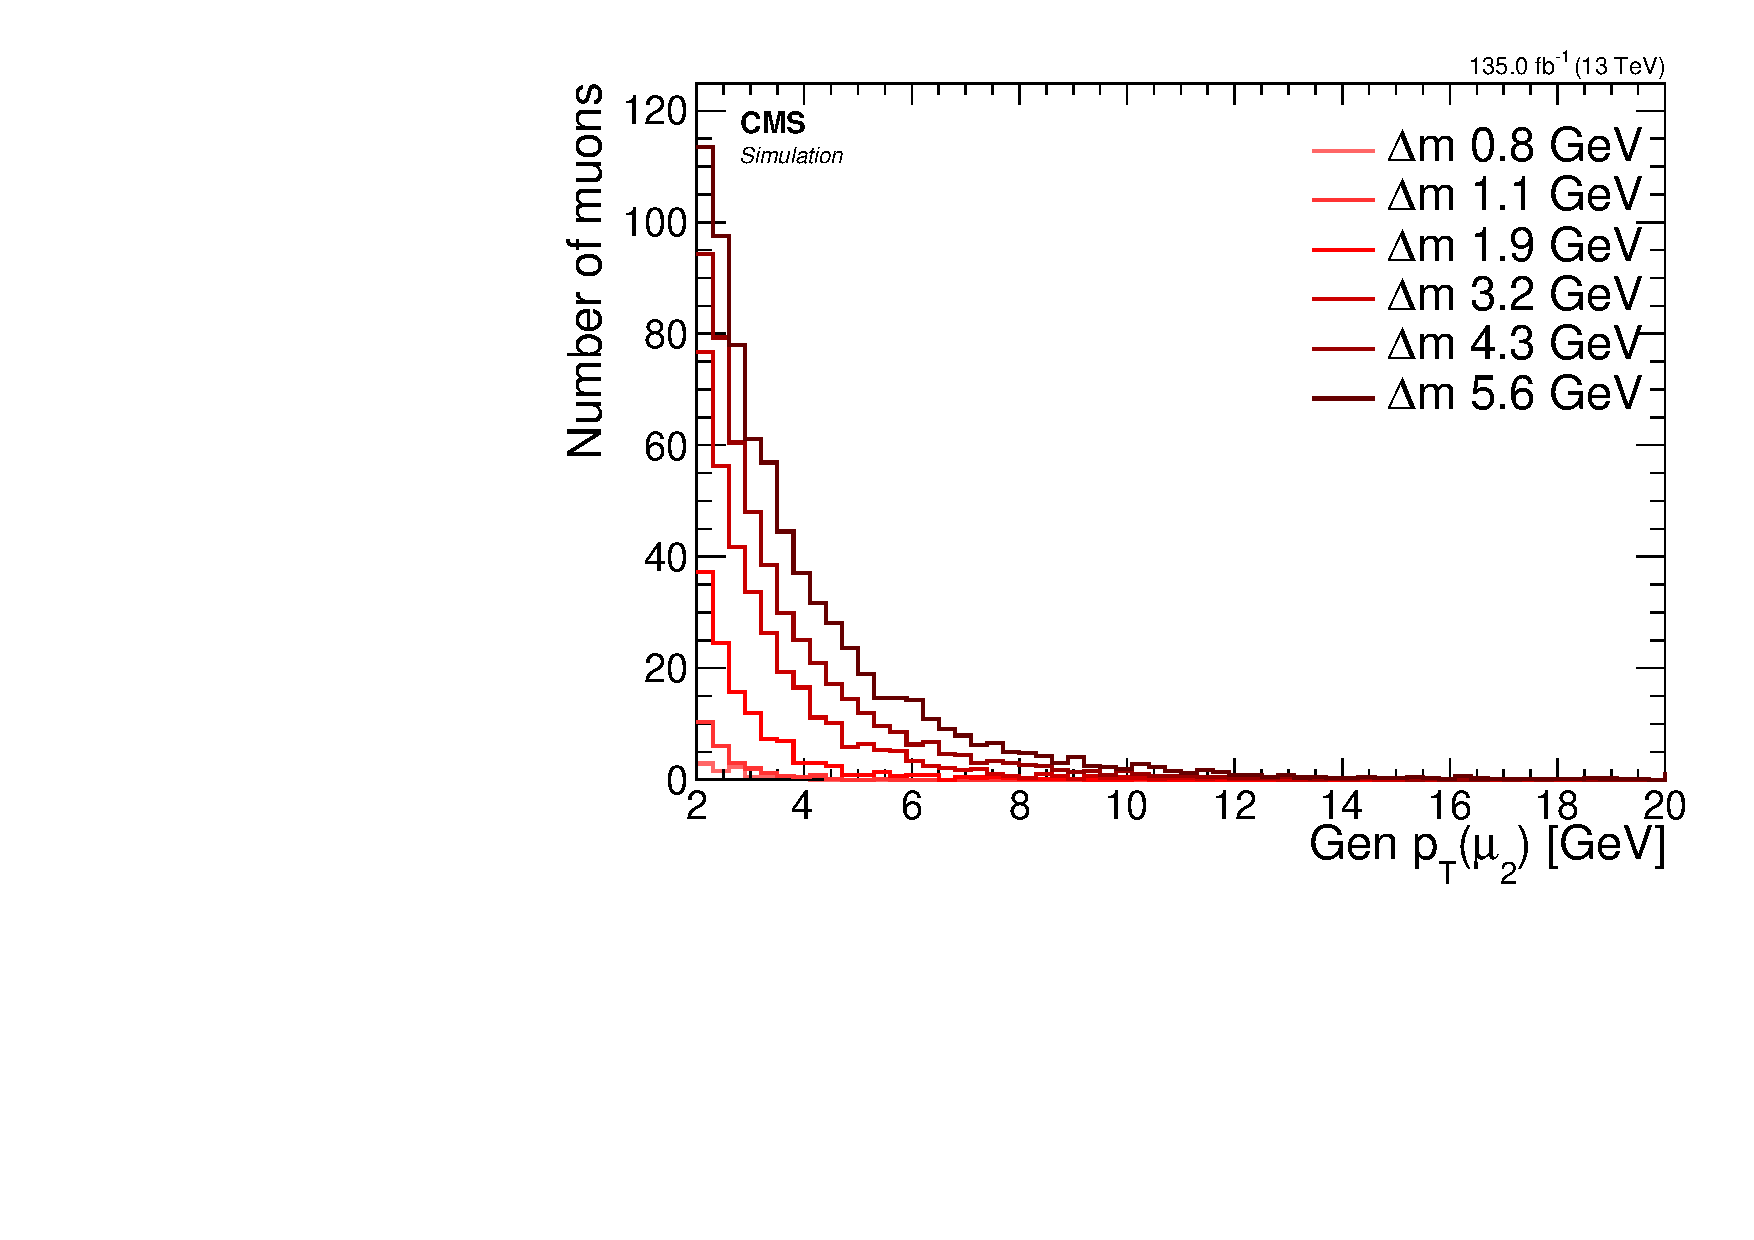
\includegraphics[width=0.32\linewidth]{plots/signal_muons_gen/none_Muons_m2_pt.pdf} \\
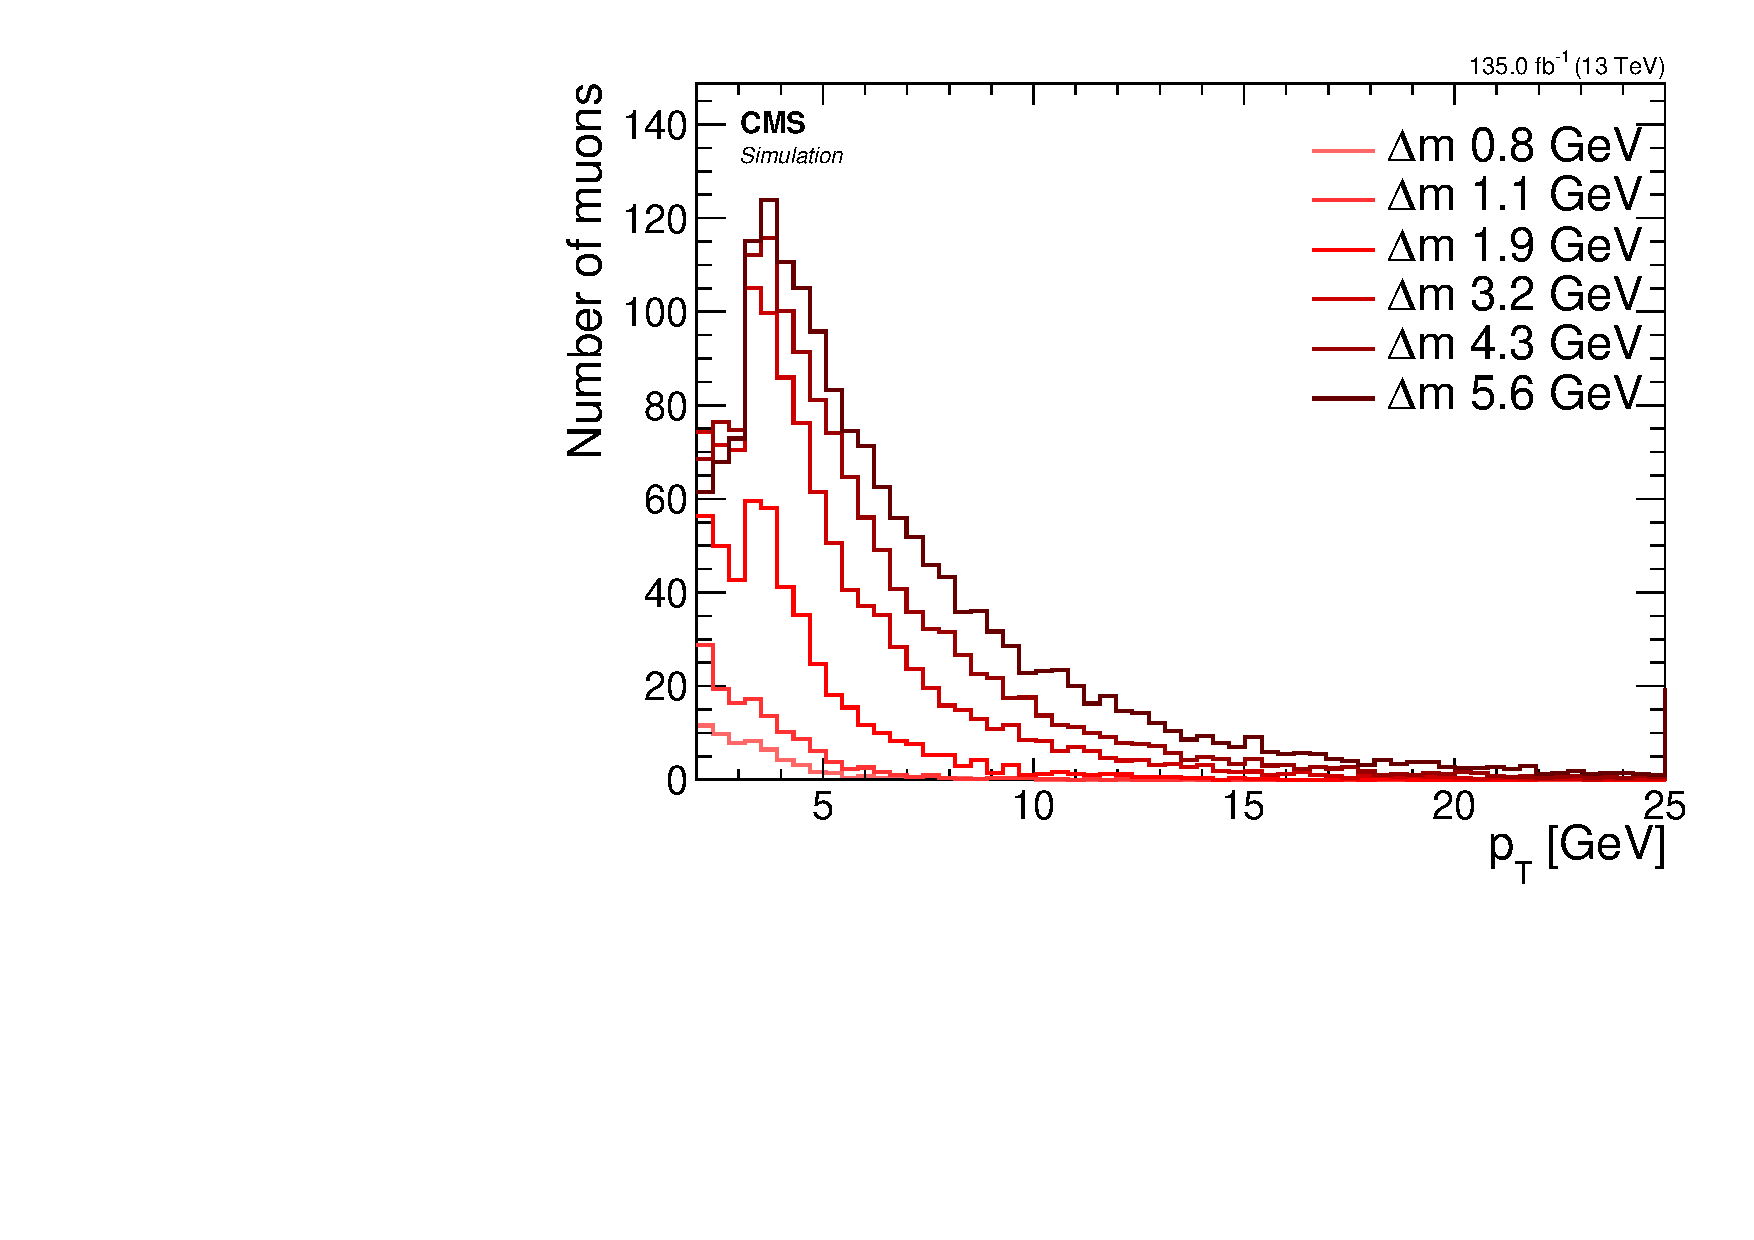
\includegraphics[width=0.32\linewidth]{plots/signal_muons/none_Muons_pt.pdf} \,
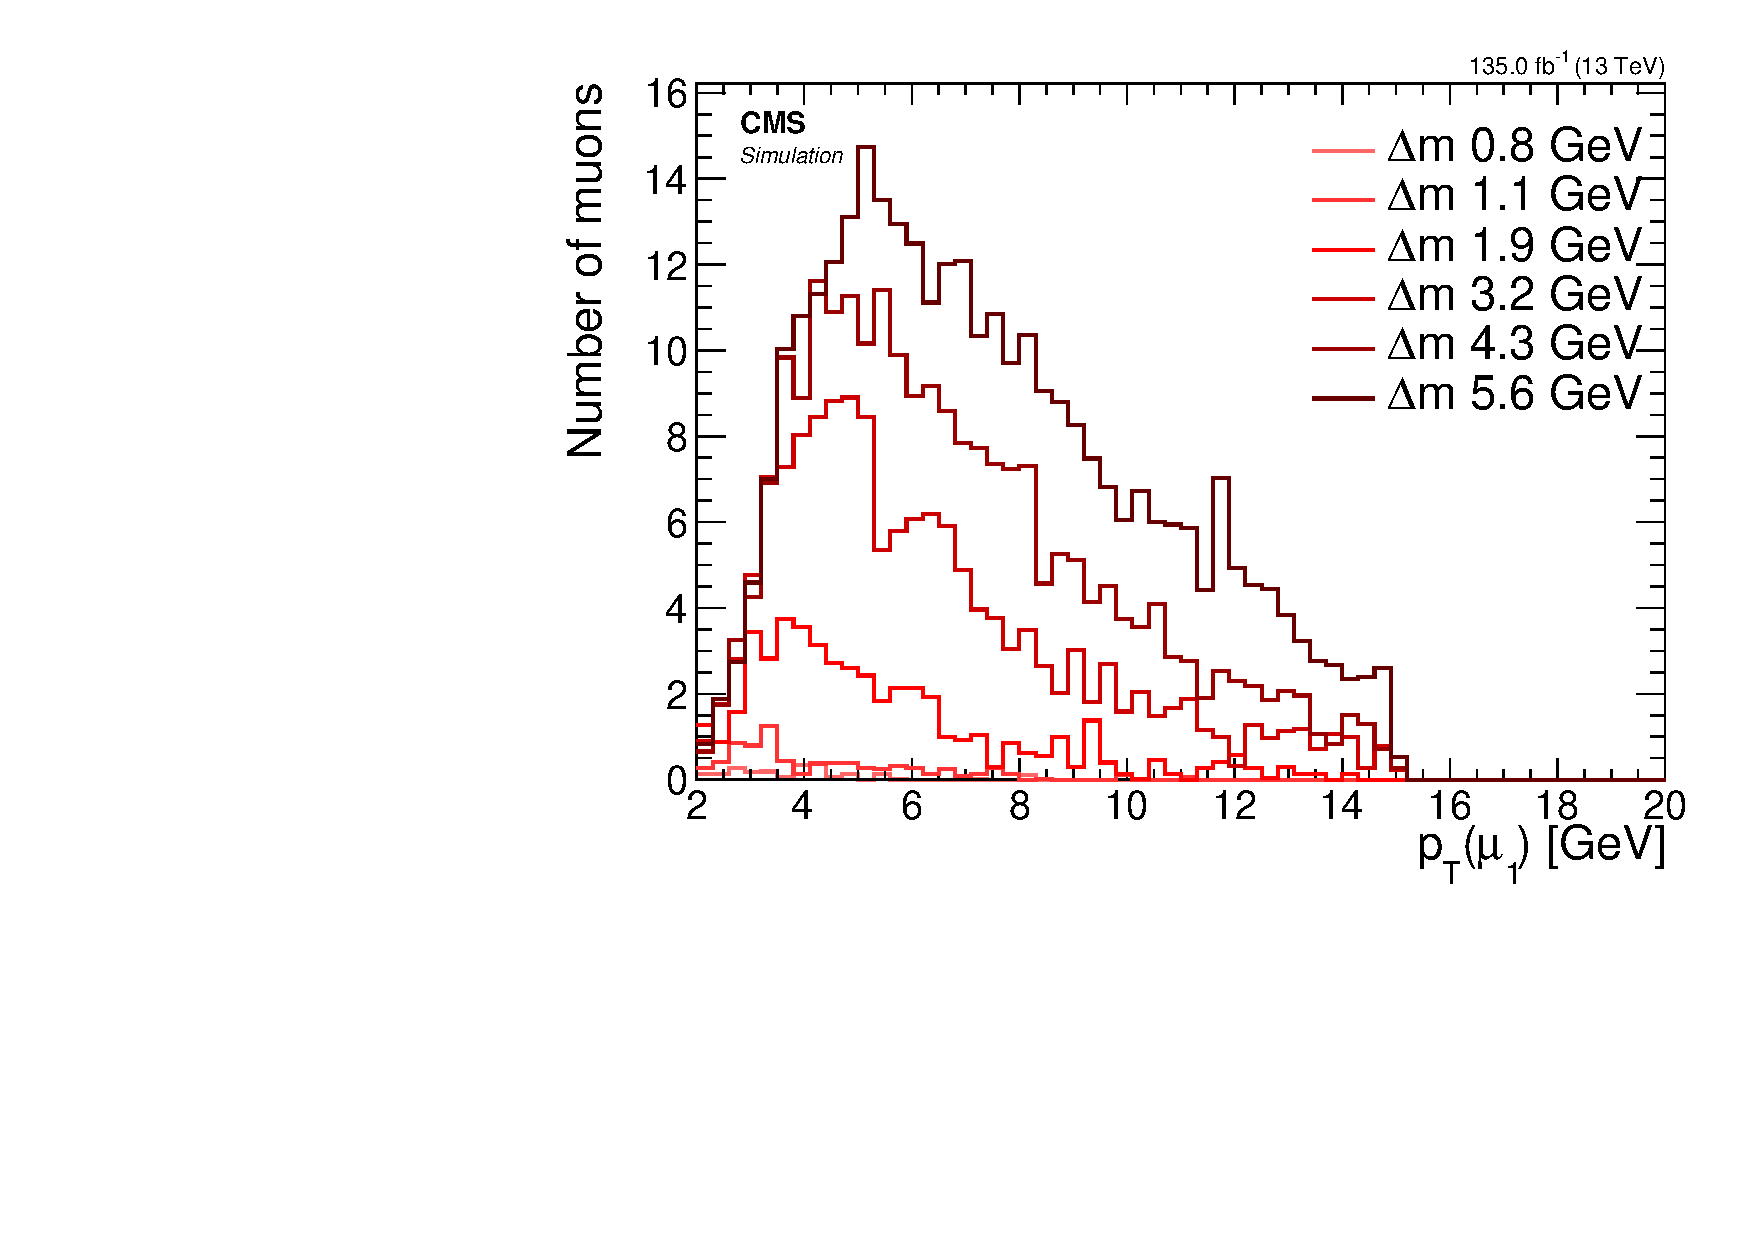
\includegraphics[width=0.32\linewidth]{plots/signal_muons/none_Muons_m1_pt.pdf}  \,
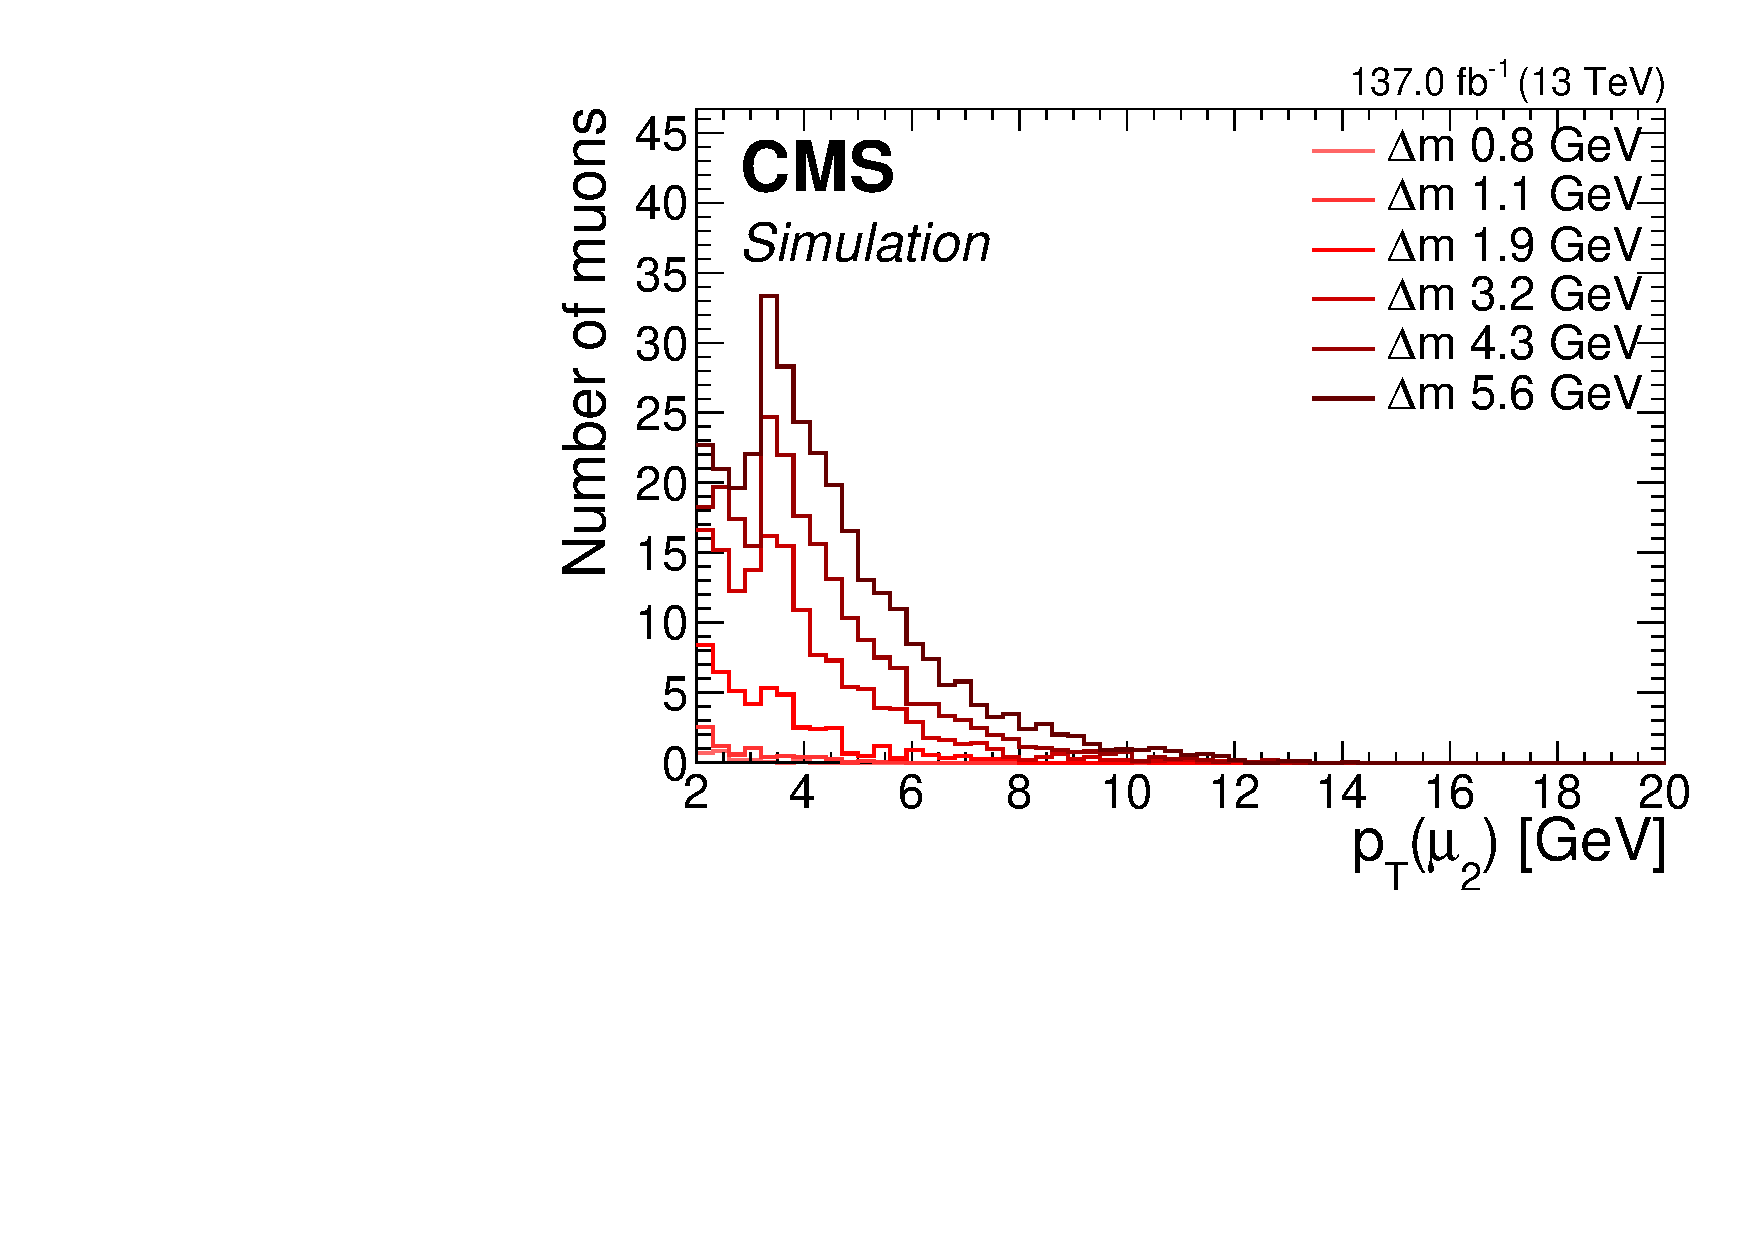
\includegraphics[width=0.32\linewidth]{plots/signal_muons/none_Muons_m2_pt.pdf} \\
\caption[Signal \pt distributions]{ Signal \pt distributions for inclusive (left), leading muon $\mu_1$ (middle),  subleading muon $\mu_2$ (right) at generator level (top) and reconstruction level passing analysis selection (bottom). }
\label{fig:signal-muons-pt}
\end{figure}

When comparing the generator level and reconstruction level inclusive \pt distributions, it becomes apparent that a reshaping occurs around $3 \GeV$. A significant proportion of the generated muons with $\pt<3\GeV$ are lost in the reconstruction process. The subleading muon \pt distribution at the reconstruction level has a camel shape, whereby the efficiency drops below a \pt of $3\GeV$ to about half its maximum value and is only partially regained at $\pt<3\GeV$. This effect is due to the detector geometry and is more clearly visible when splitting the \pt distribution into a barrel ($\abs{\eta} < 1.2$) and encaps ($\abs{\eta} \geq 1.2$) portions, as shown in Figure~\ref{fig:signal-pt-barrel-endcaps}.

\begin{figure}[!htb]
\centering
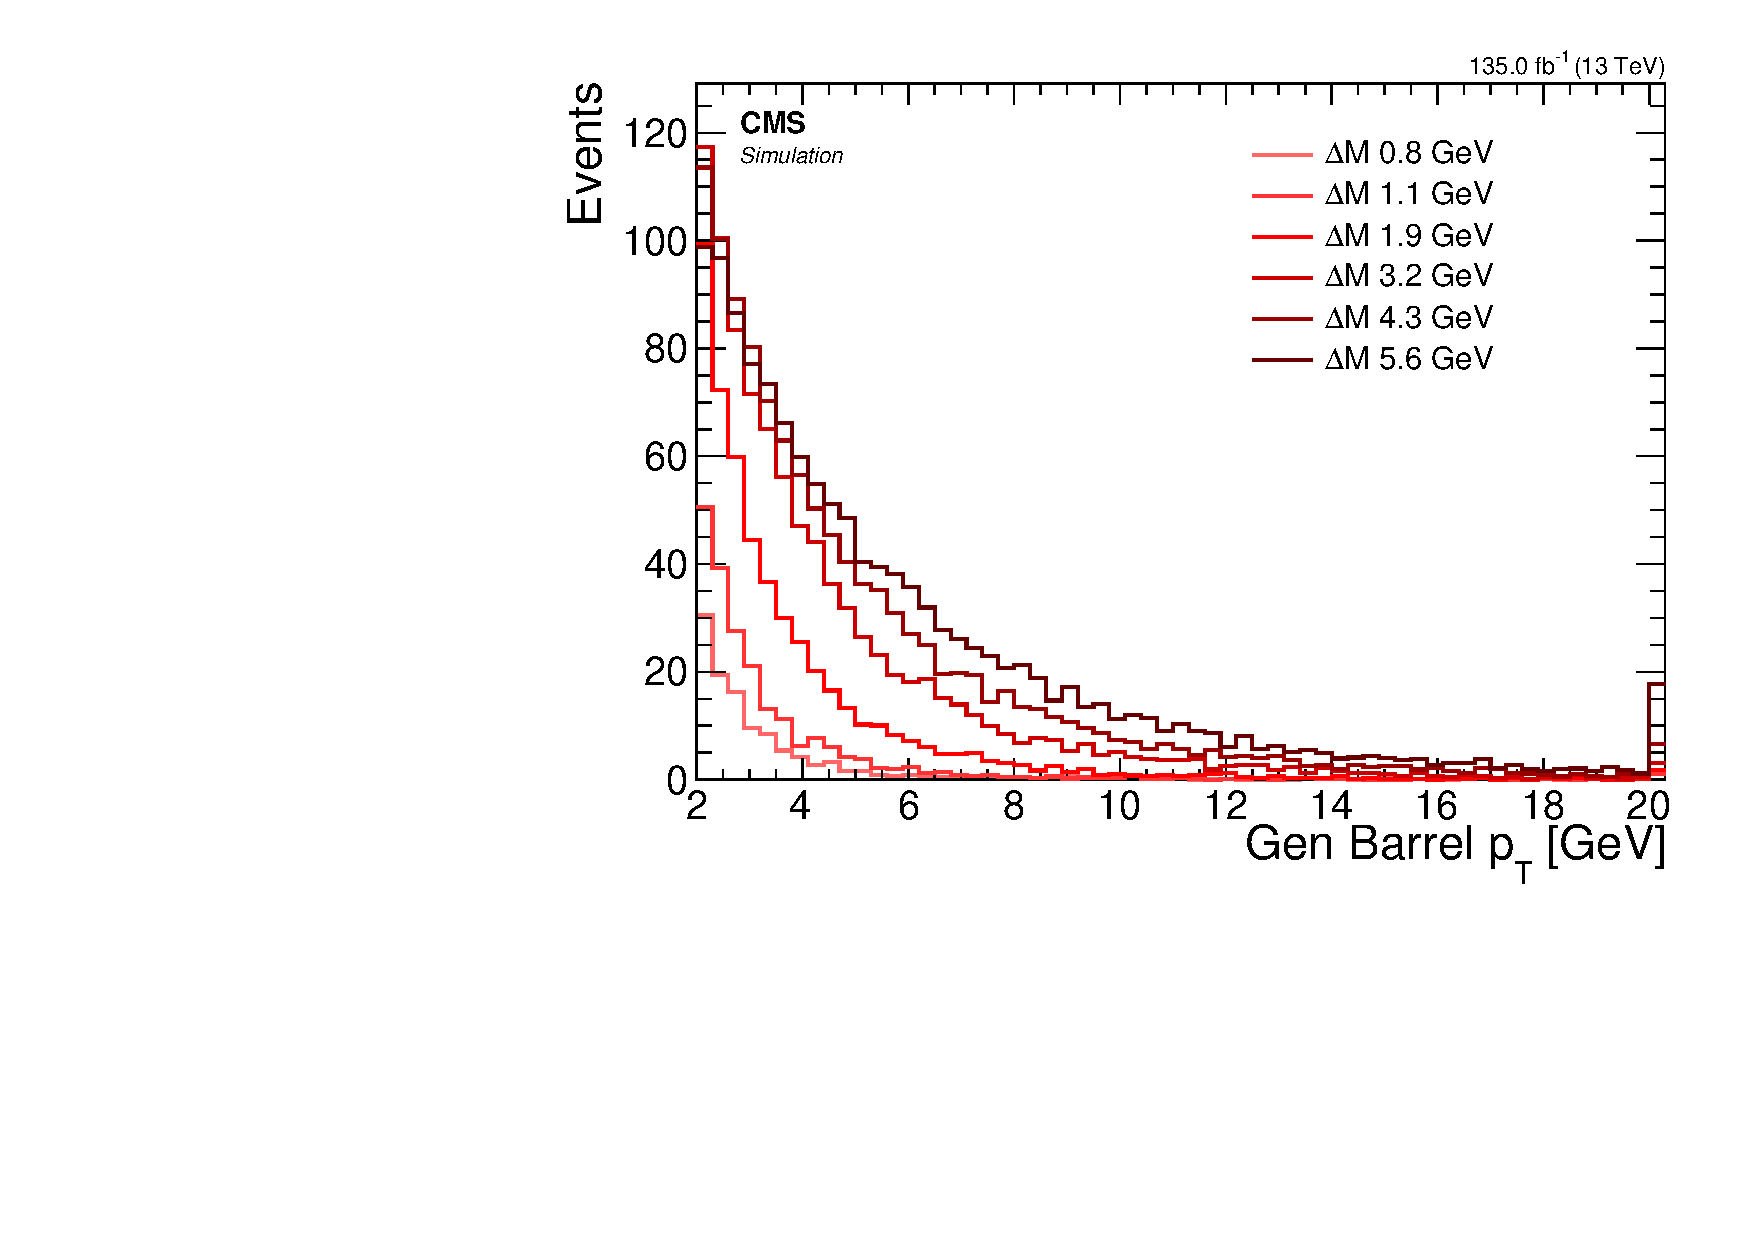
\includegraphics[width=0.48\linewidth]{plots/signal_muons_gen/none_Muons_pt_barrel.pdf} \,
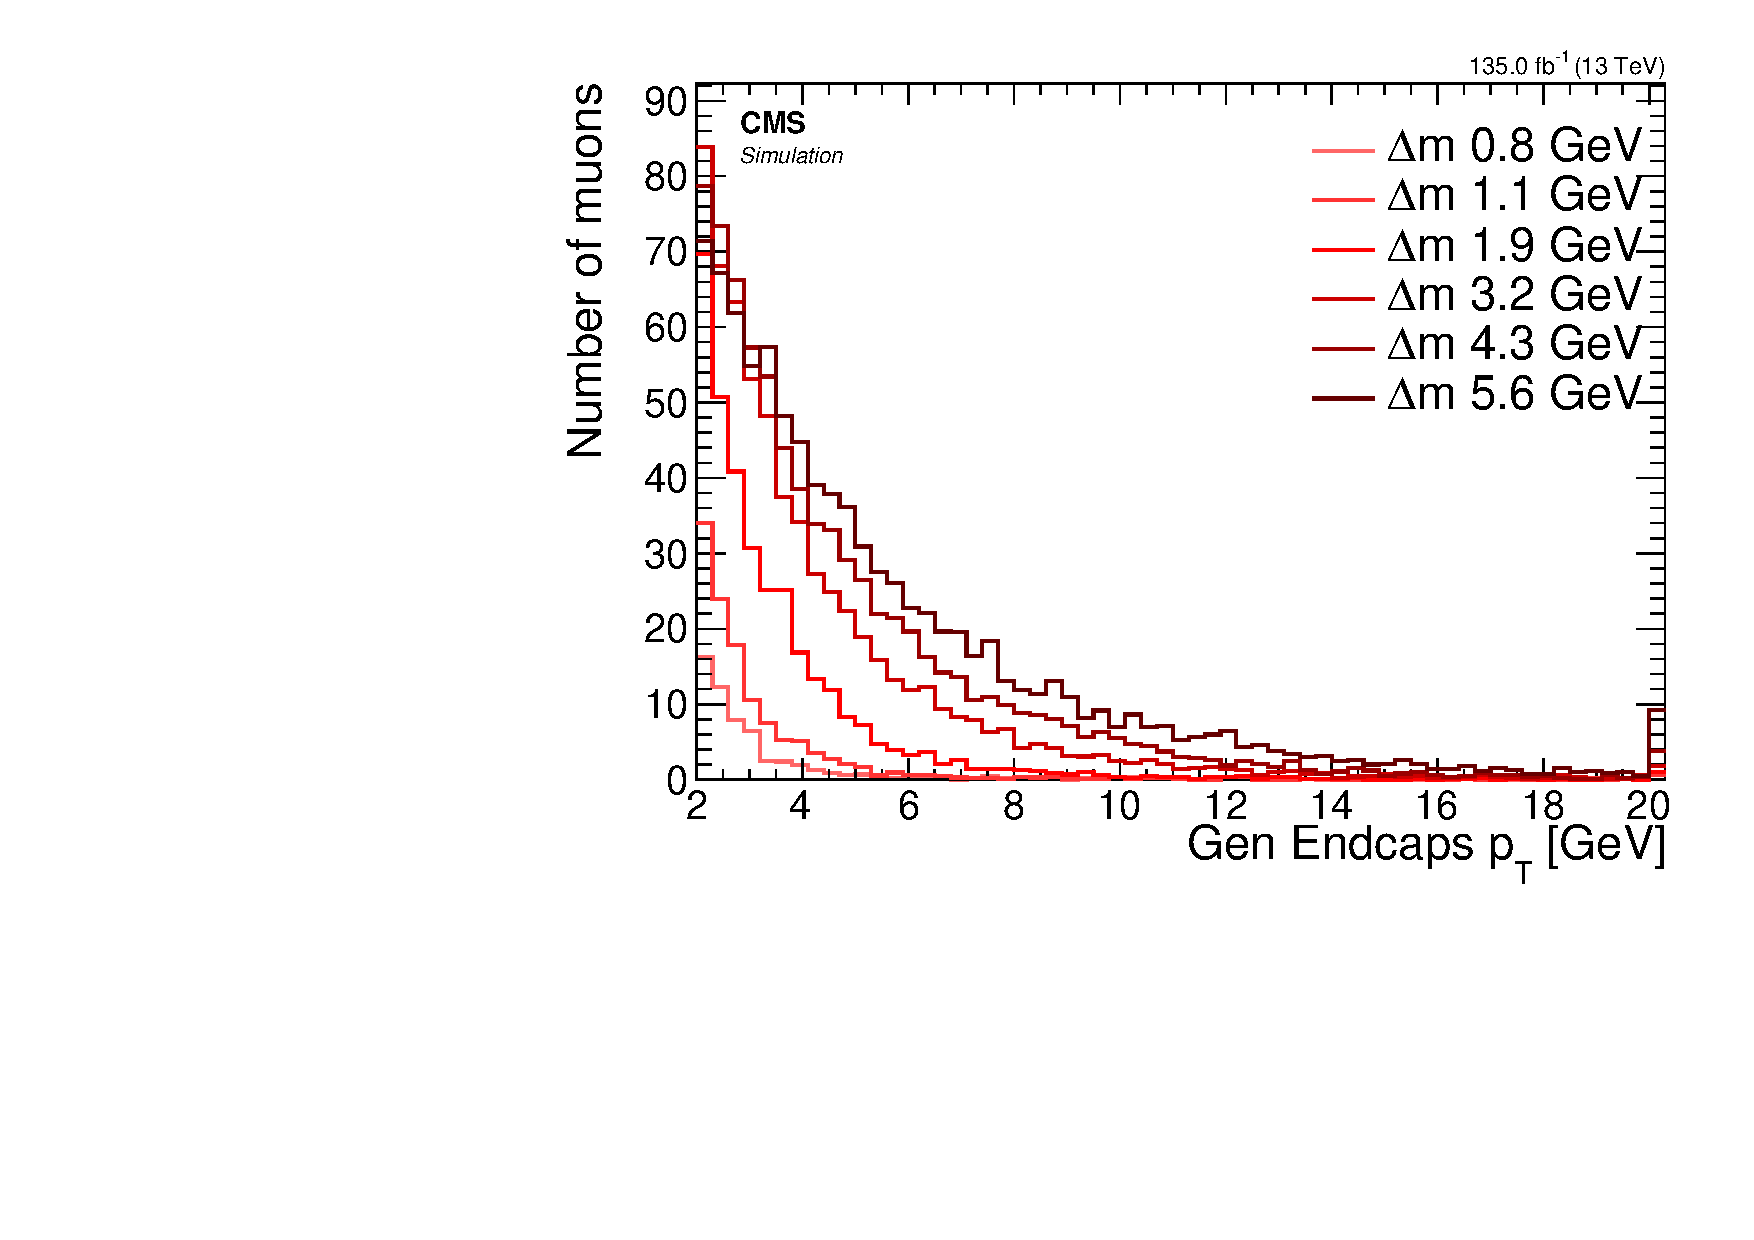
\includegraphics[width=0.48\linewidth]{plots/signal_muons_gen/none_Muons_pt_endcape.pdf}  \\
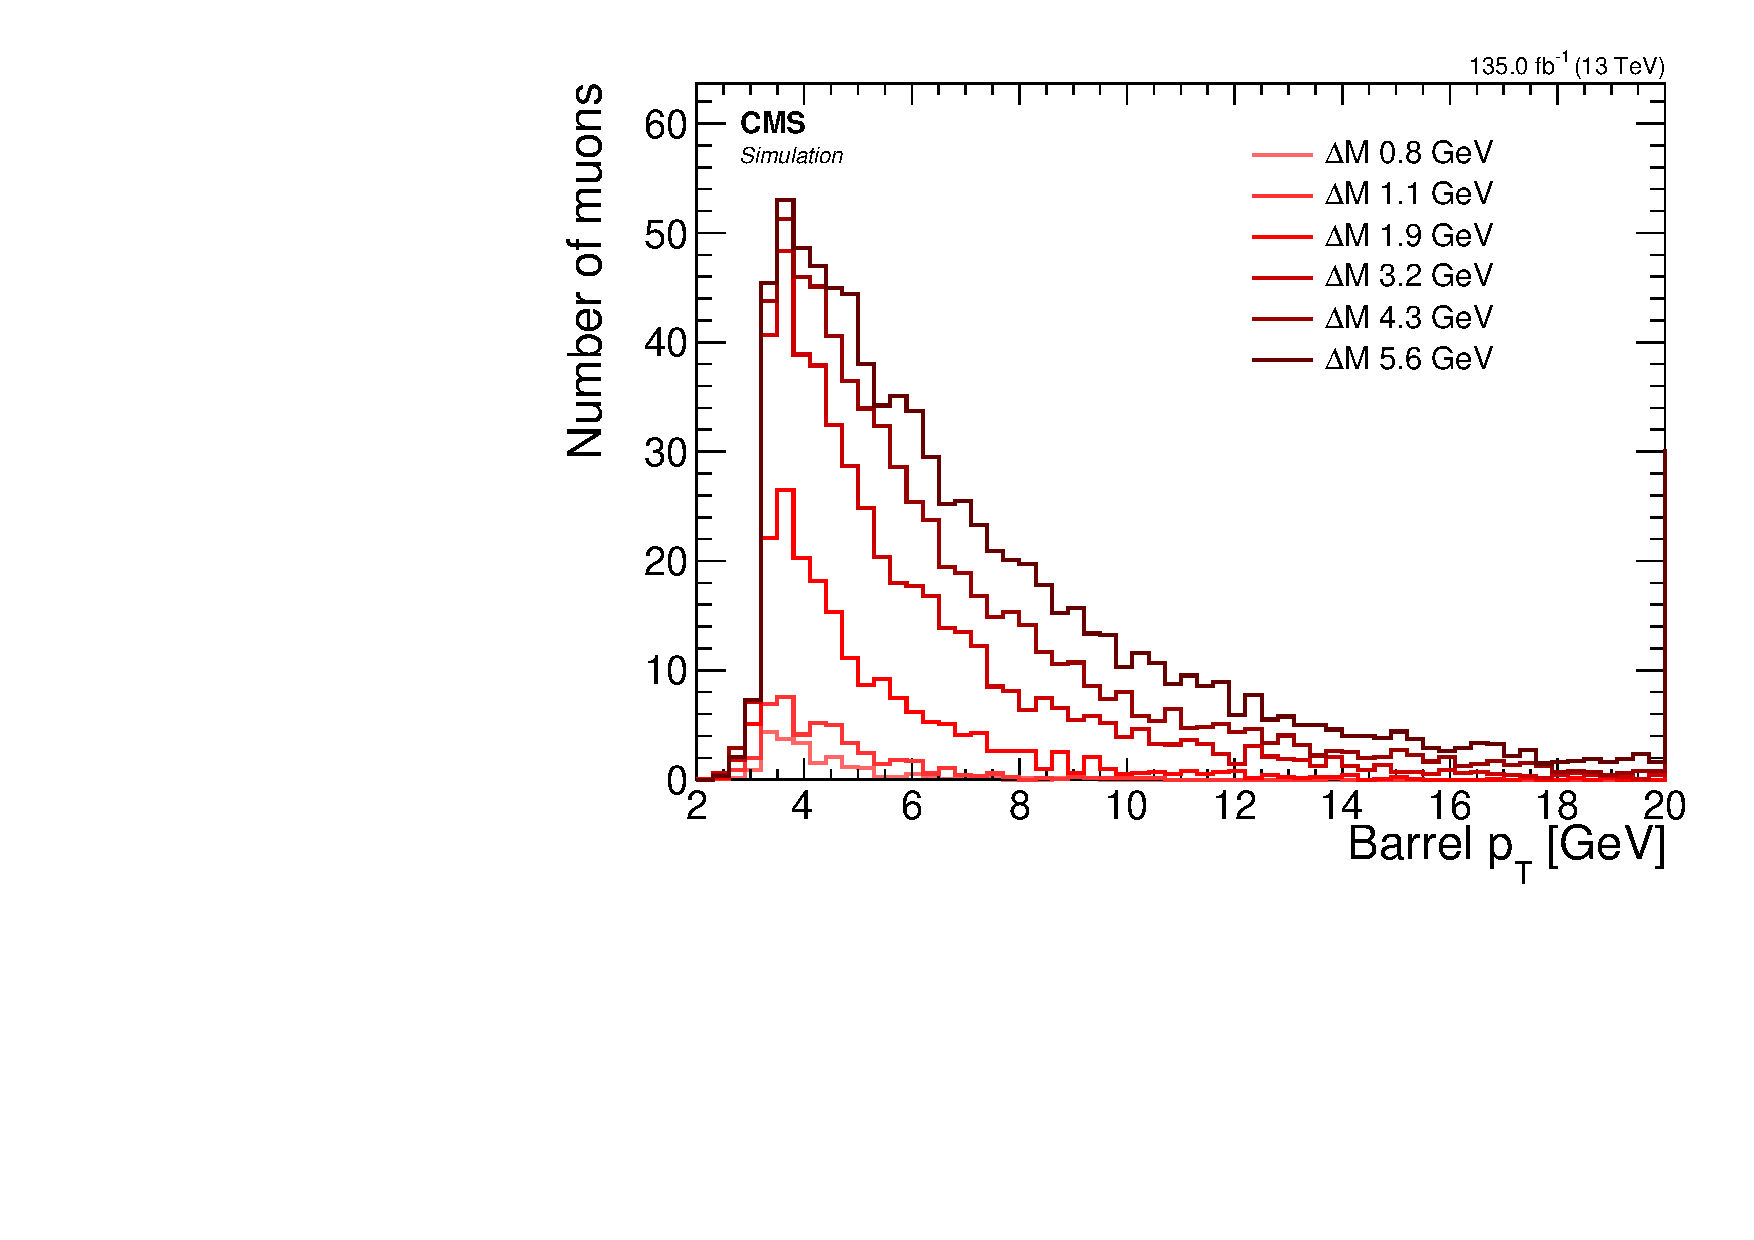
\includegraphics[width=0.48\linewidth]{plots/signal_muons/none_Muons_pt_barrel.pdf} \,
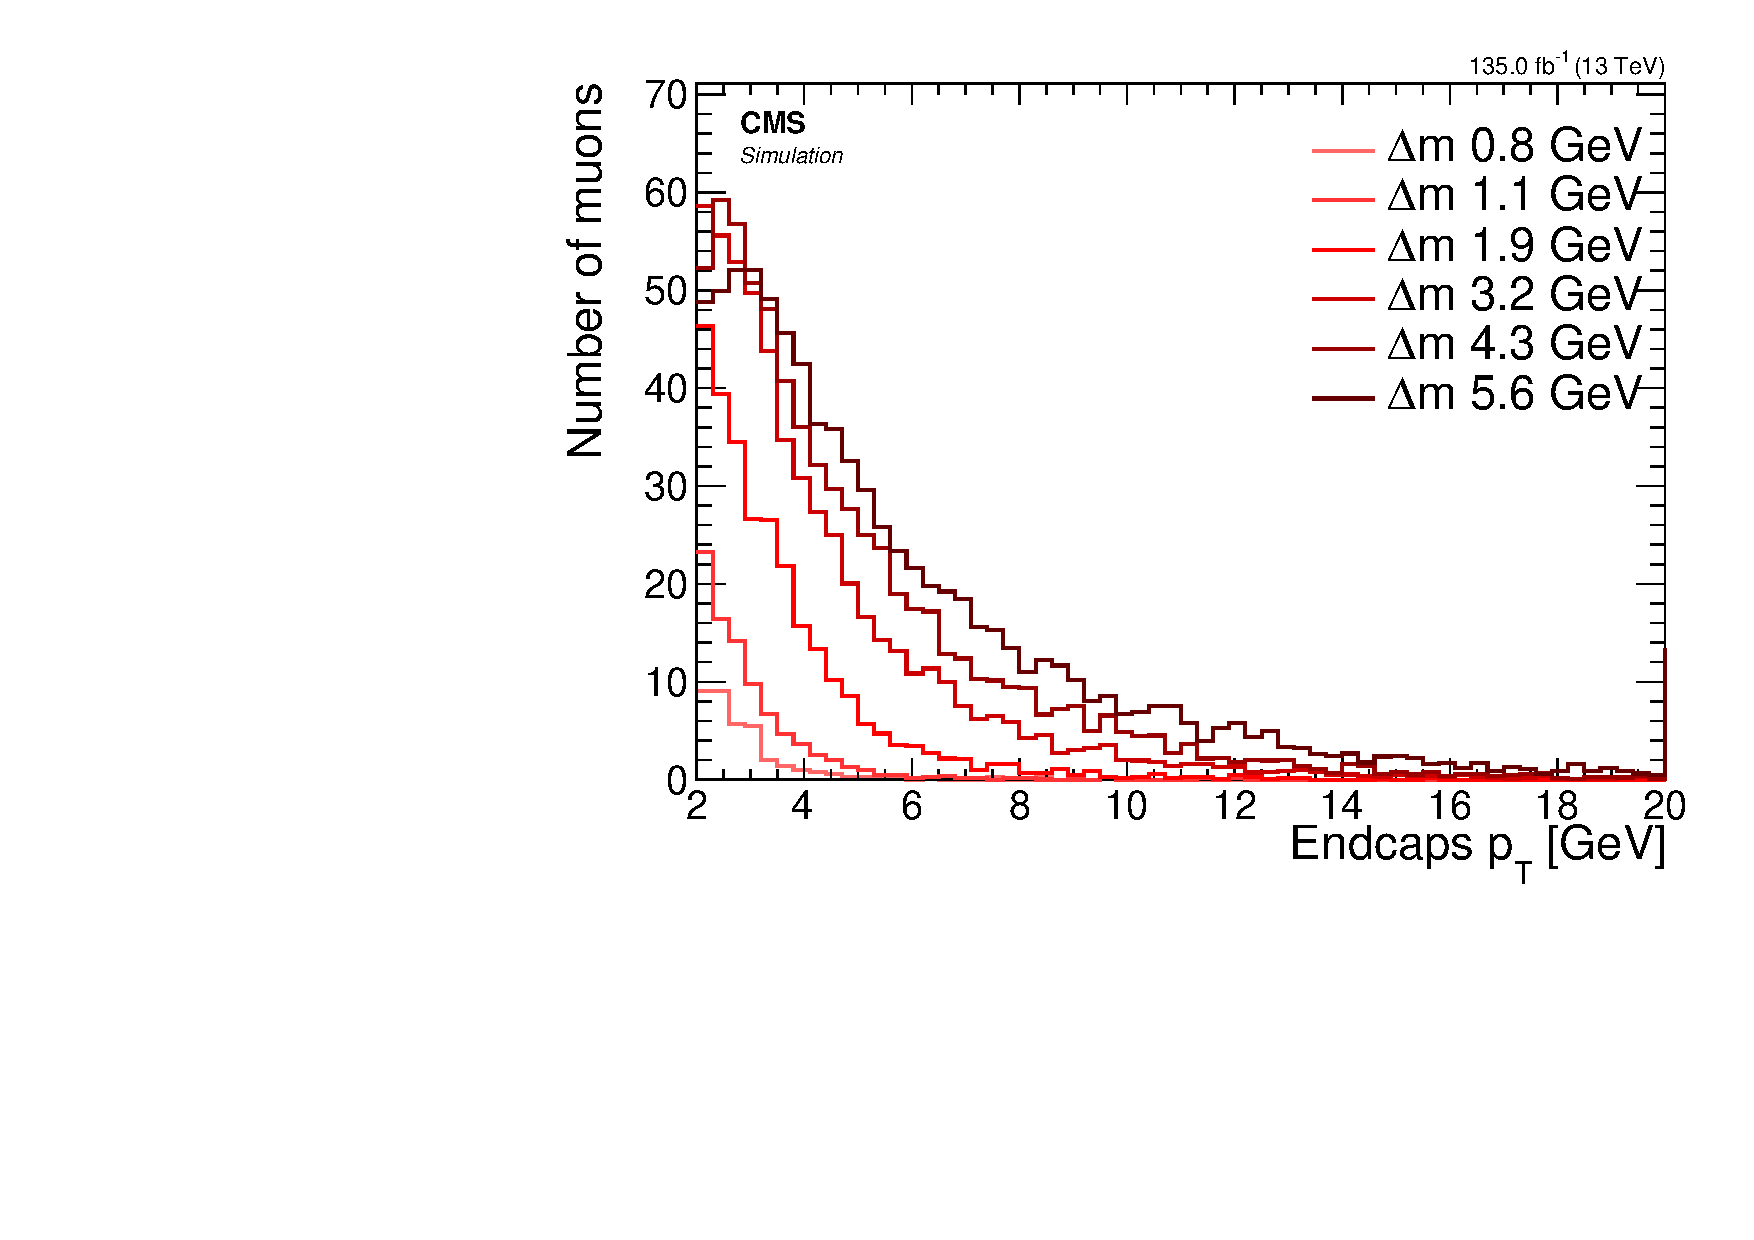
\includegraphics[width=0.48\linewidth]{plots/signal_muons/none_Muons_pt_endcape.pdf}  \\
\caption[Signal \pt distributions split into barrel and endcaps]{ Signal inclusive \pt distributions for barrel $\abs{\eta} < 1.2$ (left) and endcaps $\abs{\eta} \geq 1.2$ (right) at generator level (top) and reconstruction level passing analysis selection (bottom).}
\label{fig:signal-pt-barrel-endcaps}
\end{figure}

When comparing the generator level distribution of the barrel muons on the top left with its reconstructed counterpart on the bottom left, Figure~\ref{fig:signal-pt-barrel-endcaps} shows that the barrel, shown on the left, is almost completely unable to reconstruct muons with $\pt < 3\GeV$, while the endcaps, shown on the right, are able to do so. As demonstrated in the upcoming sections on \gls{mll} and \gls{dr} (see \ref{sec:gen-invariant-mass} and \ref{sec:lepton-dr}), the relationship between these observables has consequences for the reshaping of kinematic distributions, as well as for signal acceptance in general. Access to low \dm signal points is crucially dependent on the low \pt region of $2 \leq \pt \leq 3.5\GeV$, which is mainly achieved with the help of the muon chamber endcaps, as can be seen here.

Since the barrel and endcaps are seperated by different regions of $\eta$, $\abs{\eta} < 1.2$ for barrel and $\abs{\eta} \geq 1.2$ for endcaps, the muon $\eta$ distributions merit further examination as well. They can be seen at Figure~\ref{fig:signal-muons-eta}. The dimuon analysis channel only selects muons within the tracker range of $\abs{\eta}<2.4$. This is why the muons with $\abs{\eta}>2.4$ are not present in the reconstruction plots on the bottom. It can be seen that the main effect of going from the inclusive $\abs{\eta}$ at the generator level to the reconstructed counterpart is the flattening of the distribution due to the loss of muons with $\abs{\eta}<1.2$ in the barrel for muons with $\pt<3\GeV$.

\begin{figure}[!htb]
\centering
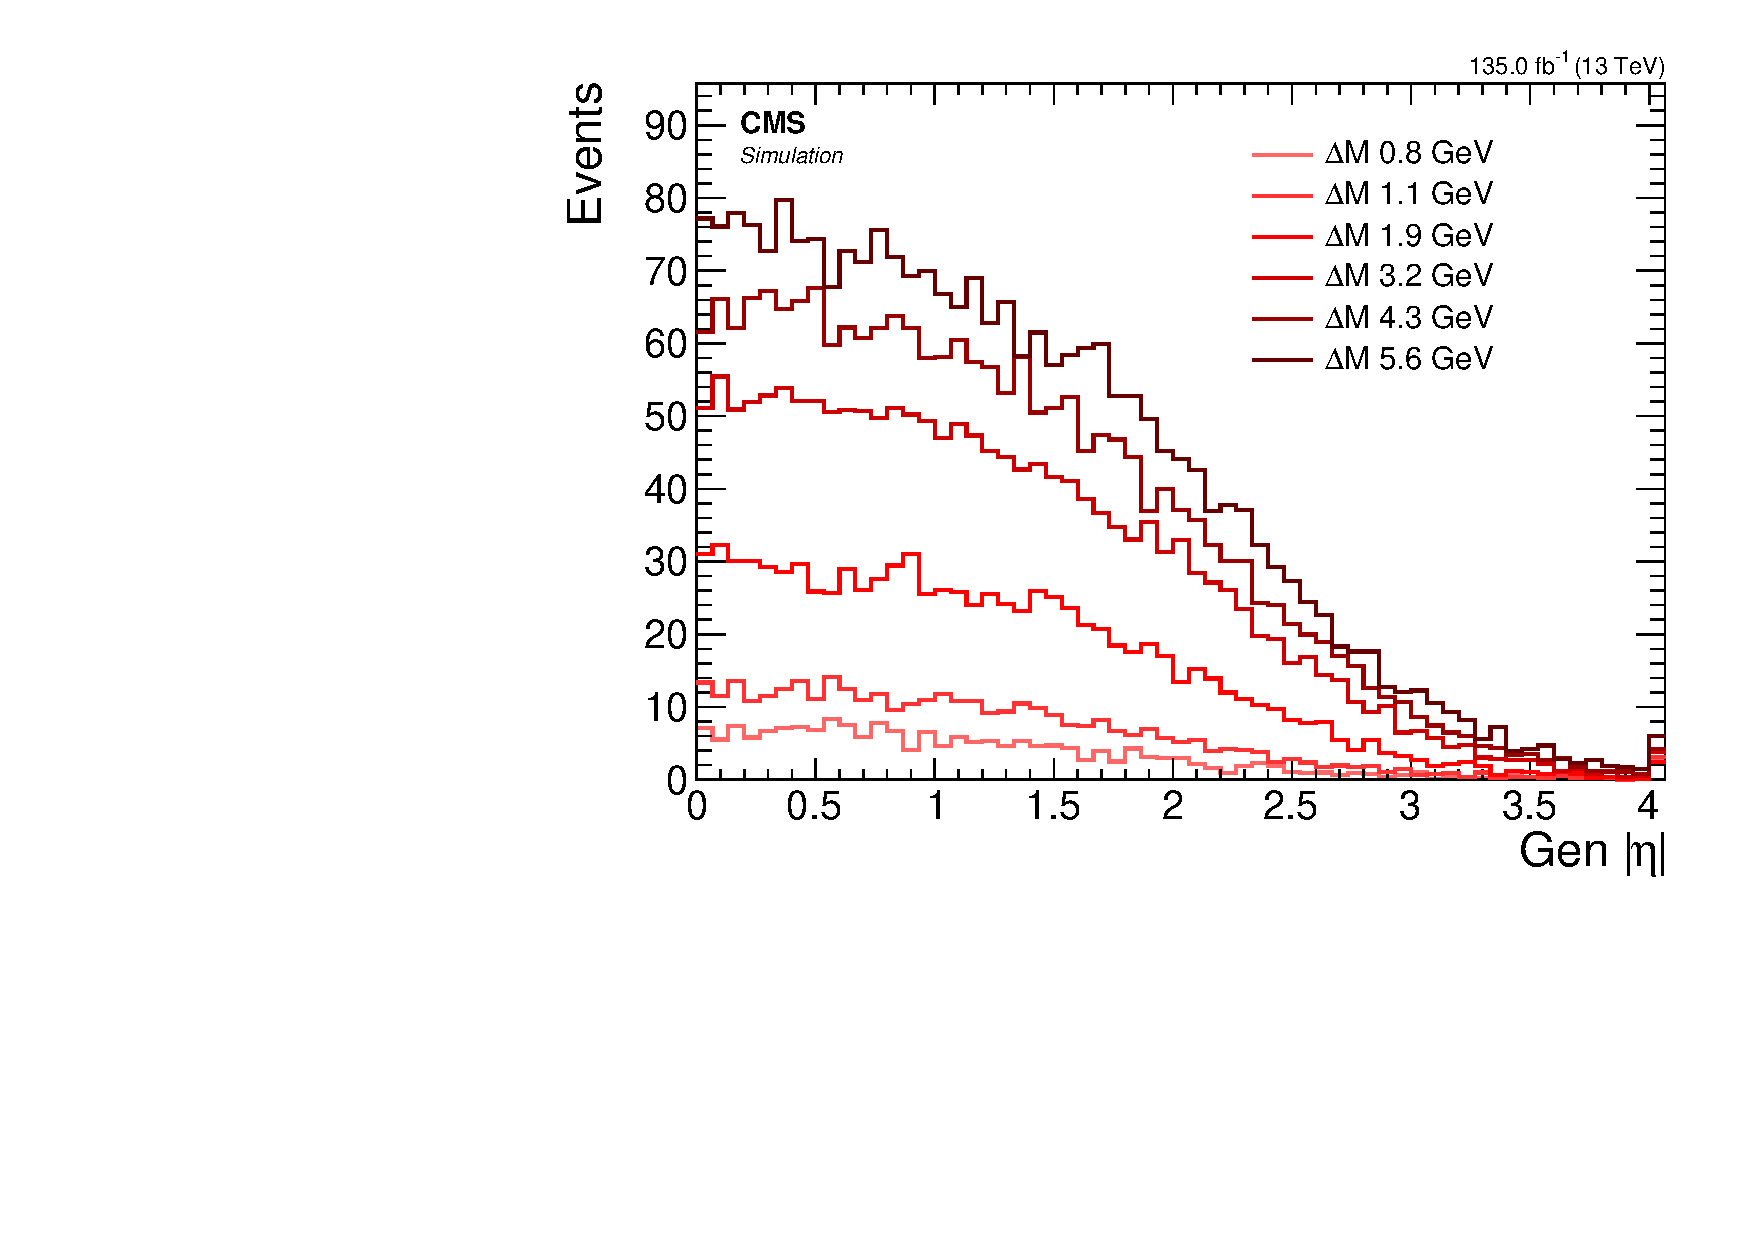
\includegraphics[width=0.32\linewidth]{plots/signal_muons_gen/none_Muons_Eta.pdf} \,
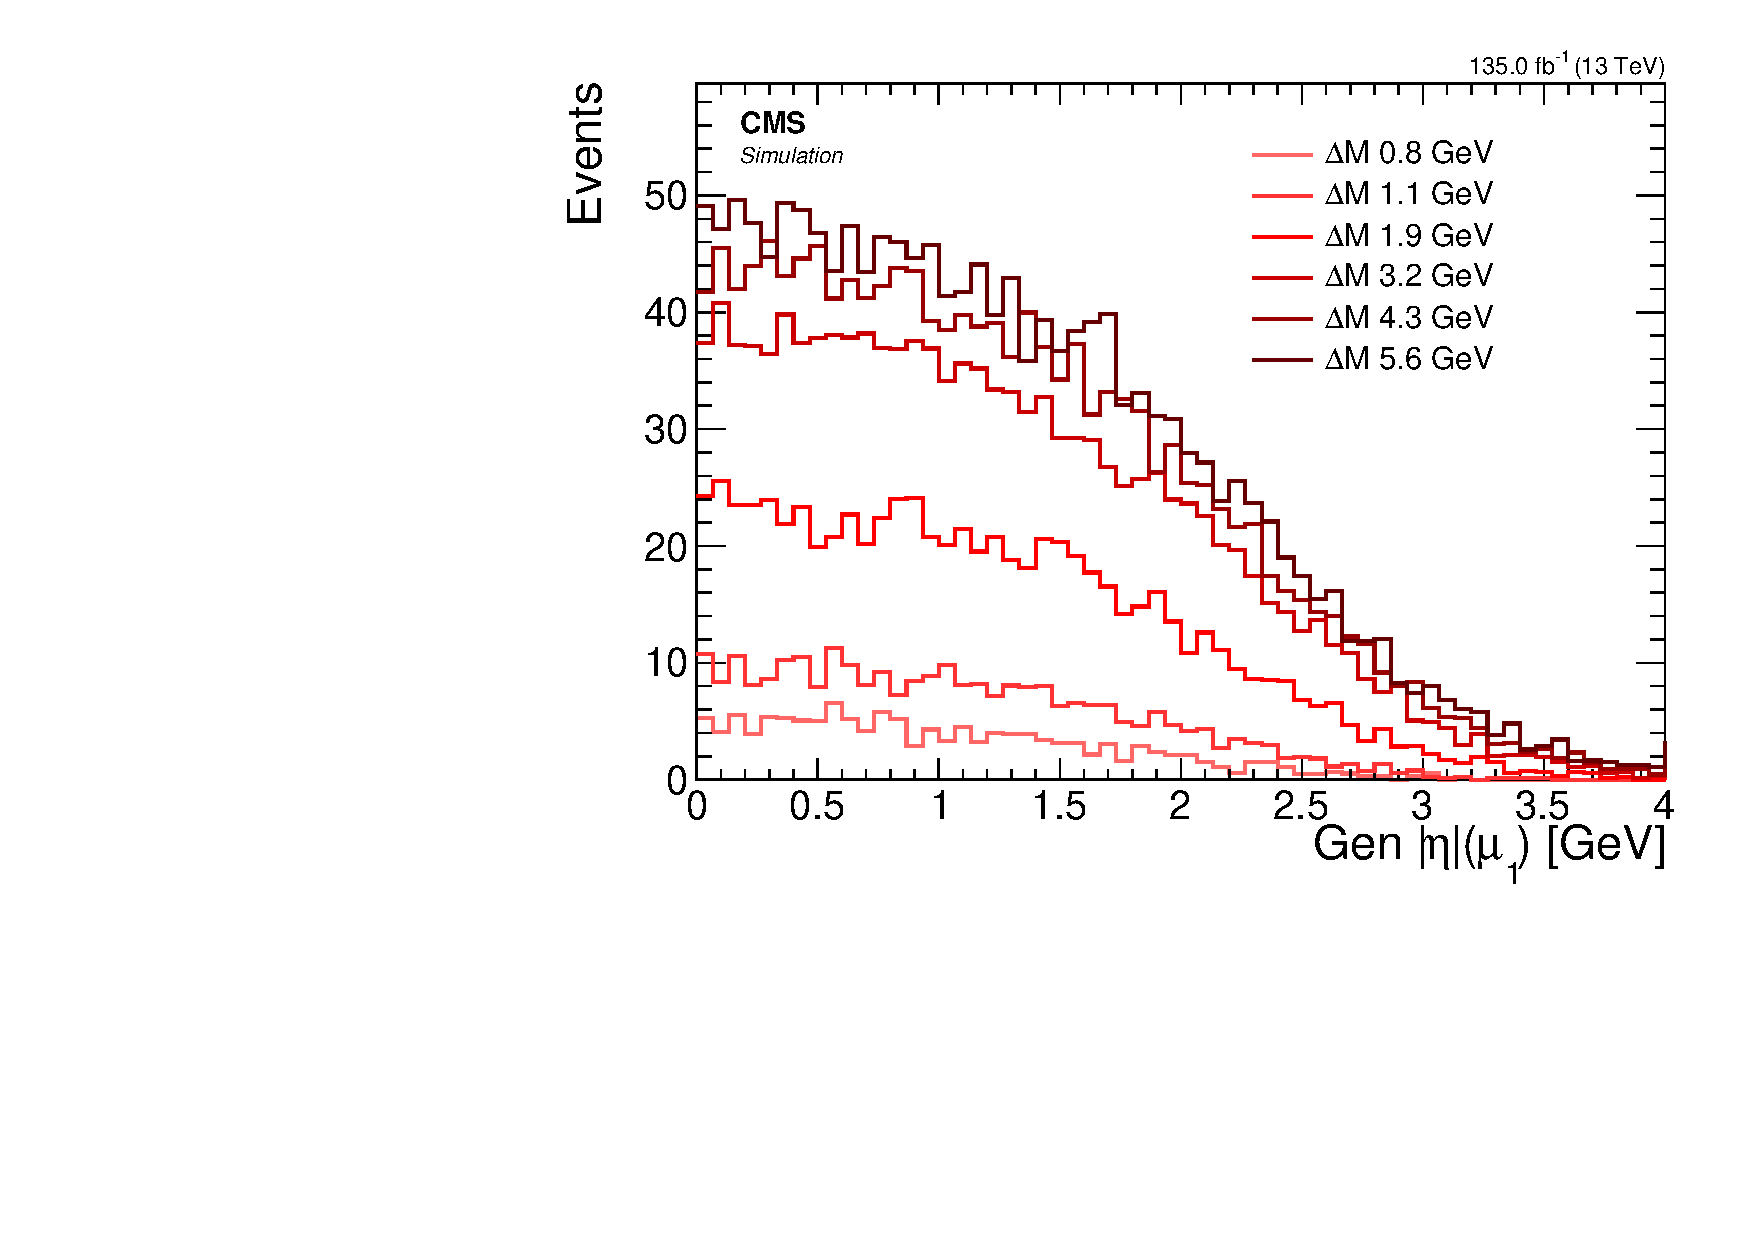
\includegraphics[width=0.32\linewidth]{plots/signal_muons_gen/none_Muons_m1_eta.pdf}  \,
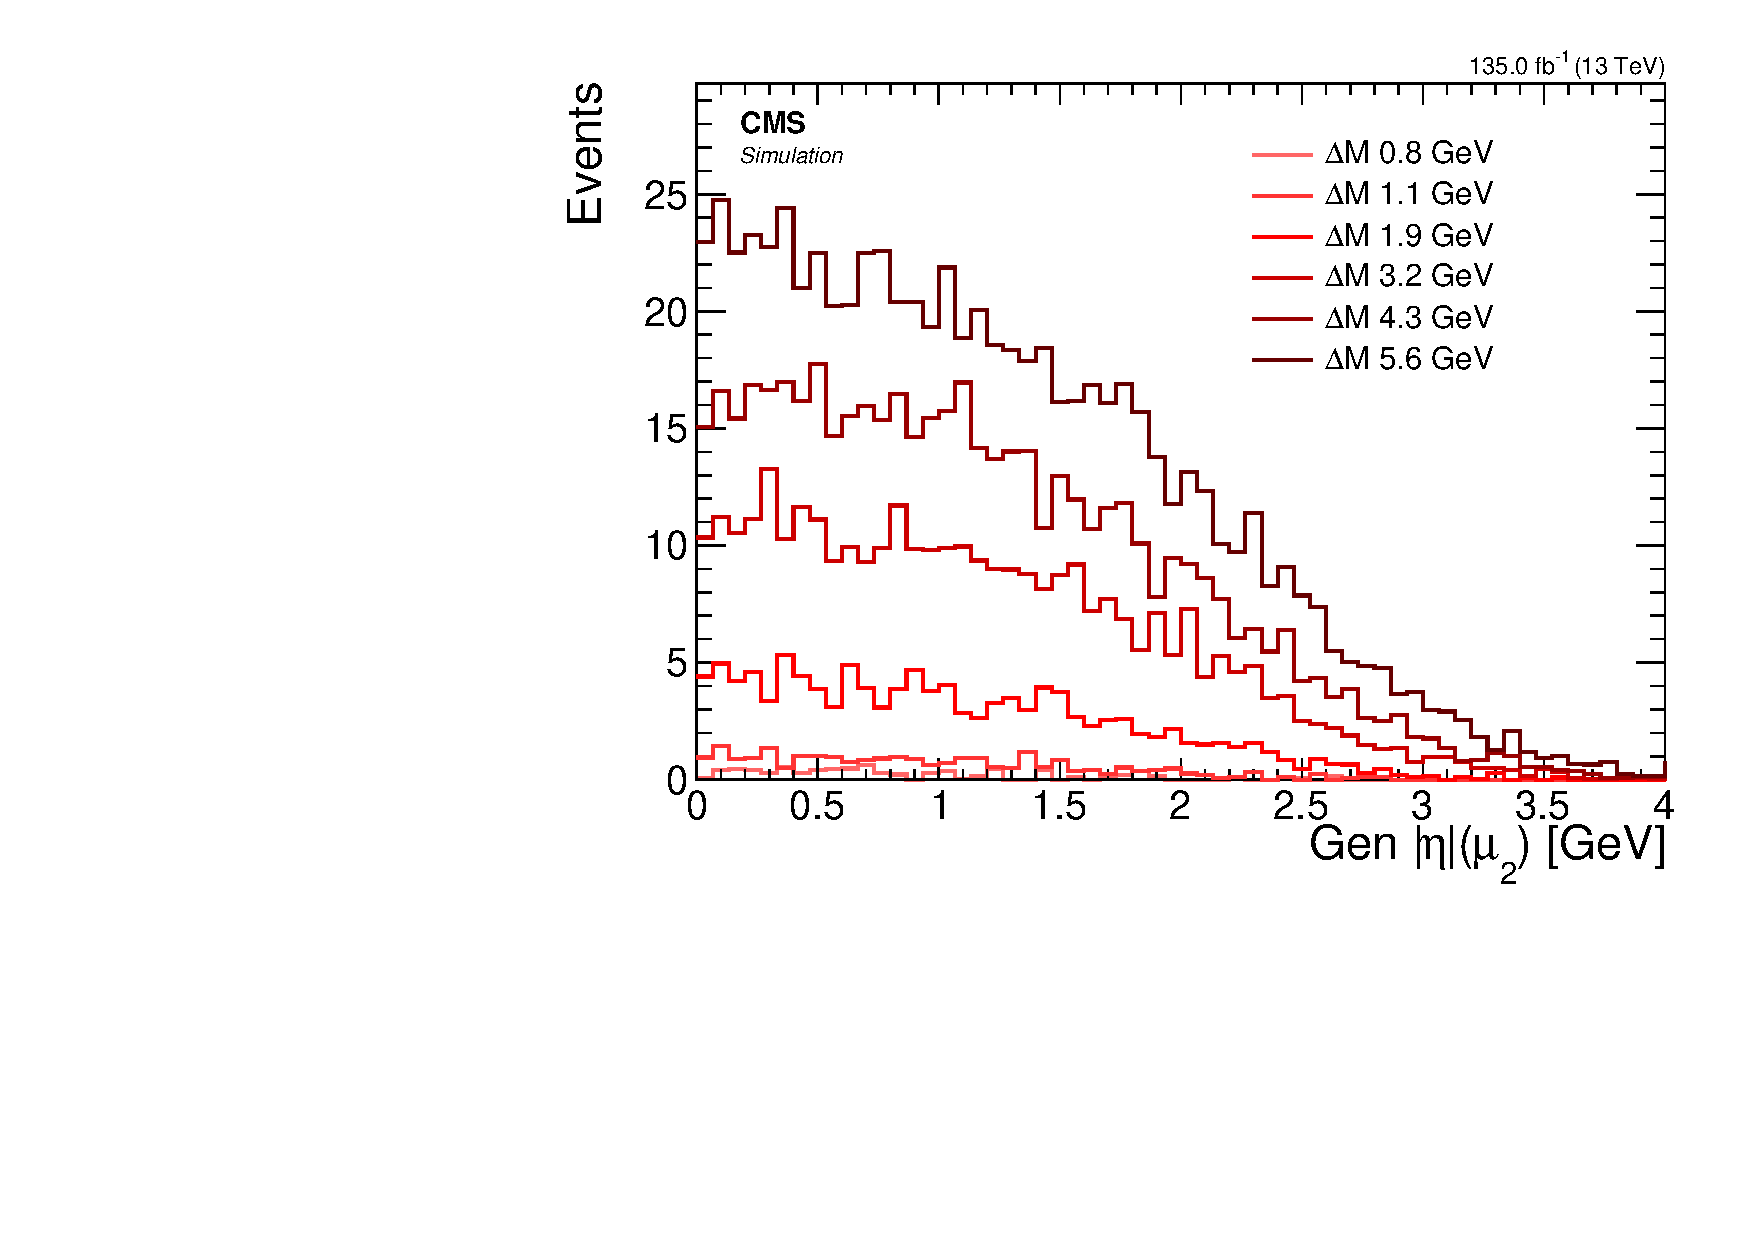
\includegraphics[width=0.32\linewidth]{plots/signal_muons_gen/none_Muons_m2_eta.pdf} \\
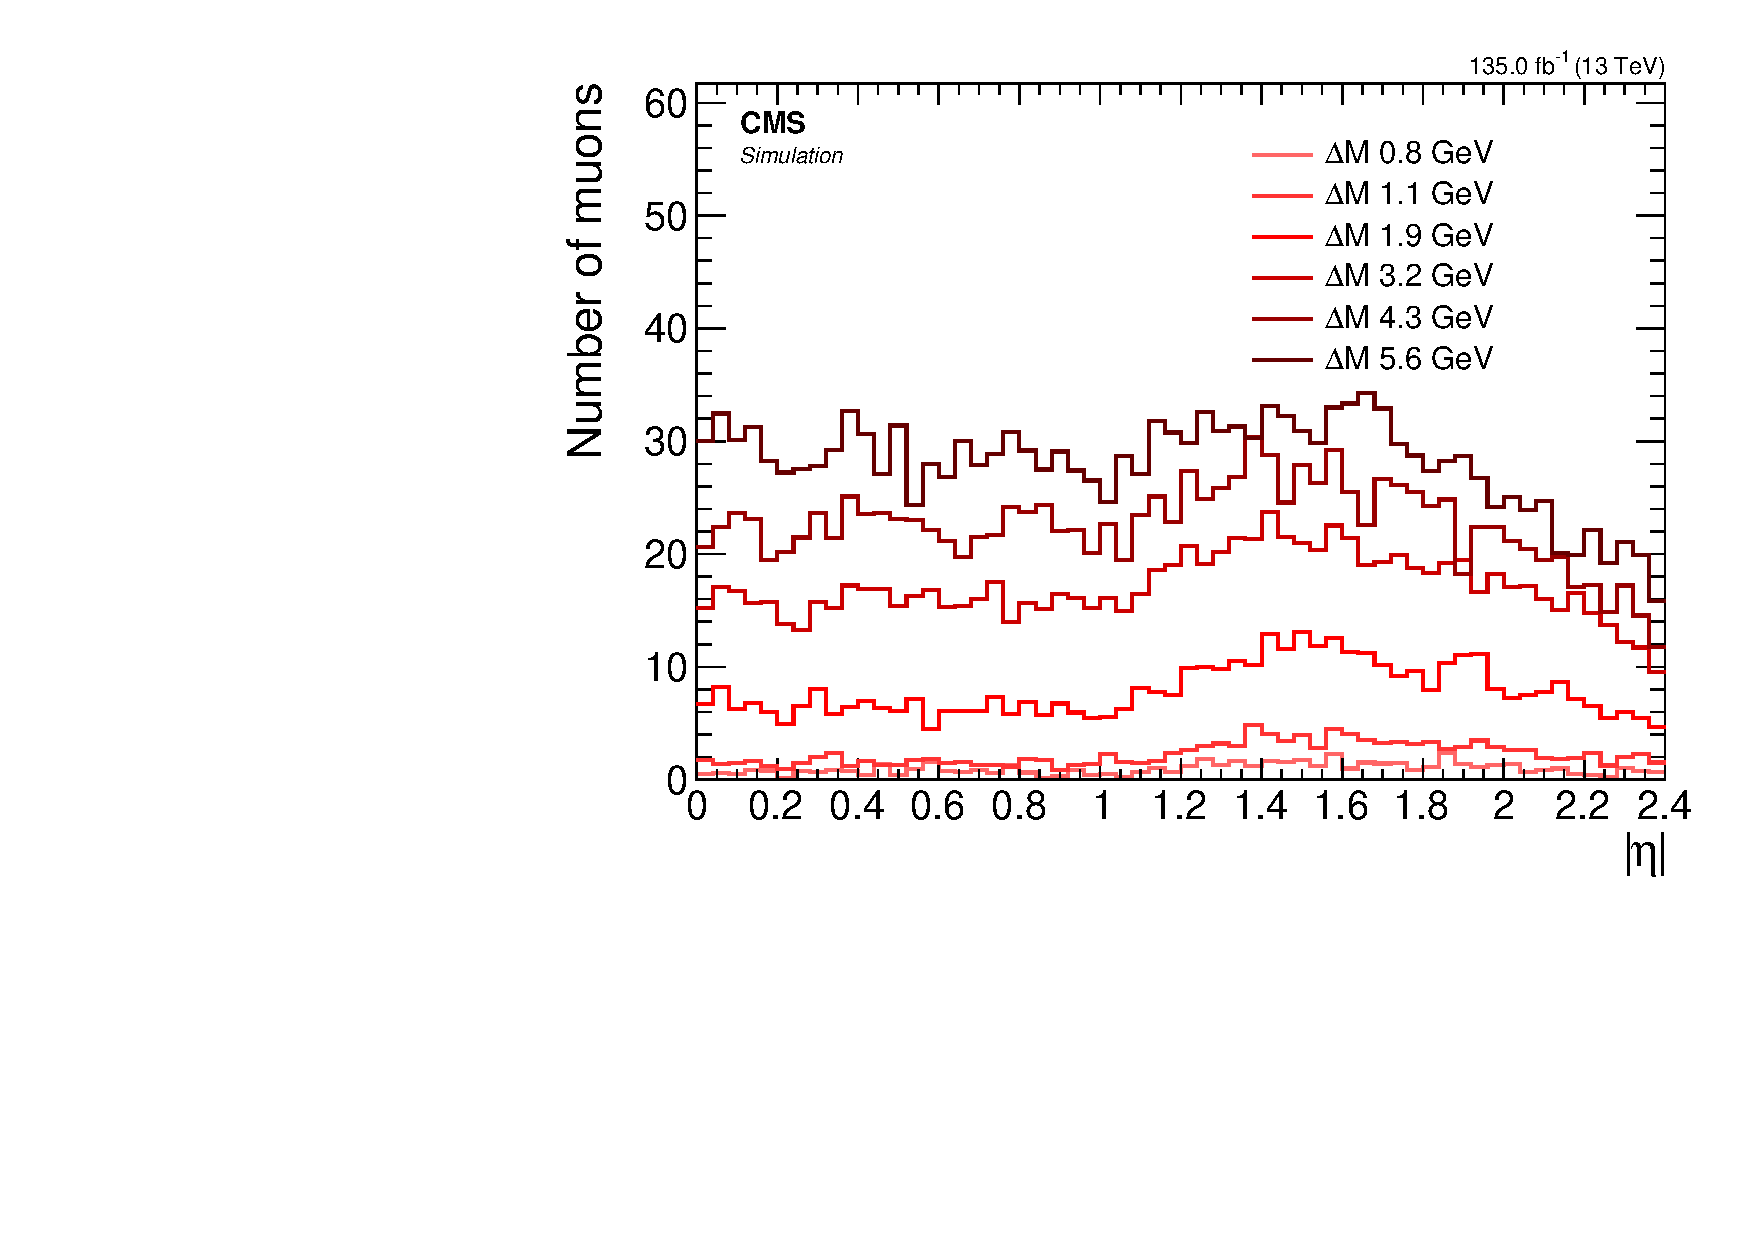
\includegraphics[width=0.32\linewidth]{plots/signal_muons/none_Muons_Eta.pdf} \,
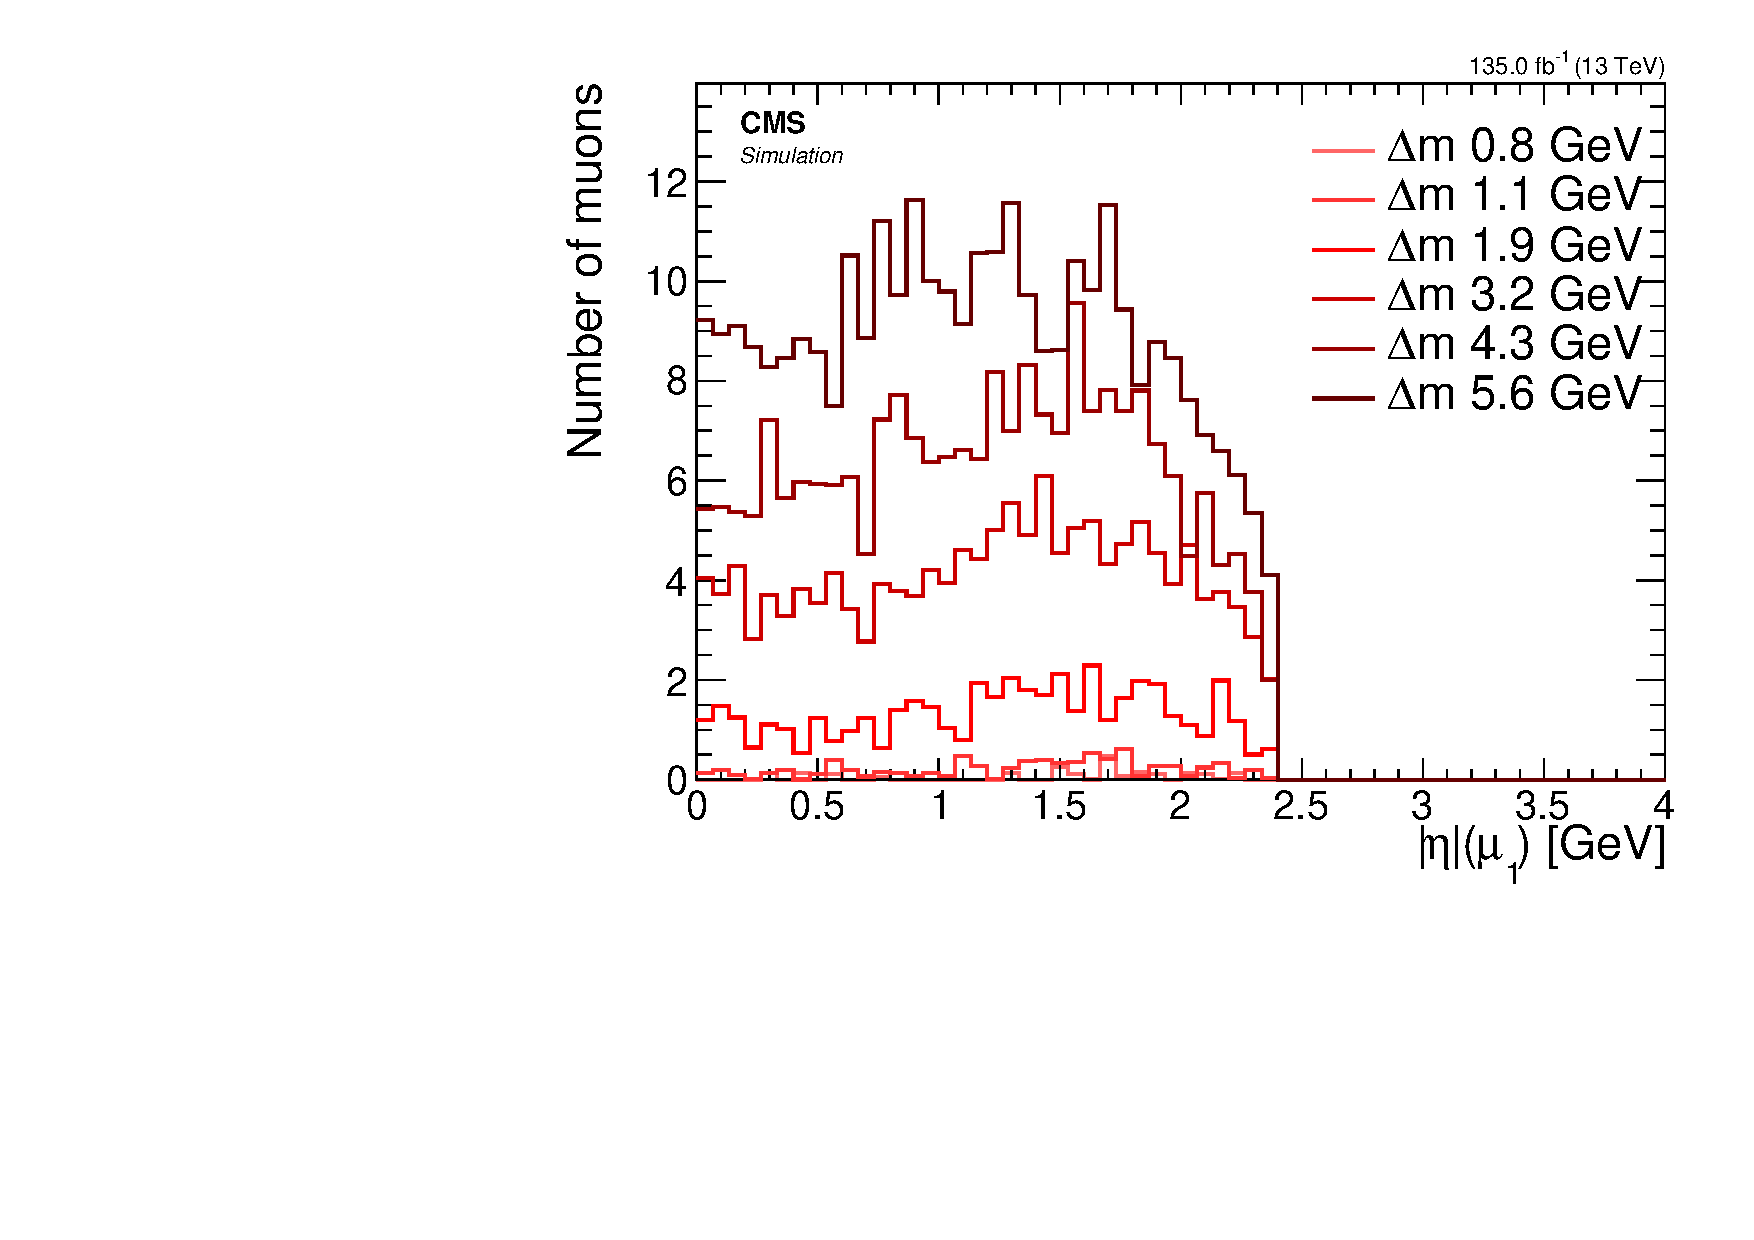
\includegraphics[width=0.32\linewidth]{plots/signal_muons/none_Muons_m1_eta.pdf}  \,
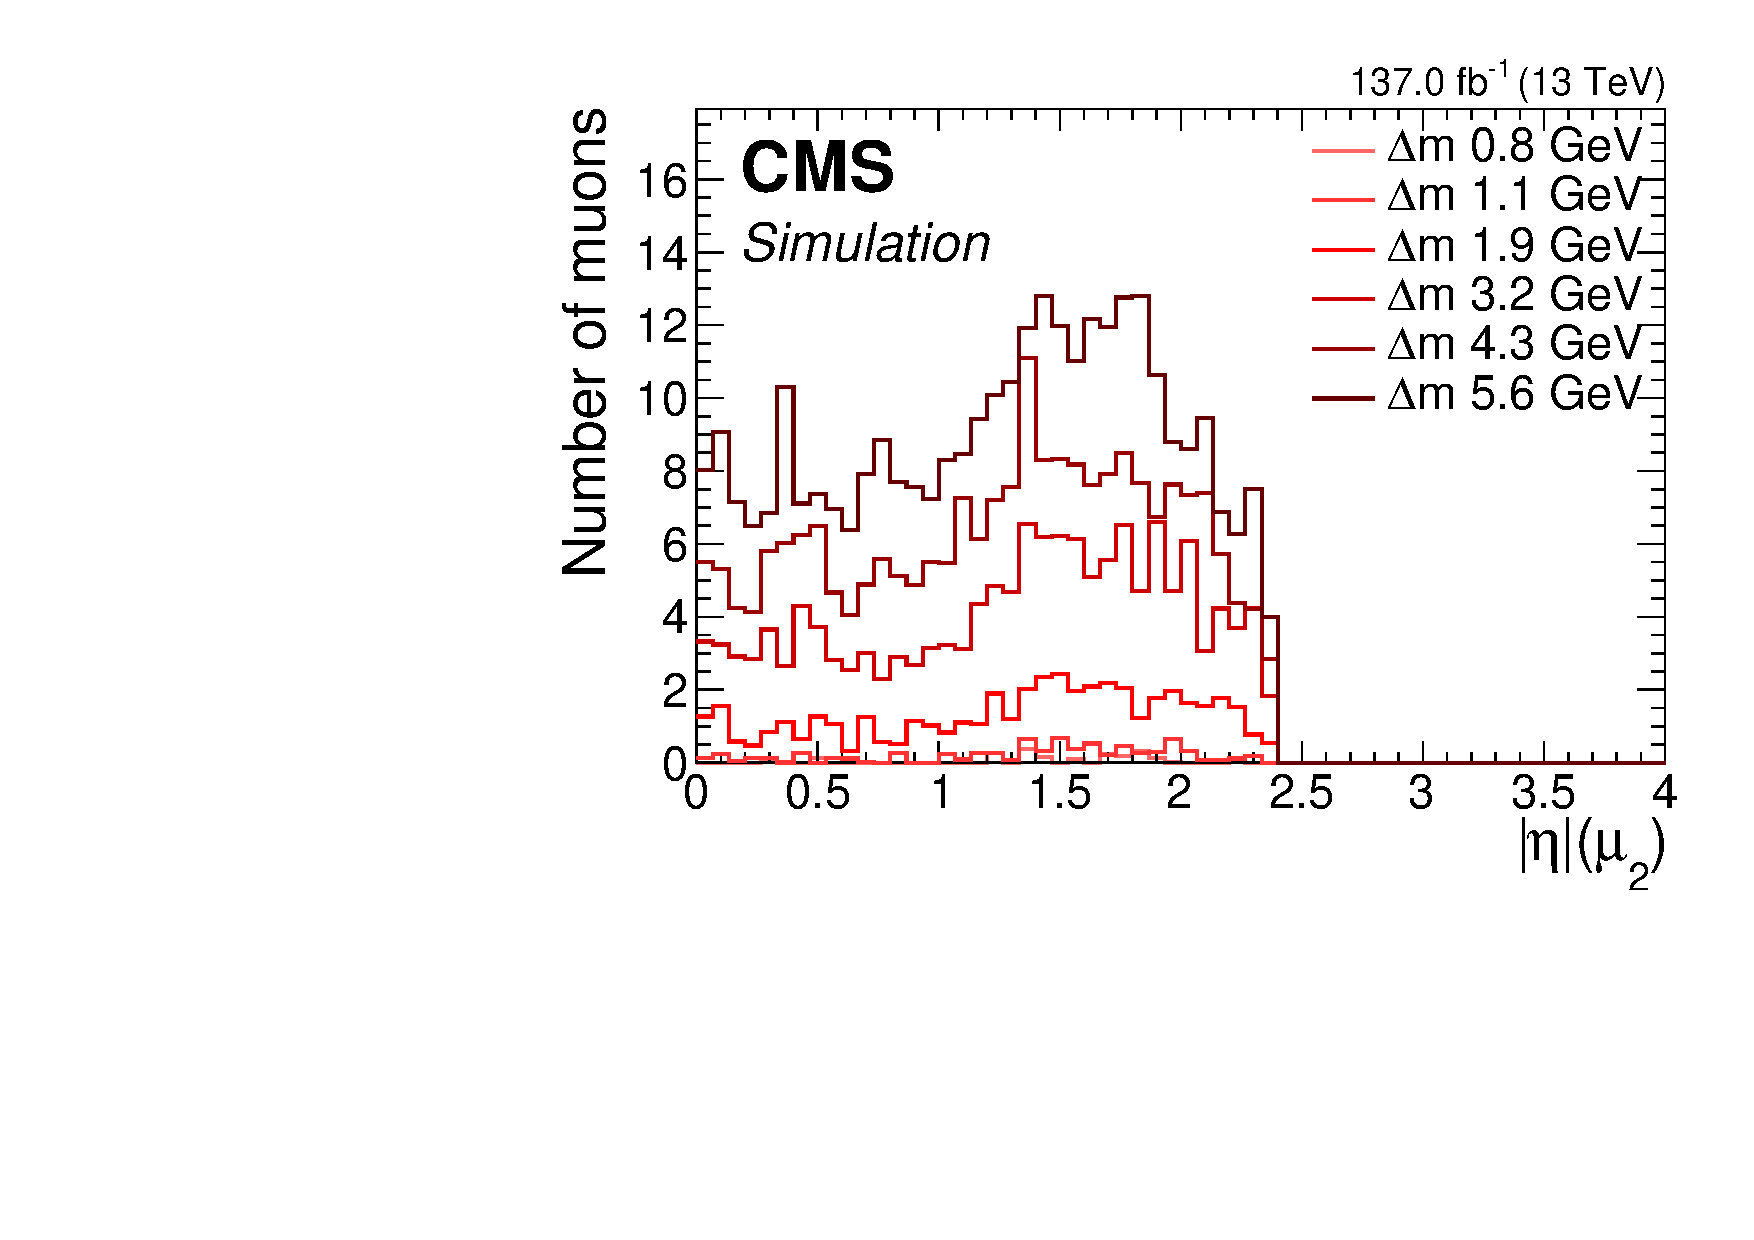
\includegraphics[width=0.32\linewidth]{plots/signal_muons/none_Muons_m2_eta.pdf} \\
\caption[Signal $\abs{\eta}$ distributions]{ Signal $\abs{\eta}$ distributions for inclusive (left), leading muon $\mu_1$ (middle),  subleading muon $\mu_2$ (right) at generator level (top) and reconstruction level passing analysis selection (bottom). }
\label{fig:signal-muons-eta}
\end{figure}

With the understanding of the reconstruction effects on the \pt and $\eta$ distributions of the muons, an examination of other kinematic variables of the dilepton system is now possible.

\clearpage

\subsubsection{Invariant mass \gls{mll}}
\label{sec:gen-invariant-mass}

The invariant mass of the two leptons resulting from the decay of the \neutt has a unique shape due to the limited allowed phase space of the 3-body decay. As the \neutt decays into \neuto and \ellell through a \PZstar, the allowed phase space of the dilepton pair is restricted to the mass difference between \neutt and \neuto, that is, \dm. Therefore, the \gls{mll} distribution is expected to have an edge at \dm. Distributions of the generator level invariant mass can be seen in Figure~\ref{fig:signal-generator-mll}.

\begin{figure}[!htb]
\centering
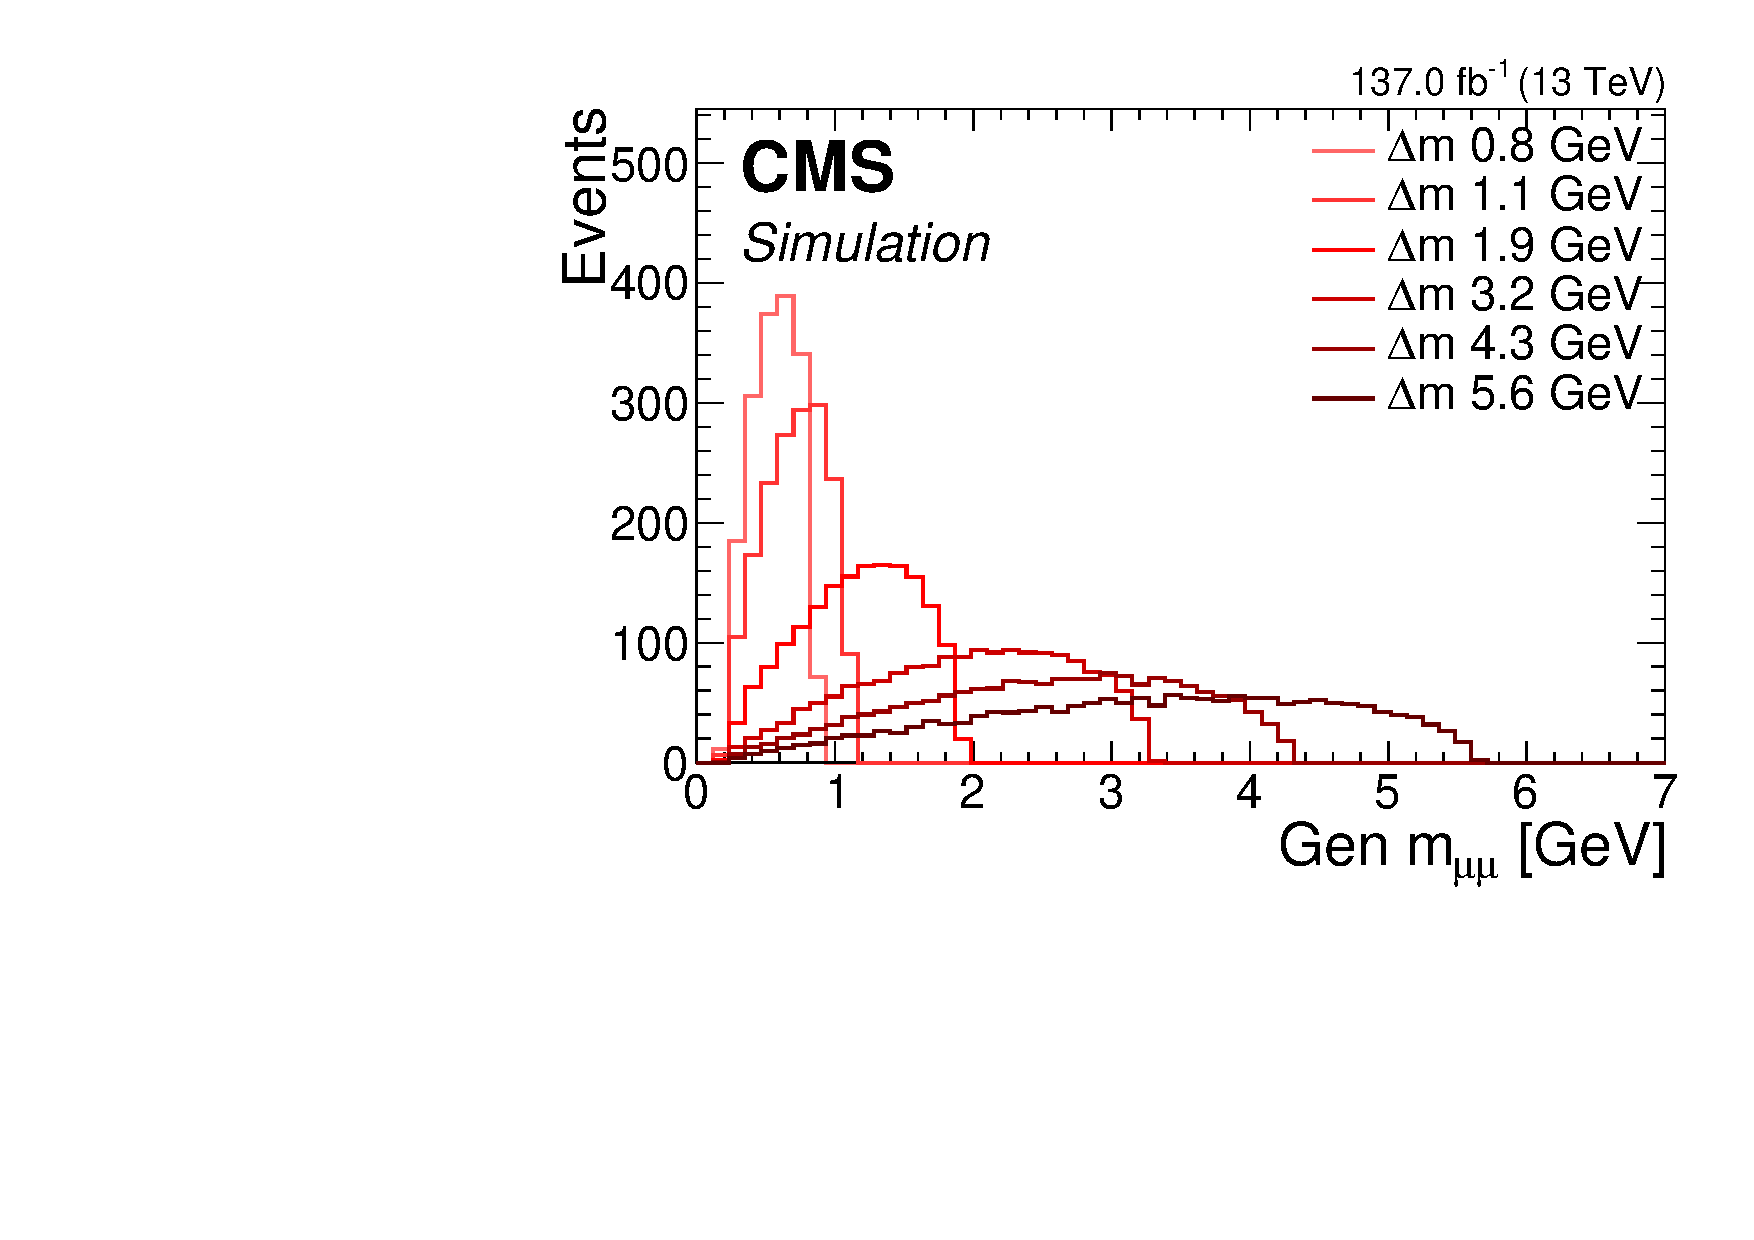
\includegraphics[width=0.32\linewidth]{plots/signal_muons_gen/none_gen_invMass.pdf} \,
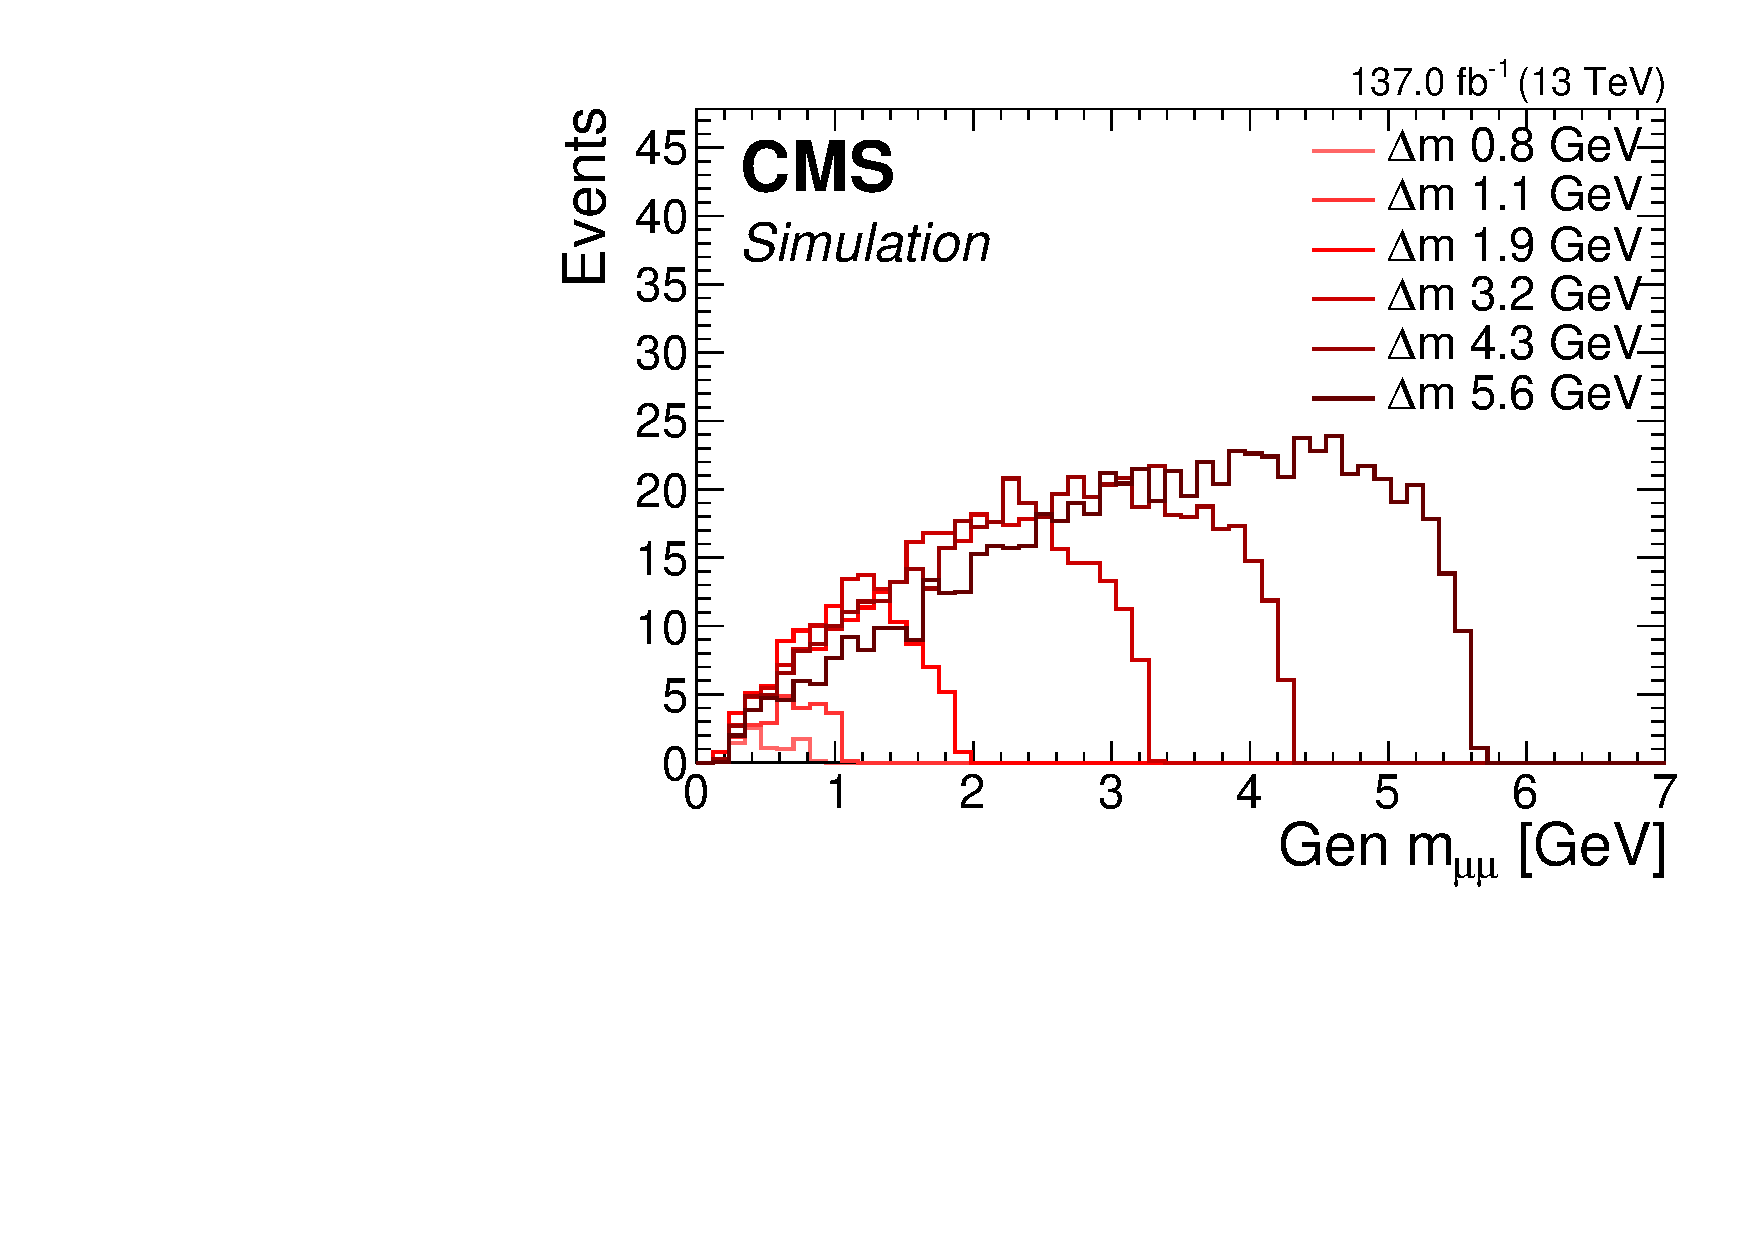
\includegraphics[width=0.32\linewidth]{plots/signal_muons_gen/none_gen_invMass_cut.pdf}  \,
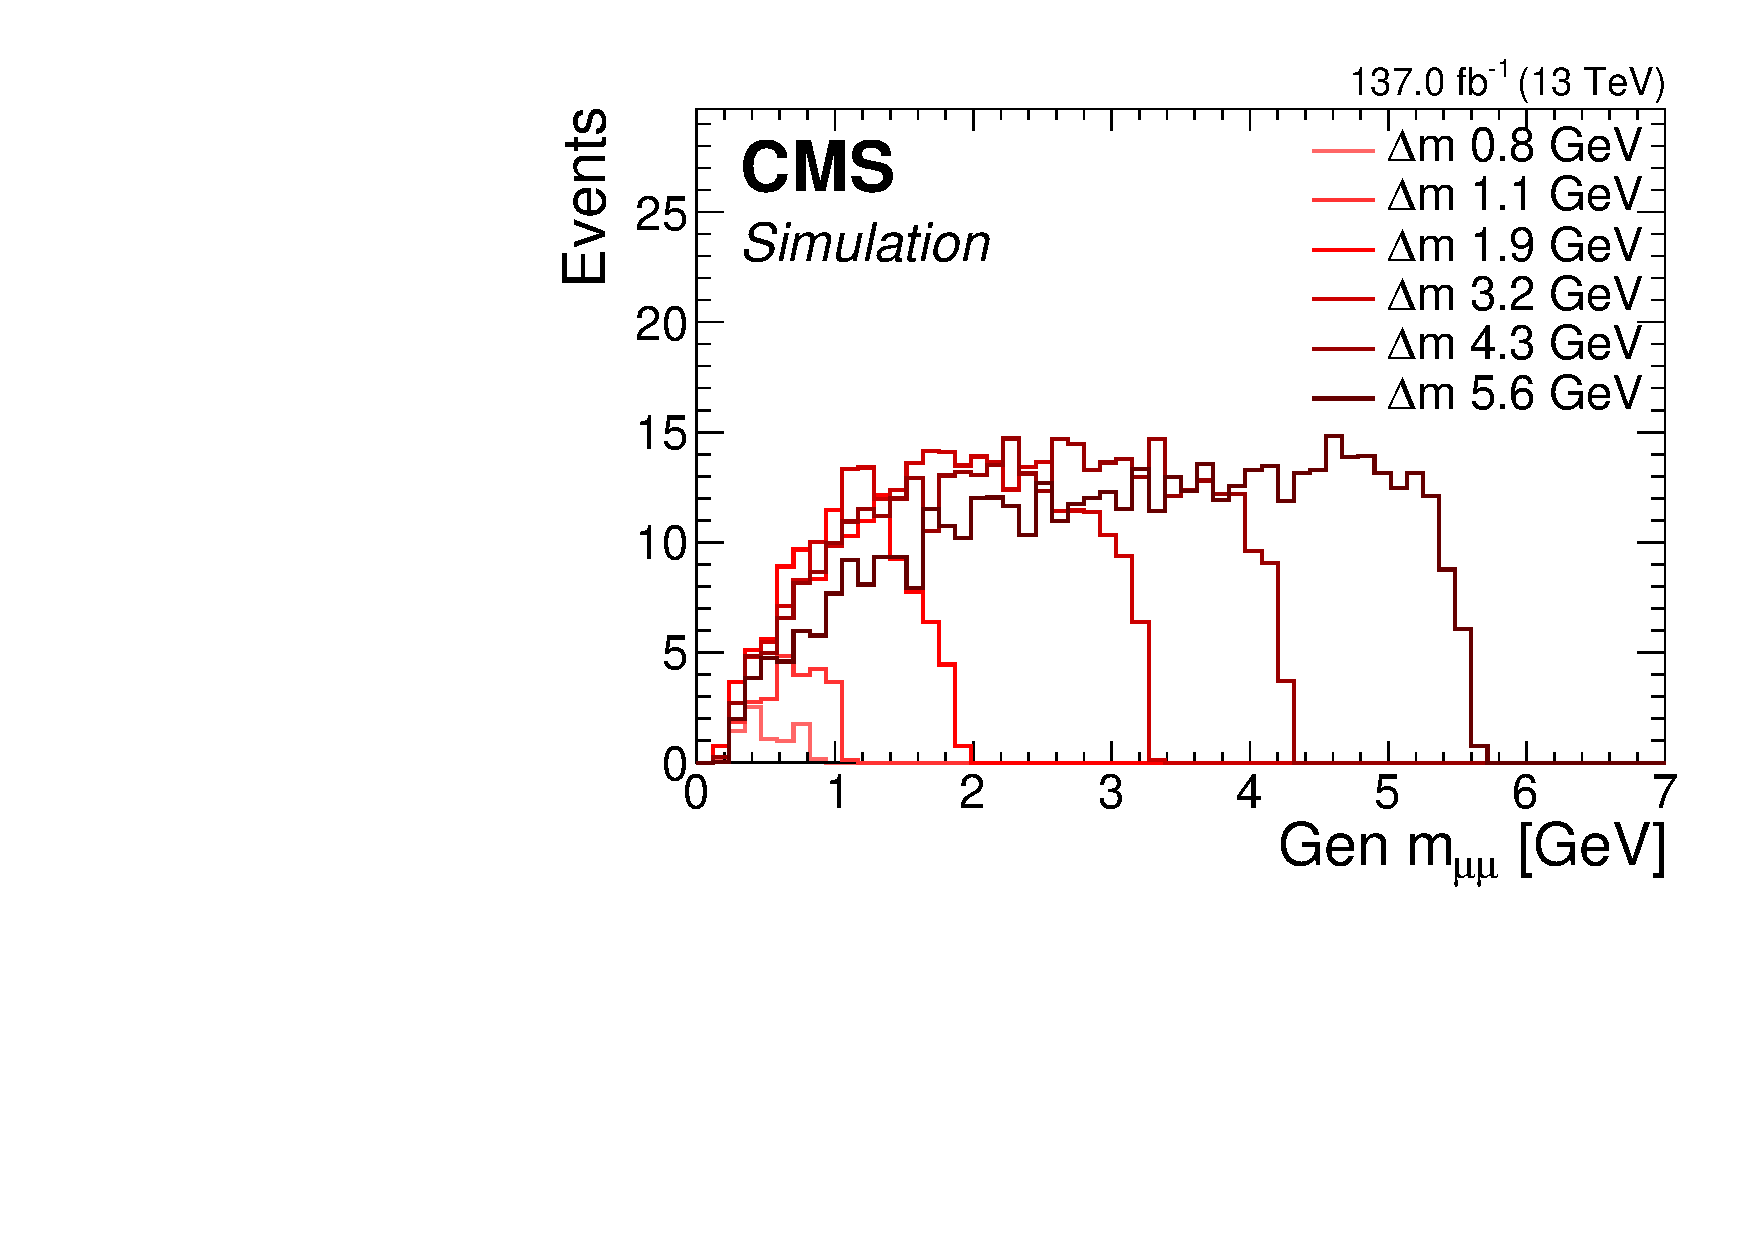
\includegraphics[width=0.32\linewidth]{plots/signal_muons_gen/none_gen_invMass_orth.pdf} \\
\caption[Signal generator level \mll distributions]{ Signal generator level \mll distributions with no cuts (left), with $\pt\left(\mu_i\right)>2\GeV,\,i=1,2$ (middle) and with the \gls{sos} orthogonality condition: $\pt\left(\mu_i\right)>2\GeV$, $\pt\left(\mu_2\right)\leq~3.5\GeV\text{ or }\Delta R\leq 0.3$ (right).}
\label{fig:signal-generator-mll}
\end{figure}

The inclusive distribution of the invariant mass of the muons \mmumu is shown on the left. The edge of the \mmumu distribution for each signal point is located right at the corresponding \dm. However, when the muons \pt is required to be $\pt\geq 2\GeV$, the shape of the distribution shifts, due to the lower efficiency for small \dm values, as depicted in the middle plot. Lastly, the effect of orthogonalizing phase space to the \gls{sos} analysis is demonstrated in the rightmost plot. The effect is strongest in high \dm and quite subtle in low \dm.

To explain the reshaping that occurs to the \mmumu distribution, the relationship between the \pt of the muons and the invariant mass is examined. One signal with low \dm of $1.13\GeV$ and one with high \dm of $5.63\GeV$ are selected for this analysis. The distributions are shown in Figure~\ref{fig:signal-gen-invamass-pt}, leading muon denoted $\mu_1$ while subleading muon is denoted $\mu_2$.

\begin{figure}[!htb]
\centering
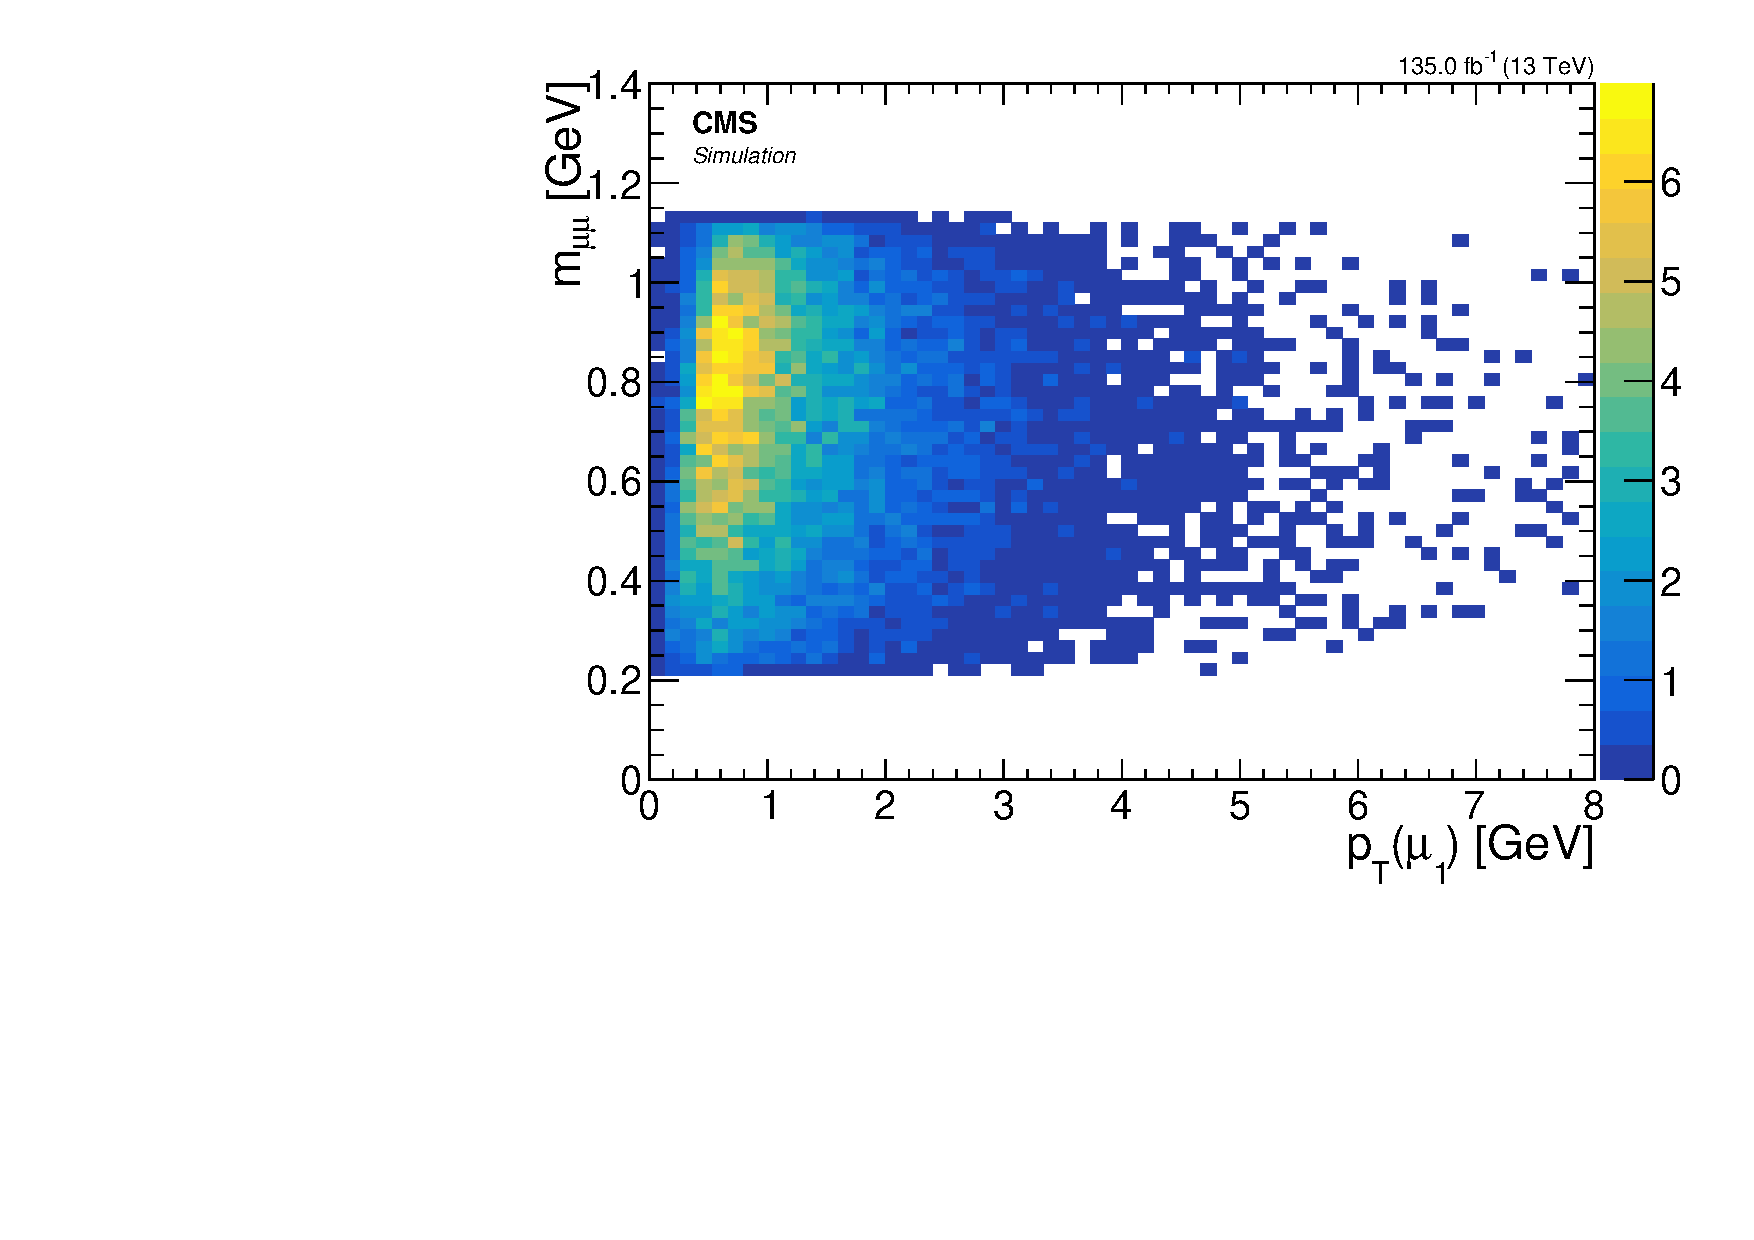
\includegraphics[width=0.48\linewidth]{plots/signal_muons_gen_delta_r_vs_pt/none_gen_invmass_vs_pt_1.pdf} \,
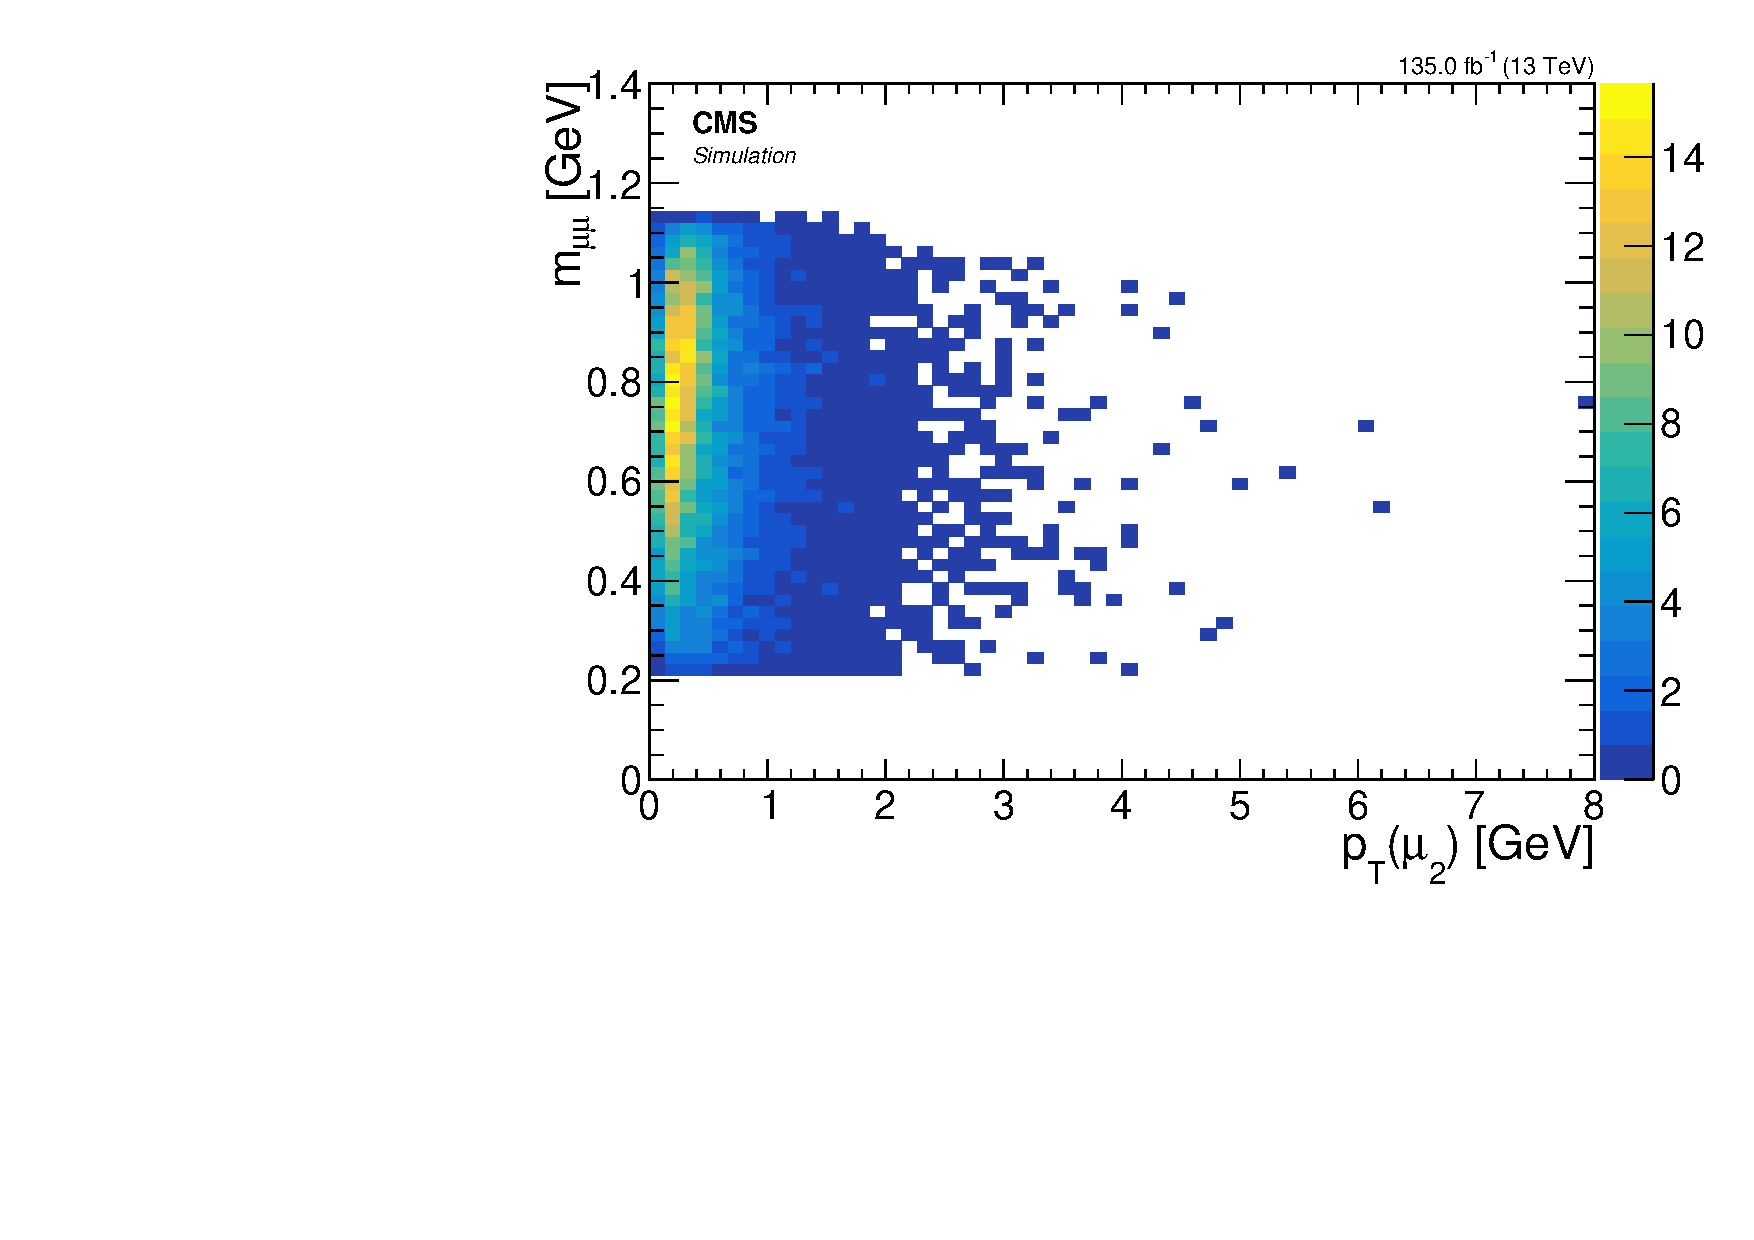
\includegraphics[width=0.48\linewidth]{plots/signal_muons_gen_delta_r_vs_pt/none_gen_invmass_vs_pt_2.pdf}  \\
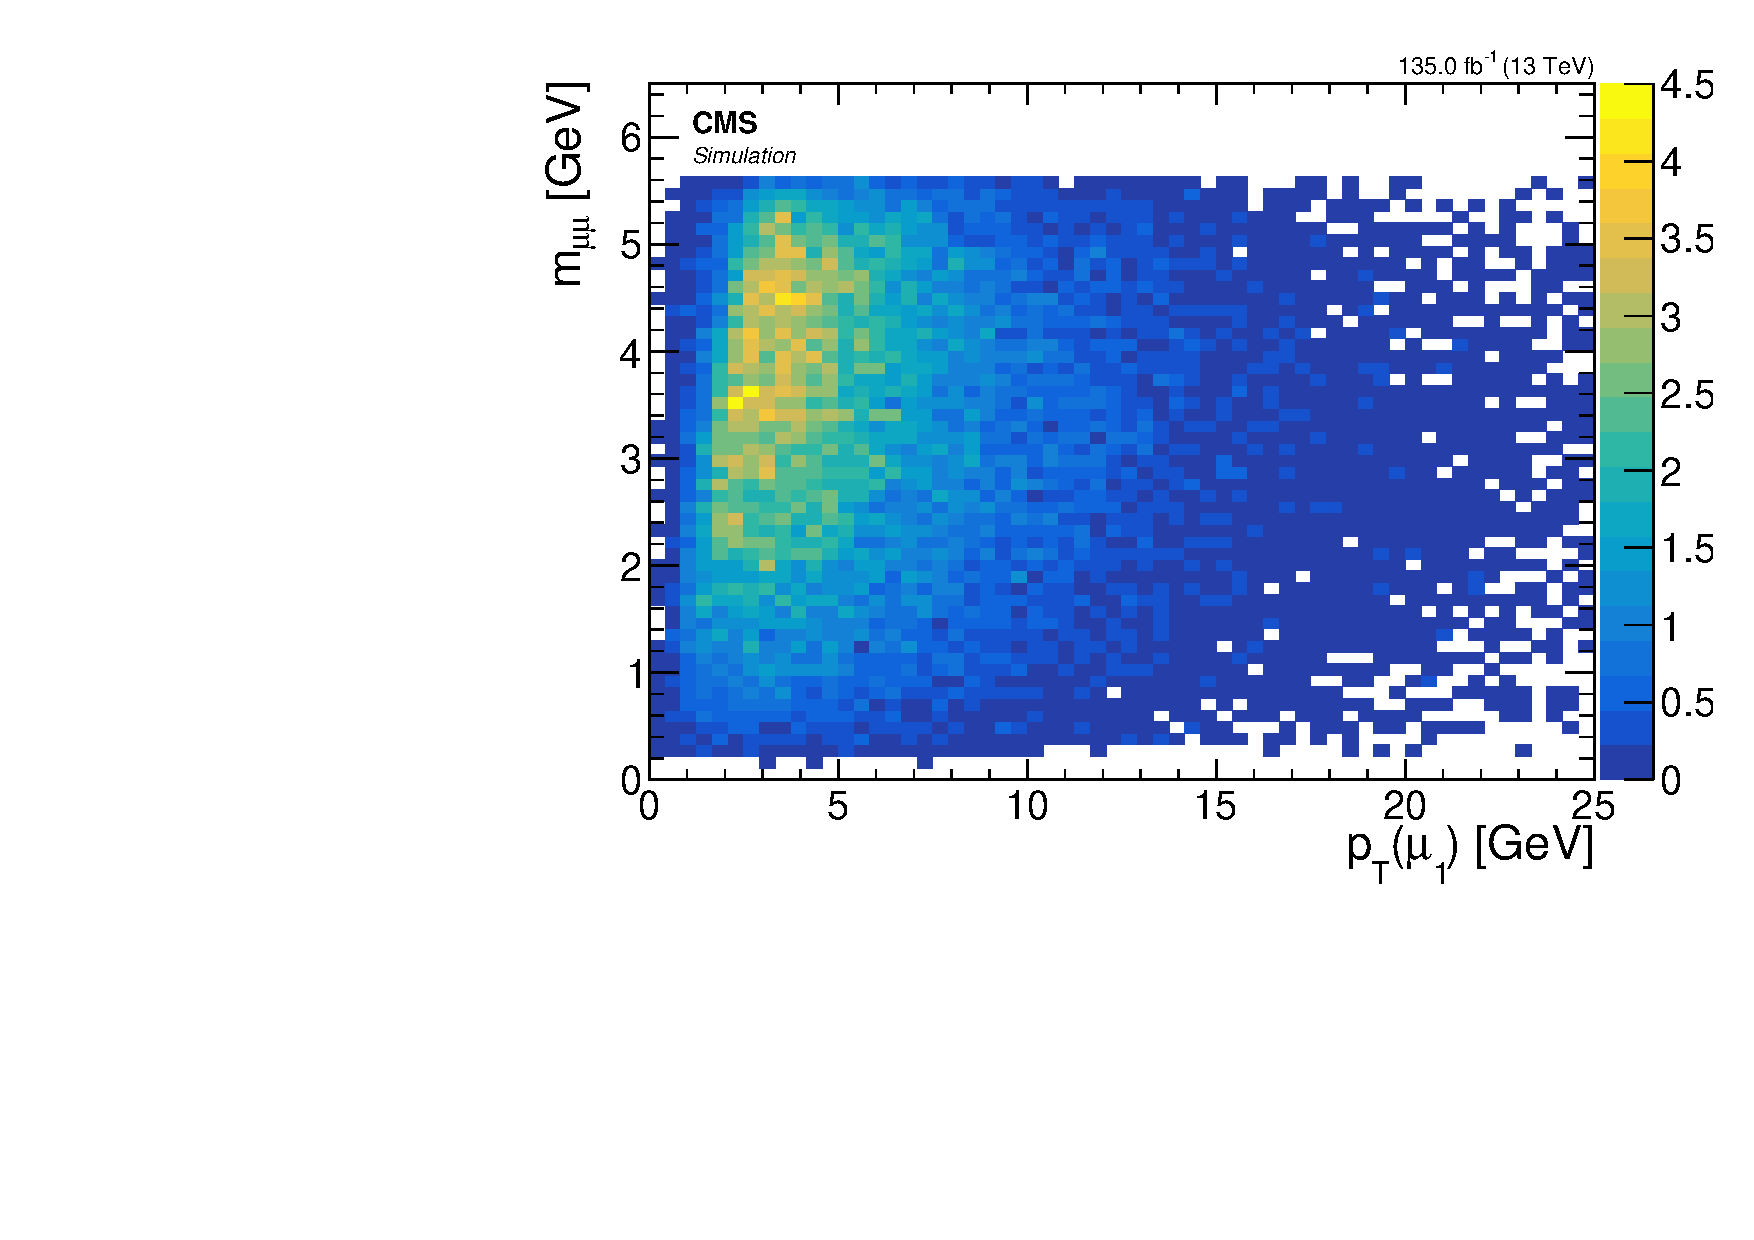
\includegraphics[width=0.48\linewidth]{plots/signal_muons_gen_delta_r_vs_pt_dm5/none_gen_invmass_vs_pt_1.pdf} \,
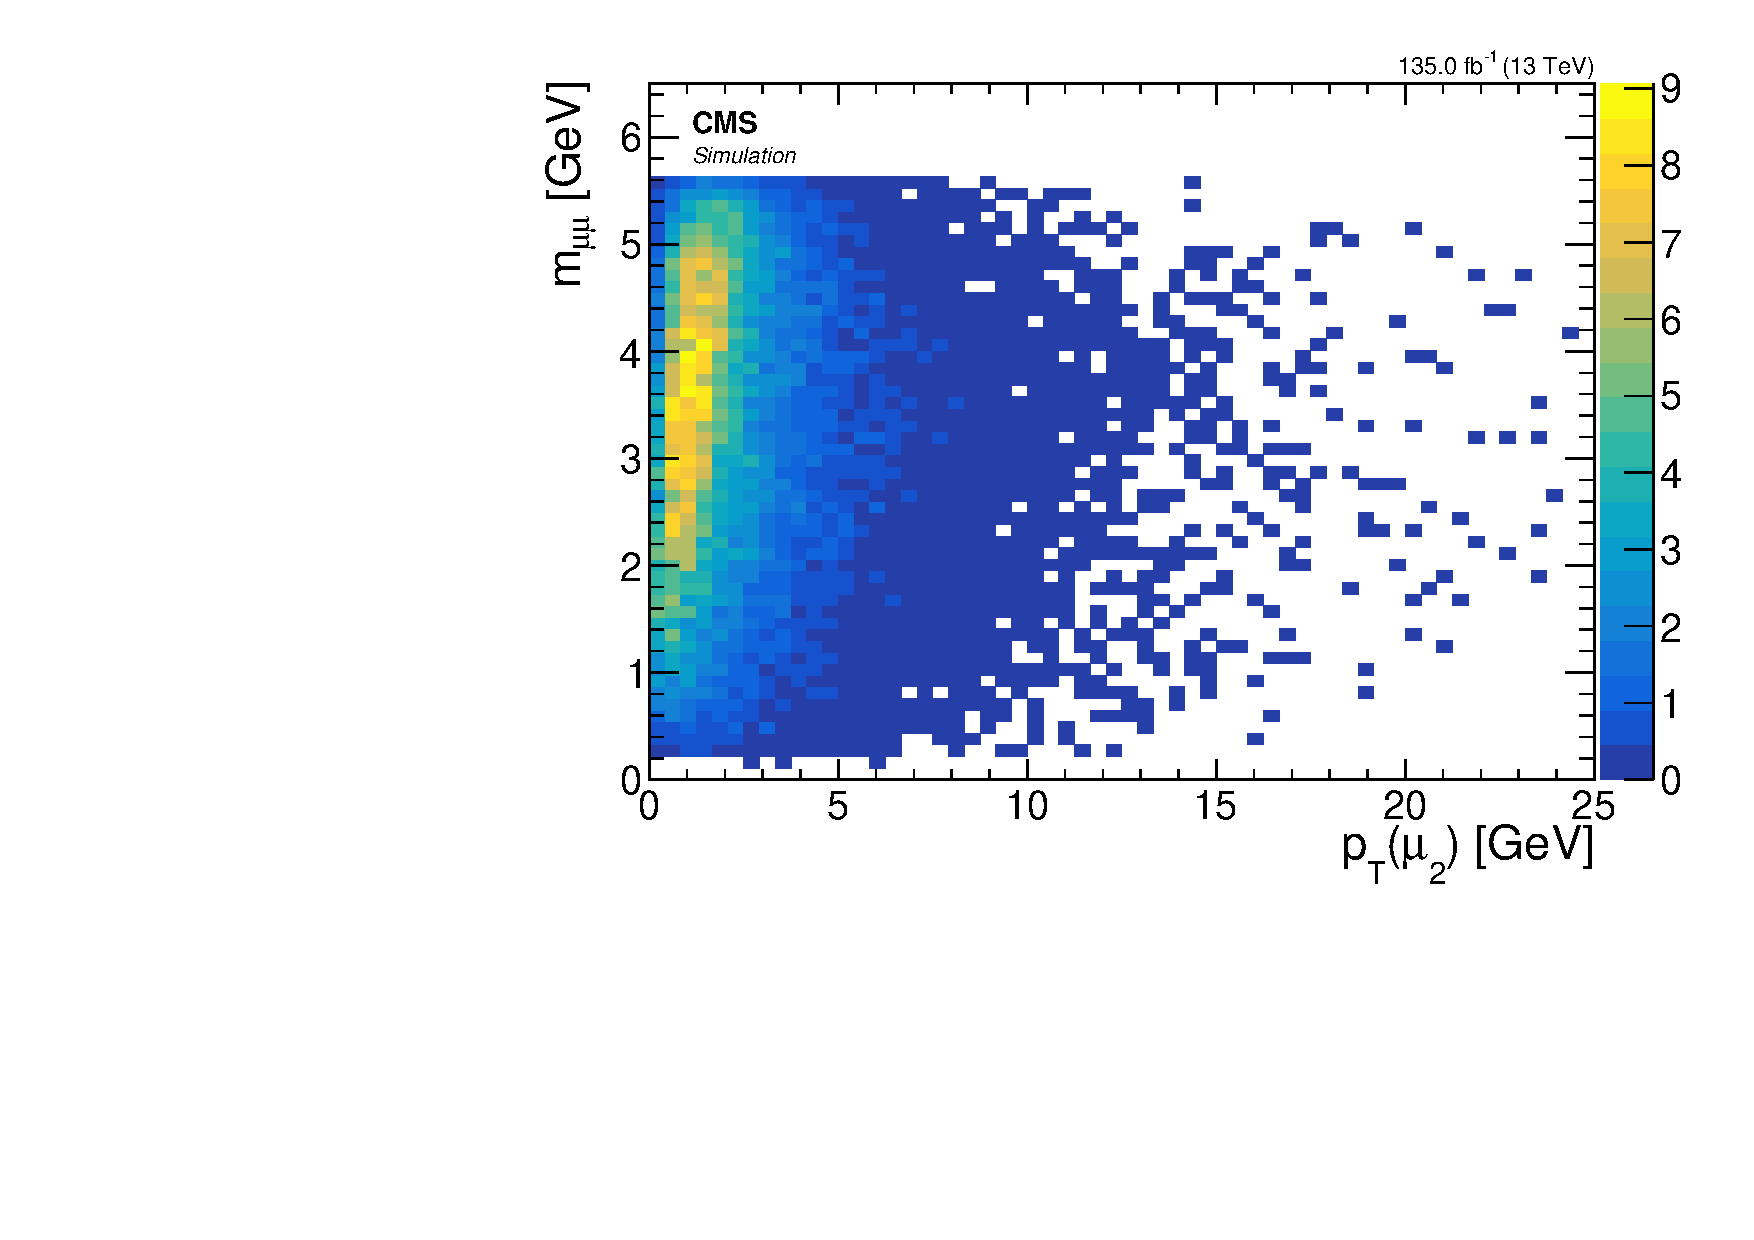
\includegraphics[width=0.48\linewidth]{plots/signal_muons_gen_delta_r_vs_pt_dm5/none_gen_invmass_vs_pt_2.pdf}  \\
\caption[Signal \mmumu \vs \pt]{ Signal \mmumu \vs \pt for leading lepton $\mu_1$ (left) and subleading lepton $\mu_2$ (right) for $\dm=1.13\GeV$ (top) and $\dm=5.63\GeV$ (bottom).}
\label{fig:signal-gen-invamass-pt}
\end{figure}

Earlier, it was established that the invariant mass distribution has an edge at \dm, and the value of \dm can be read from these plots. Another interesting feature is a lower edge in the \dm distribution at around $\sim 0.2\GeV$, which is due to each muon having a mass of around $\sim 0.1\GeV$. It is now clear that by requiring both muons to have $\pt\geq 2\GeV$, a significant portion of the signal is lost. This effect becomes particularly substantial for the low $\dm=1.13\GeV$ (top row). The magnitude of this effect is quantified by a cutflow, shown in Table~\ref{tab:gen-muon-pt-dr-efficiency}, where each row represents a cut, and its efficiency is calculated by dividing the number of events passing the cut by the number of events in the previous line. The first line the number of events with exactly 2 muons at the generator level with at least one jet with $\pt \geq 30\GeV$ and $\abs{\eta}<2.4$. The event number is weighted to Run II luminosity of $\lumi = 135 \fbinv$.

\begin{table}[!htb]
	\centering
	\label{tab:gen-muon-pt-dr-efficiency}
		\caption{Generator level efficiency on muons selections}
		%\vspace{1mm}
			\begin{tabular}{l|cc|cc} \hline
			Cut & \multicolumn{2}{c|}{Weighted number of events} & \multicolumn{2}{c}{Efficiency} \\ \hline
			
			 & $\dm=1.13\GeV$ & $\dm=5.63\GeV$ & $\dm=1.13\GeV$ & $\dm=5.63\GeV$ \\
			Baseline & 1710.7 & 1743.9 & - & -\\
			$\pt\geq 2\GeV$ & 24.7 & 724.9 & 0.015 & 0.41\\
			\gls{sos} orthogonality & 24.7 & 490.6 & 1 & 0.68 \\ \hline
			\end{tabular}
\end{table}

Table~\ref{tab:gen-muon-pt-dr-efficiency} shows that for the low $\dm$ of $1.13\GeV$, the acceptance of the signal is significantly reduced by the $\pt\geq 2\GeV$ cut, with only $1.5\%$ of the signal remaining. In contrast, the orthogonality condition of requiring $\pt\left(\mu_2\right)\leq~3.5\GeV\text{ or }\drll\leq 0.3$ does not affect it any further. The situation is different for the high \dm of $5.63\GeV$, where the \pt cut rejects more than half of the signal and the \gls{sos} orthogonality condition rejects an additional two thirds.

It has been established that the \pt thresholds affect the \mll distribution due to the relationship between the two variables. Next, it is investigated how the reconstruction discussed in Section~\ref{sec:muon-eta-pt} impacts the \mmumu distribution. The distributions of the reconstructed \mmumu can be seen in Figure~\ref{fig:reco-signal-invamass}. Comparing these distributions to to the two right plots in Figure~\ref{fig:signal-generator-mll} not only are fewer events surviving the reconstruction, but also some \dm model points are peaking between $1 \GeV$ to $2 \GeV$ with the \gls{sos} orthogonality condition applied.

\begin{figure}[!htb]
\centering
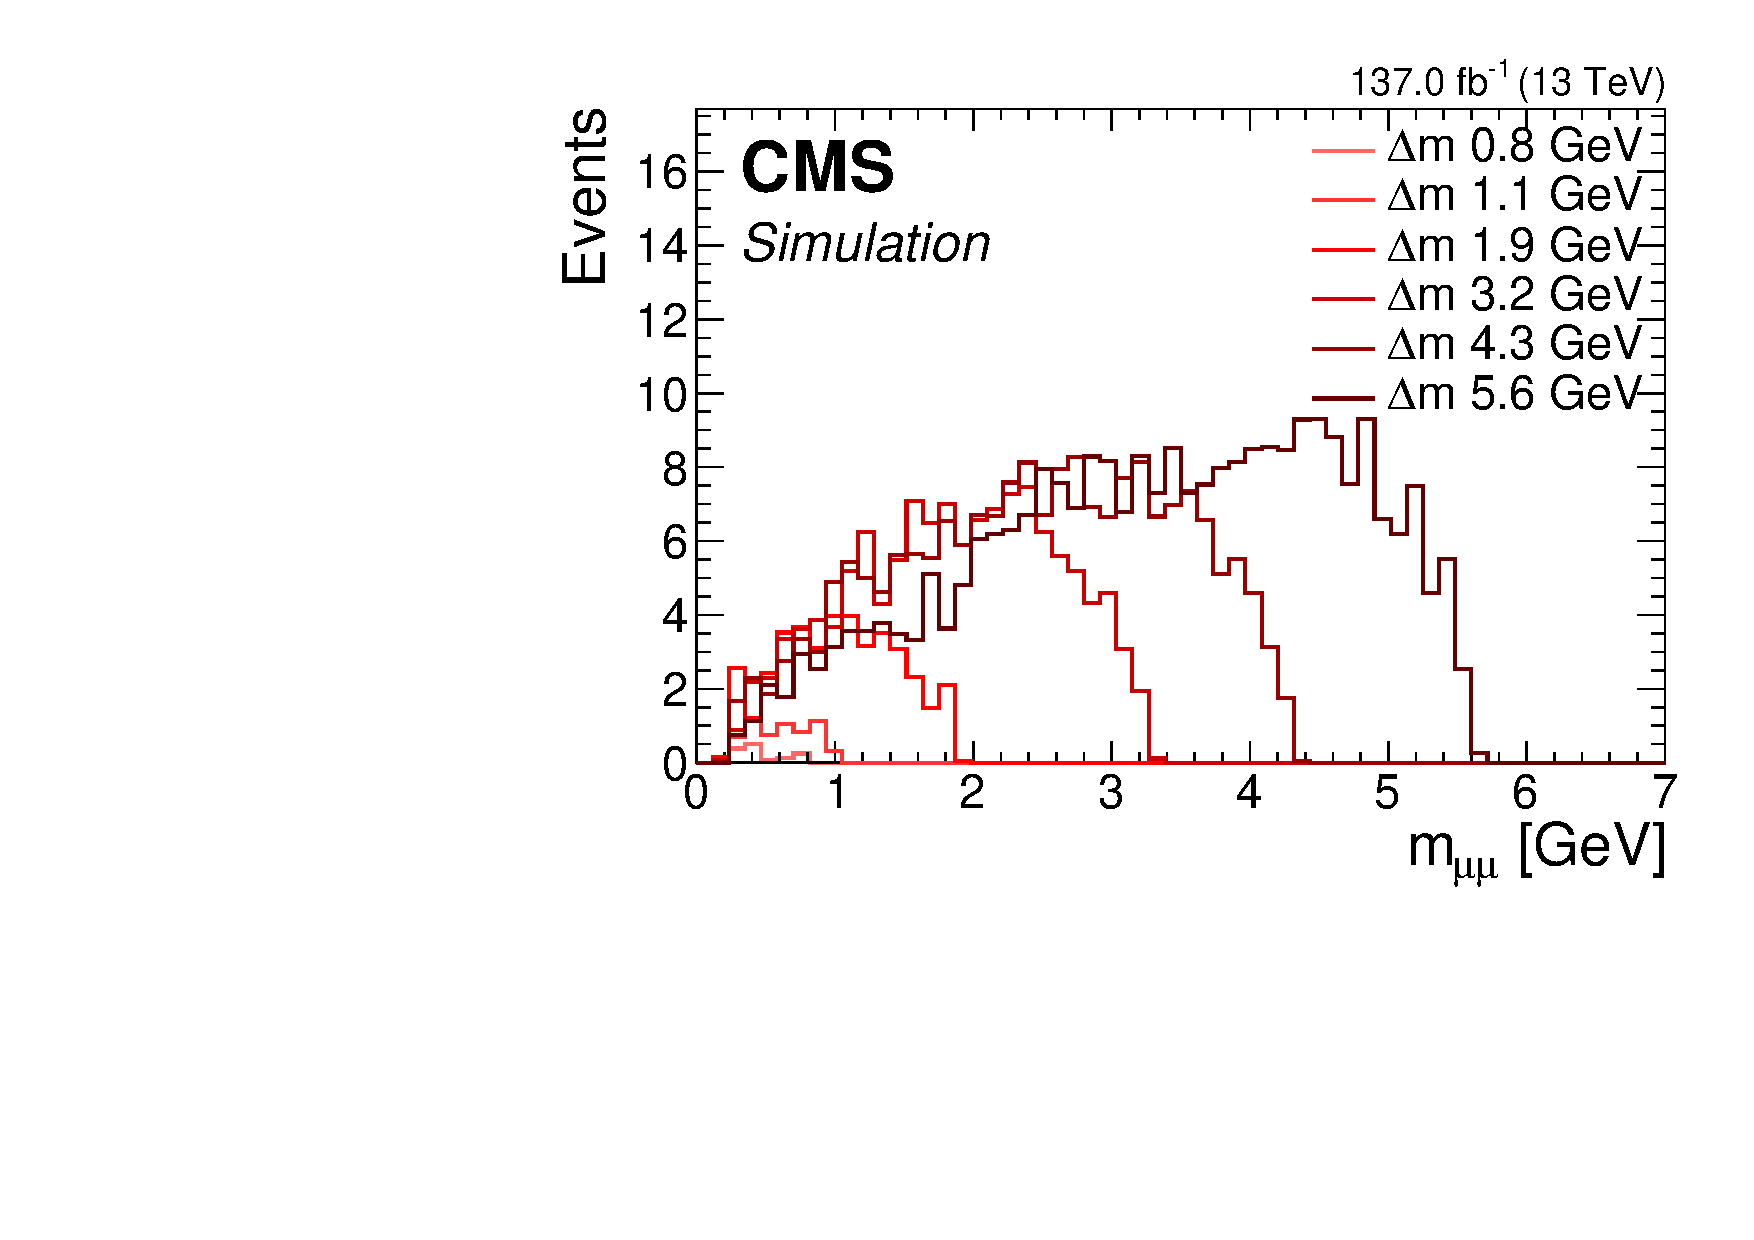
\includegraphics[width=0.48\linewidth]{plots/signal_muons/none_invMassCorrJetNoMultIso10Dr0.6.pdf} \,
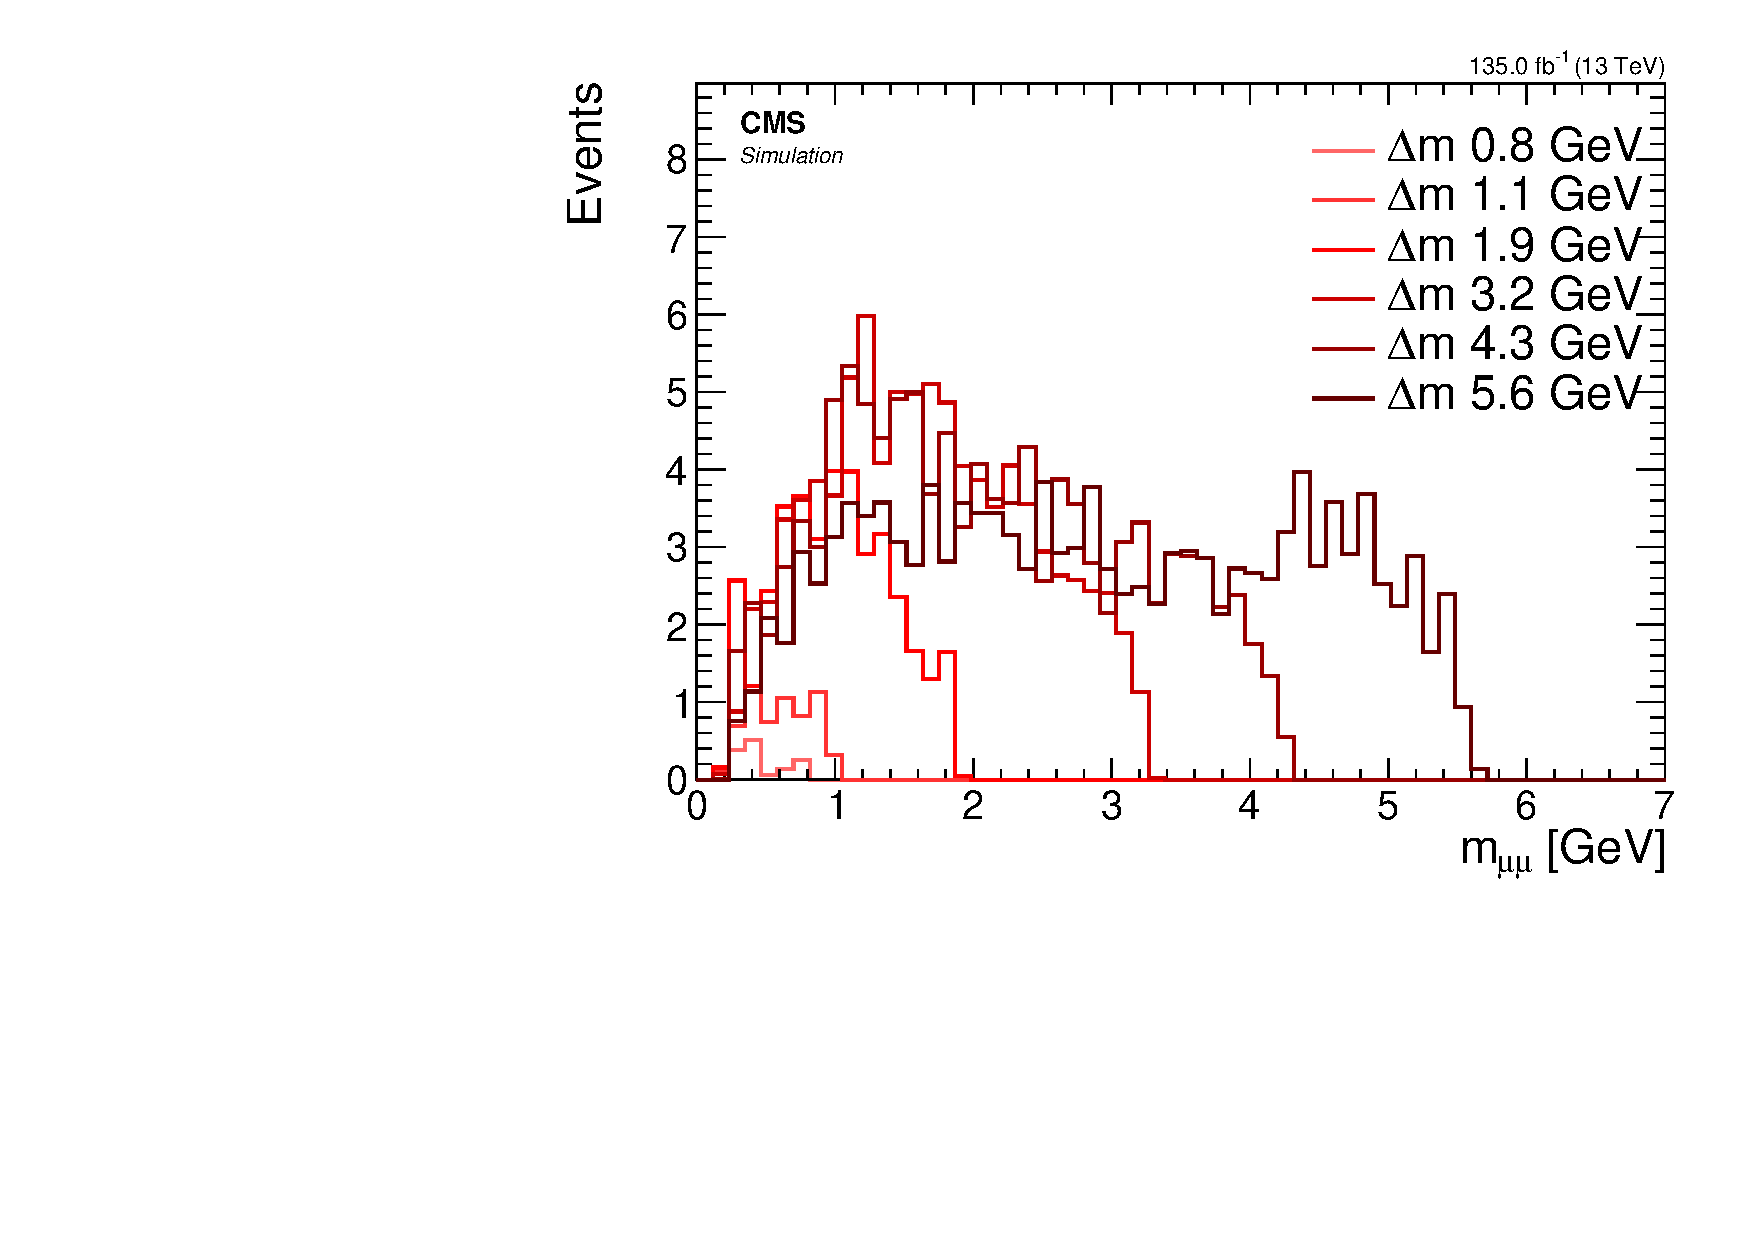
\includegraphics[width=0.48\linewidth]{plots/signal_muons/none_invMassCorrJetNoMultIso10Dr0.6_orth.pdf}  \\
\caption[Distributions of reconstructed \mmumu in signal events]{ Distributions of reconstructed \mmumu in signal events with analysis selection (left) and the additional \gls{sos} orthogonality condition (right).}
\label{fig:reco-signal-invamass}
\end{figure}

\subsubsection{Lepton separation \gls{dr}}
\label{sec:lepton-dr}

The lepton separation is defined by the equation $\DR=\sqrt{\left(\deta\right)^2+\left(\dphi\right)^2}$, where \gls{eta} represents the pseudorapidity and \gls{phi} is the azimuthal angle measured in radians. The value of \gls{dr} is significant in this analysis because the produced leptons tend to be located in close proximity to each other and therefore are not easily isolated according to standard definitions. Special attention is given to ensuring that the collimated nature of the leptons can be used to differentiate signal leptons from the non-isolated leptons in the \gls{sm} background. It is worth noting that, for the purposes of orthogonality, the requirement of $\drll > 0.3$ utilized in previous \gls{sos} analyses~\citep{sos} is reverted.

Similar to the invariant mass discussed in Section~\ref{sec:gen-invariant-mass}, we examine the distributions of \gls{dr} for various \dm options with different cuts applied to observe their effect. The left plot of Figure~\ref{fig:signal-generator-dr} shows that roughly the same number of events are produced for all \dm model points. However, when applying a cut of $\pt\left(\mu\right)>2\GeV$, a hierarchy of \dm points emerges, with fewer events as \dm becomes smaller (middle plot). The spike on the right plot is due to the \gls{sos} orthogonality condition, which requires $\drll\leq 0.3$ as one of two conditions that must be satisfied.

\begin{figure}[!htb]
\centering
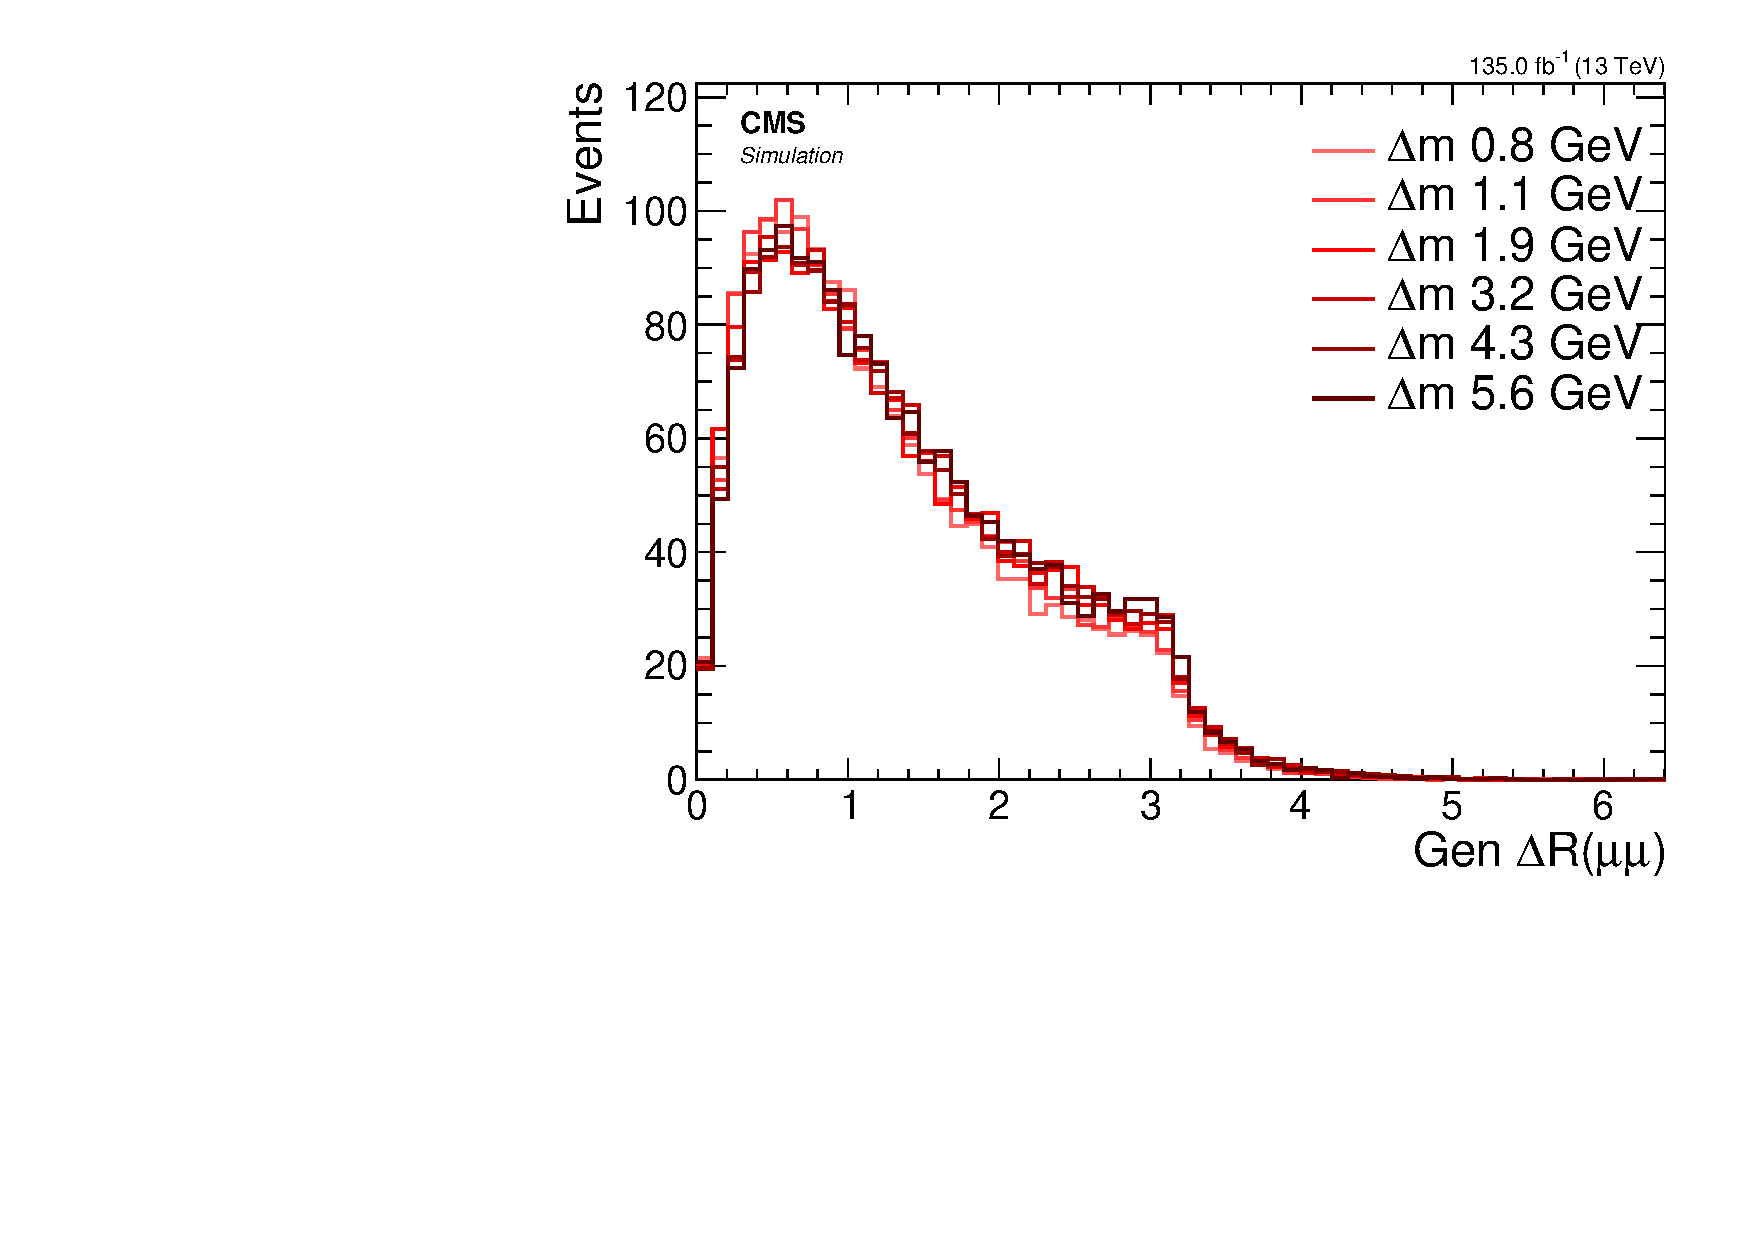
\includegraphics[width=0.32\linewidth]{plots/signal_muons_gen/none_gen_deltaR.pdf} \,
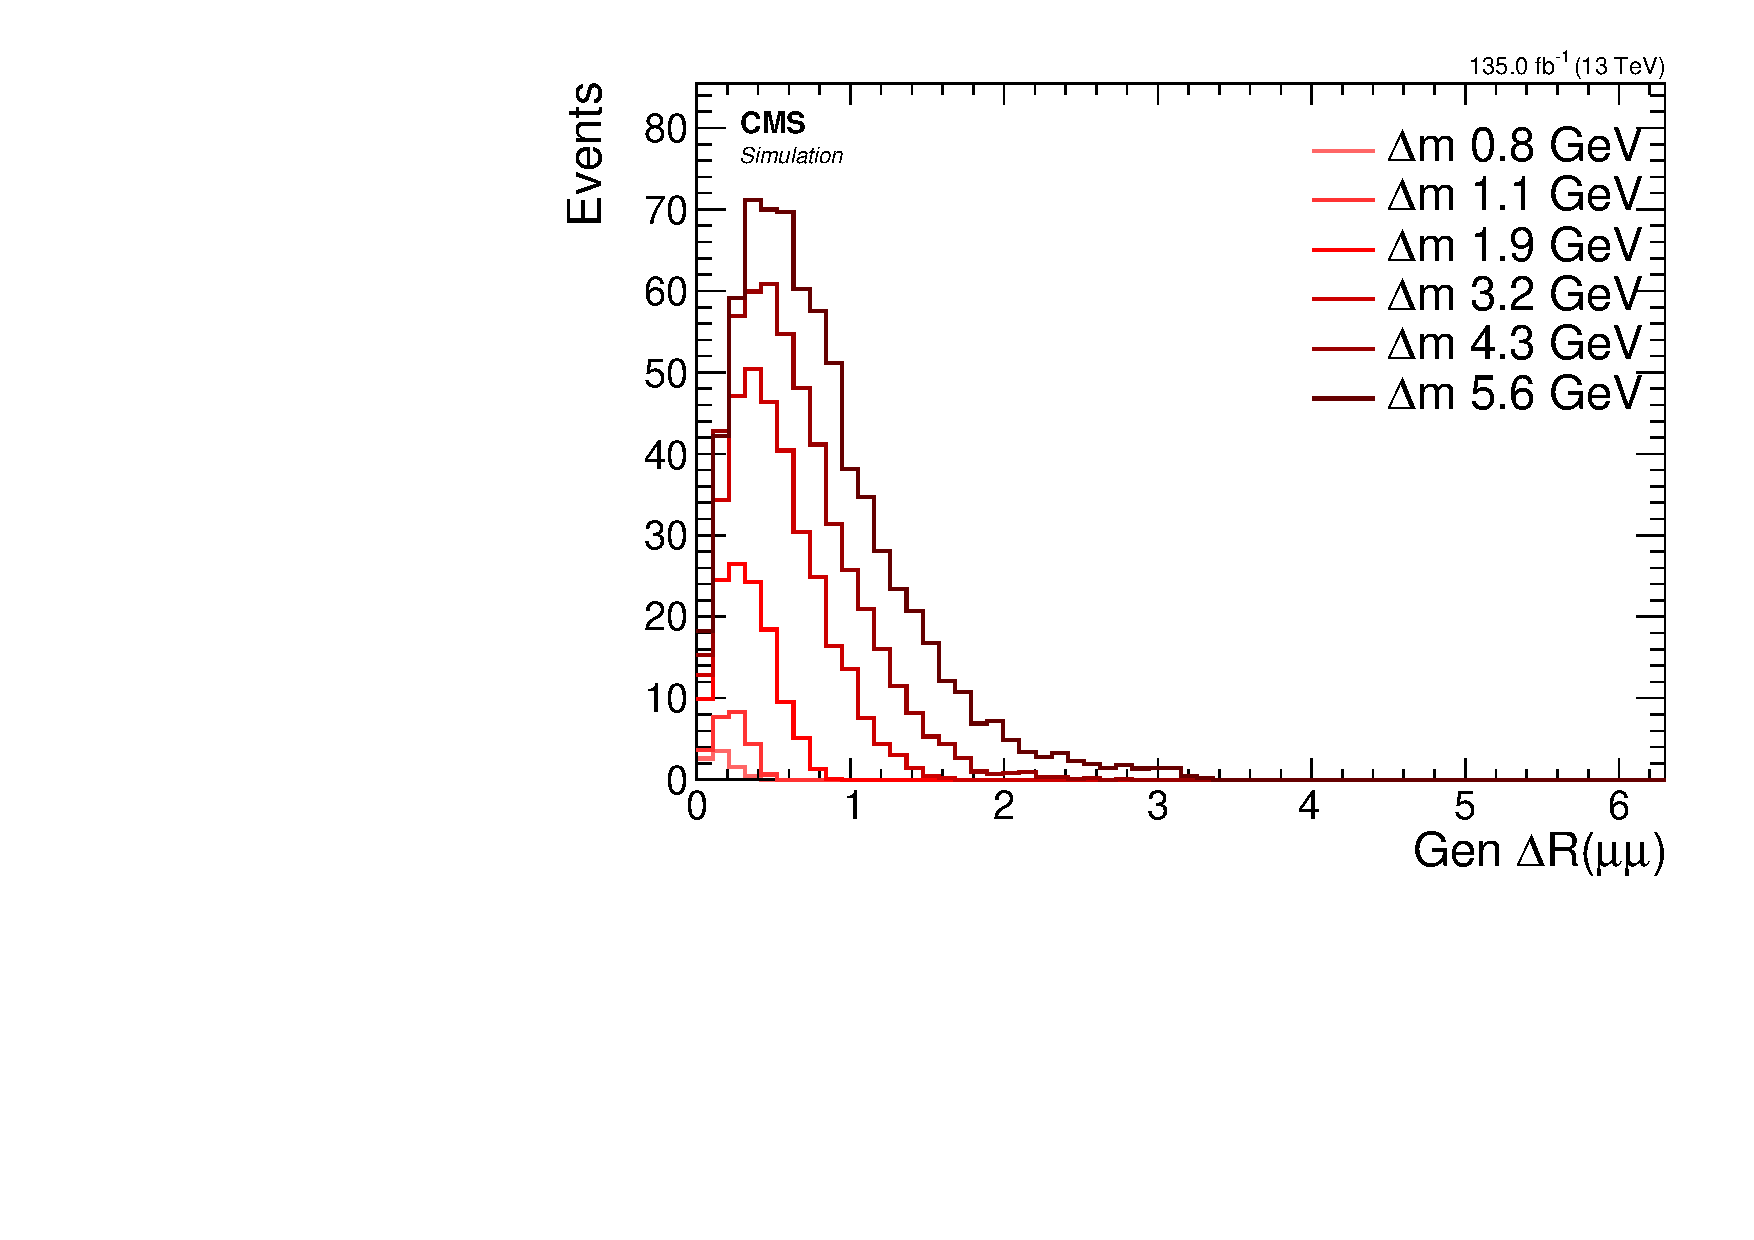
\includegraphics[width=0.32\linewidth]{plots/signal_muons_gen/none_gen_deltaR_cut.pdf}  \,
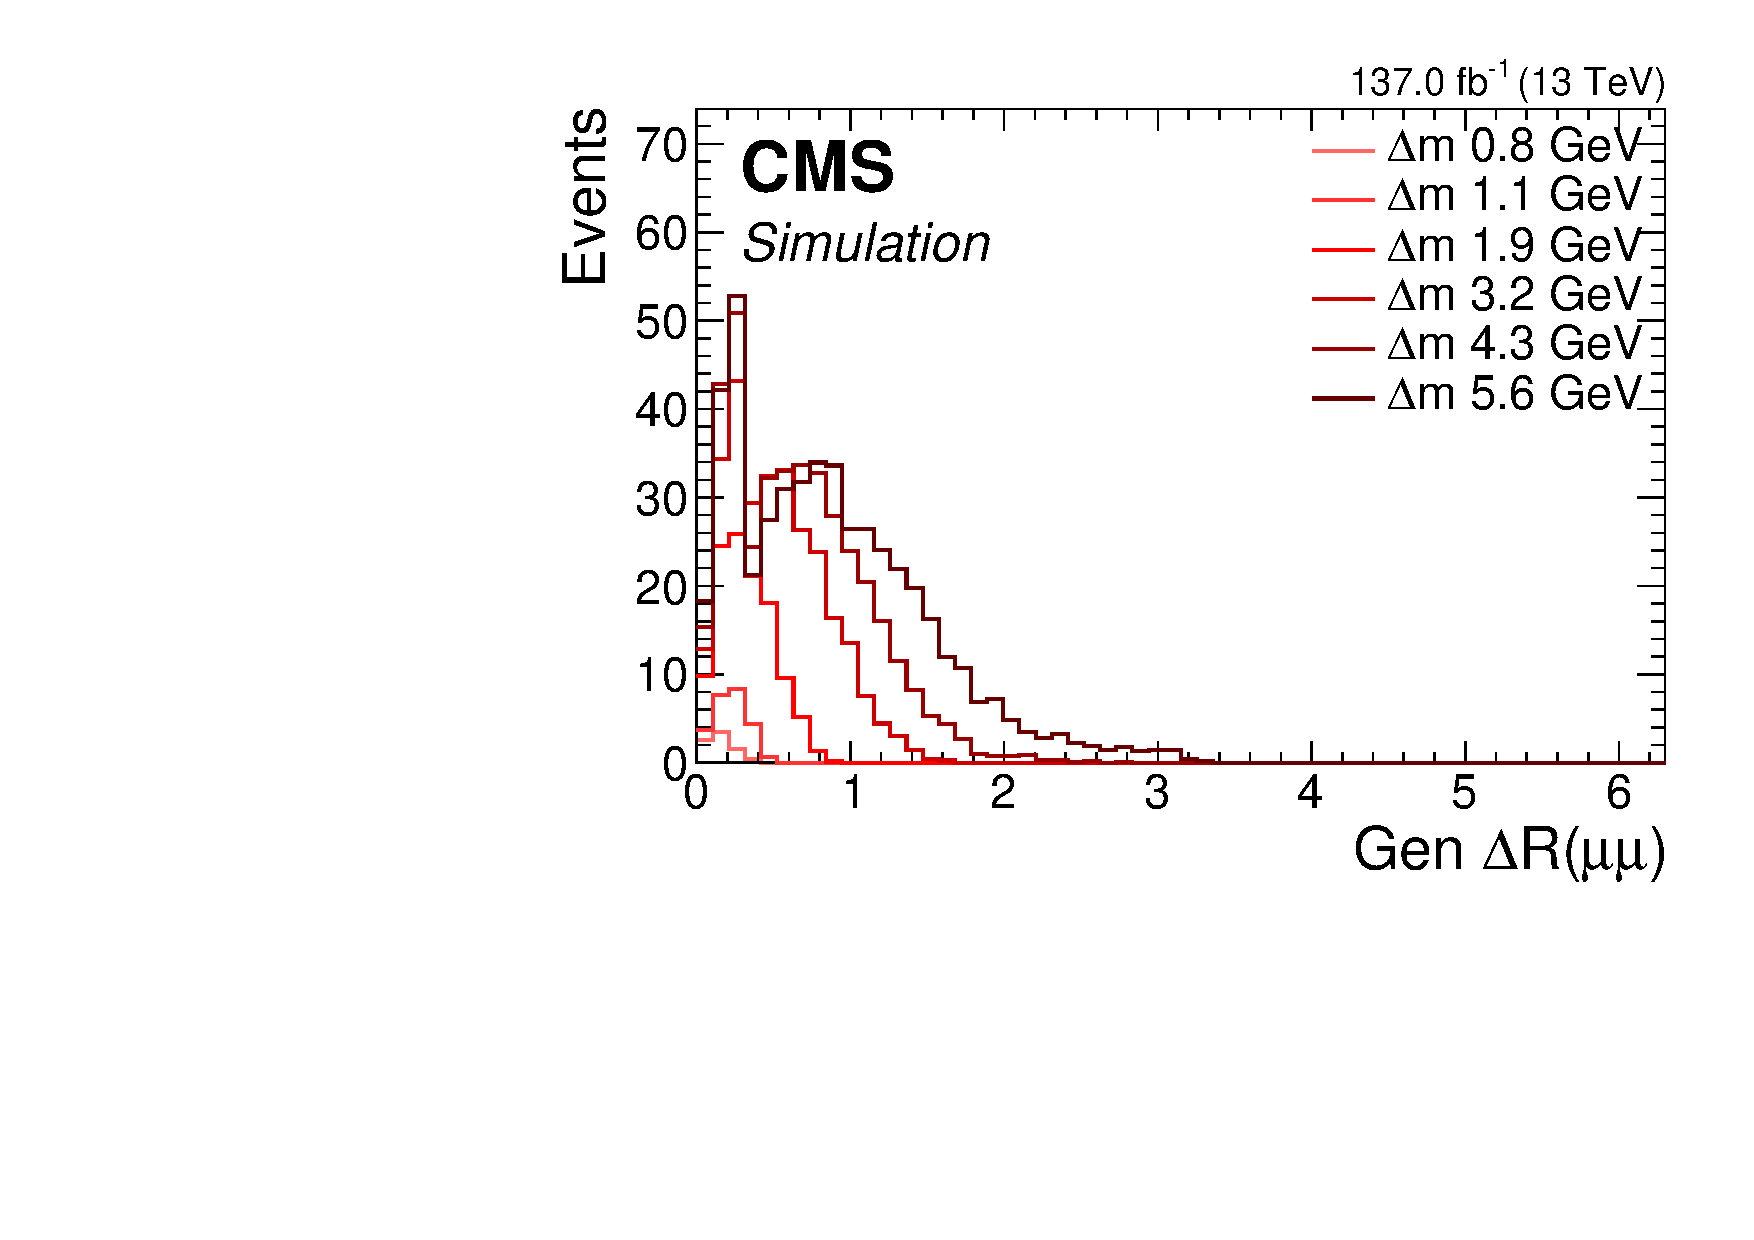
\includegraphics[width=0.32\linewidth]{plots/signal_muons_gen/none_gen_deltaR_orth.pdf} \\
\caption[Signal generator level \DR distributions]{ Signal generator level \gls{dr} distributions with no cuts (left), with $\pt\left(\mu_i\right)>2\GeV,\,i=1,2$ (middle) and with \gls{sos} orthogonality condition $\pt\left(\mu_i\right)>2\GeV$, $\pt\left(\mu_2\right)\leq~3.5\GeV\text{ or }\DR\leq 0.3$ (right).}
\label{fig:signal-generator-dr}
\end{figure}

To understand the shaping and hierarchy formation due to the \gls{pt} cut, the \pt of the muons is plotted \vs \drll in Figure~\ref{fig:signal-gen-dr-pt}. Requiring $\pt\left(\mu_2\right)\geq 2\GeV$ for $\dm=1.13\GeV$ limits the range of \drmm to less than $0.4$, while leaving a large range exceeding 3 for the $\dm=5.63\GeV$ model point. To gain access and sensitivity to the low \dm model points, allowing small \drll values, less than 0.3 is necessary, even before considering the reconstruction efficiency of the leptons. In the next sections, the study of reconstructed leptons and the isolation criteria will enable the retention of signal points with highly-columnated lepton pairs, as further explored in Section~\ref{sec:isolation}.

\begin{figure}[!htb]
\centering
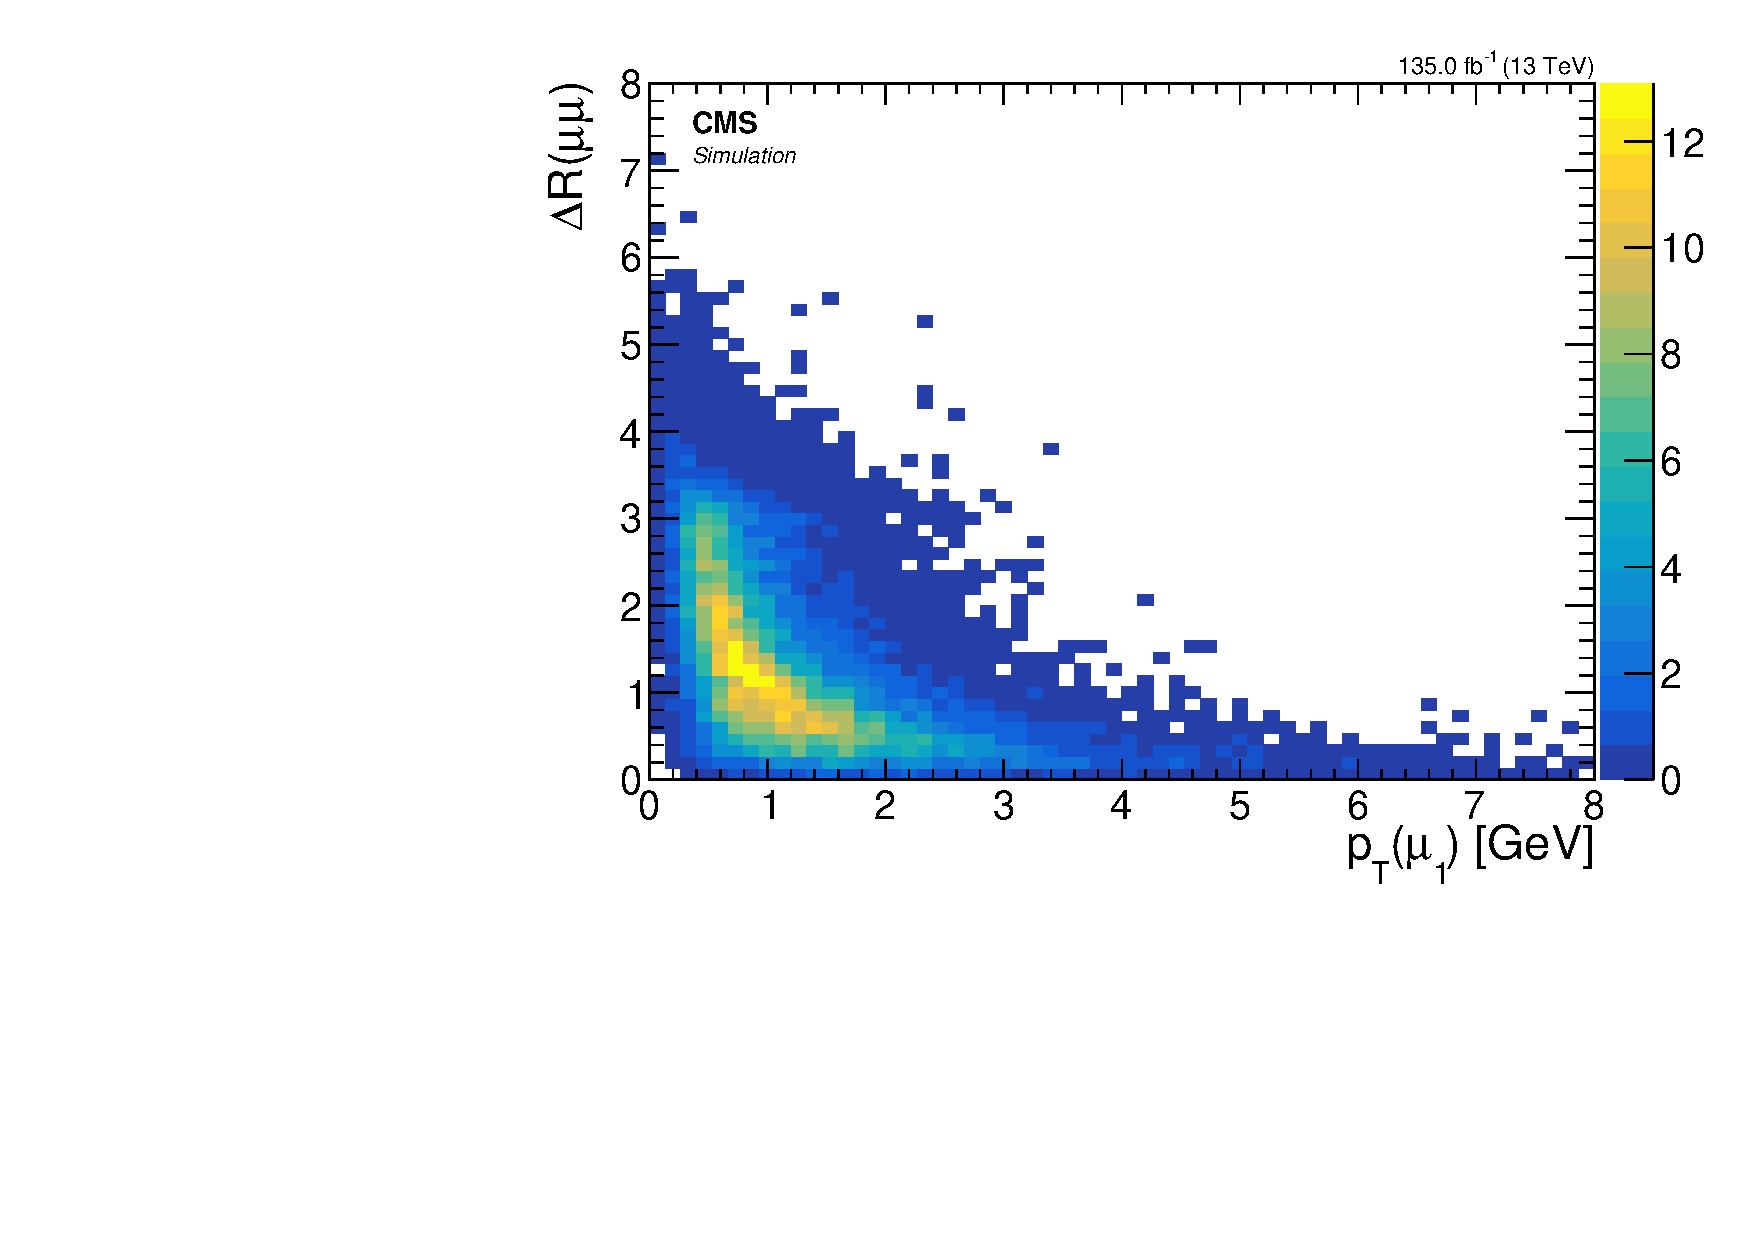
\includegraphics[width=0.48\linewidth]{plots/signal_muons_gen_delta_r_vs_pt/none_gen_delta_r_vs_pt_1.pdf} \,
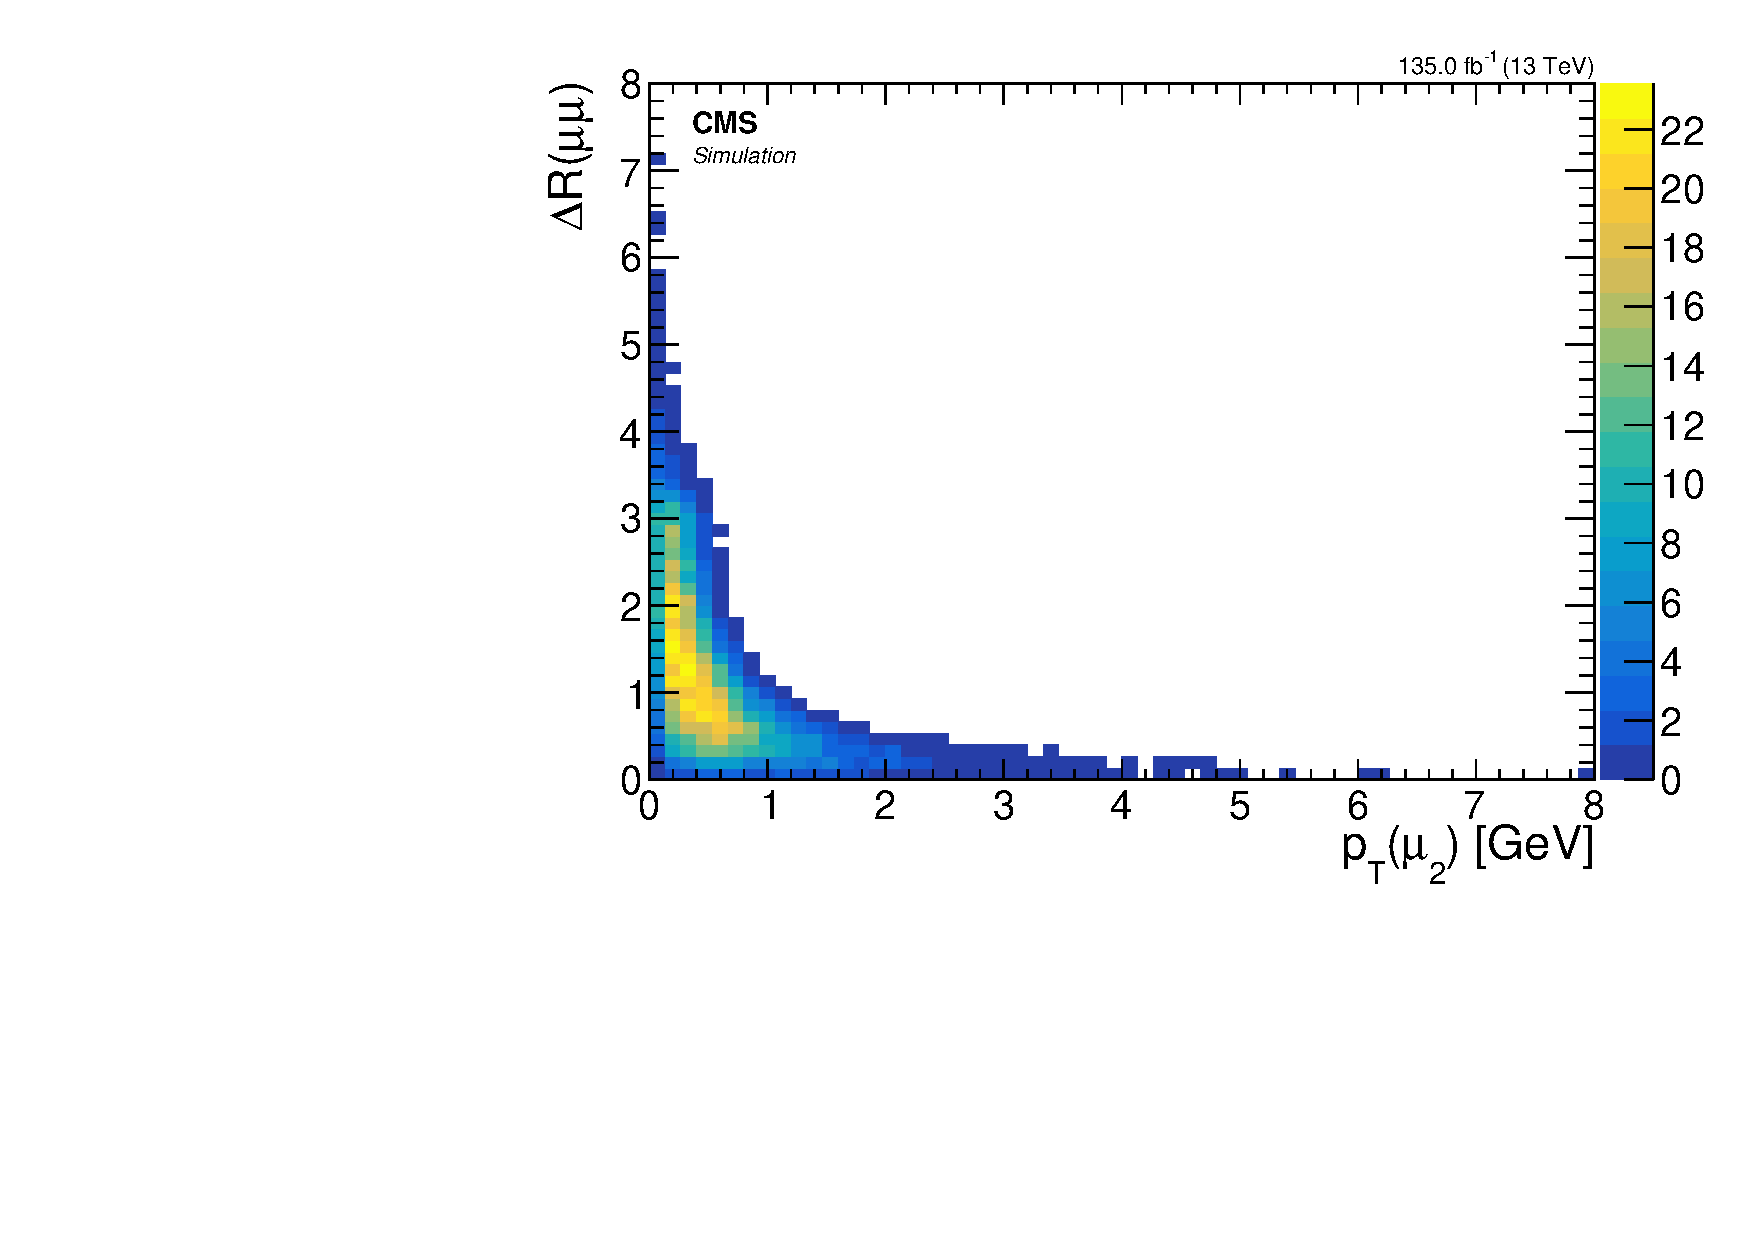
\includegraphics[width=0.48\linewidth]{plots/signal_muons_gen_delta_r_vs_pt/none_gen_delta_r_vs_pt_2.pdf}  \\
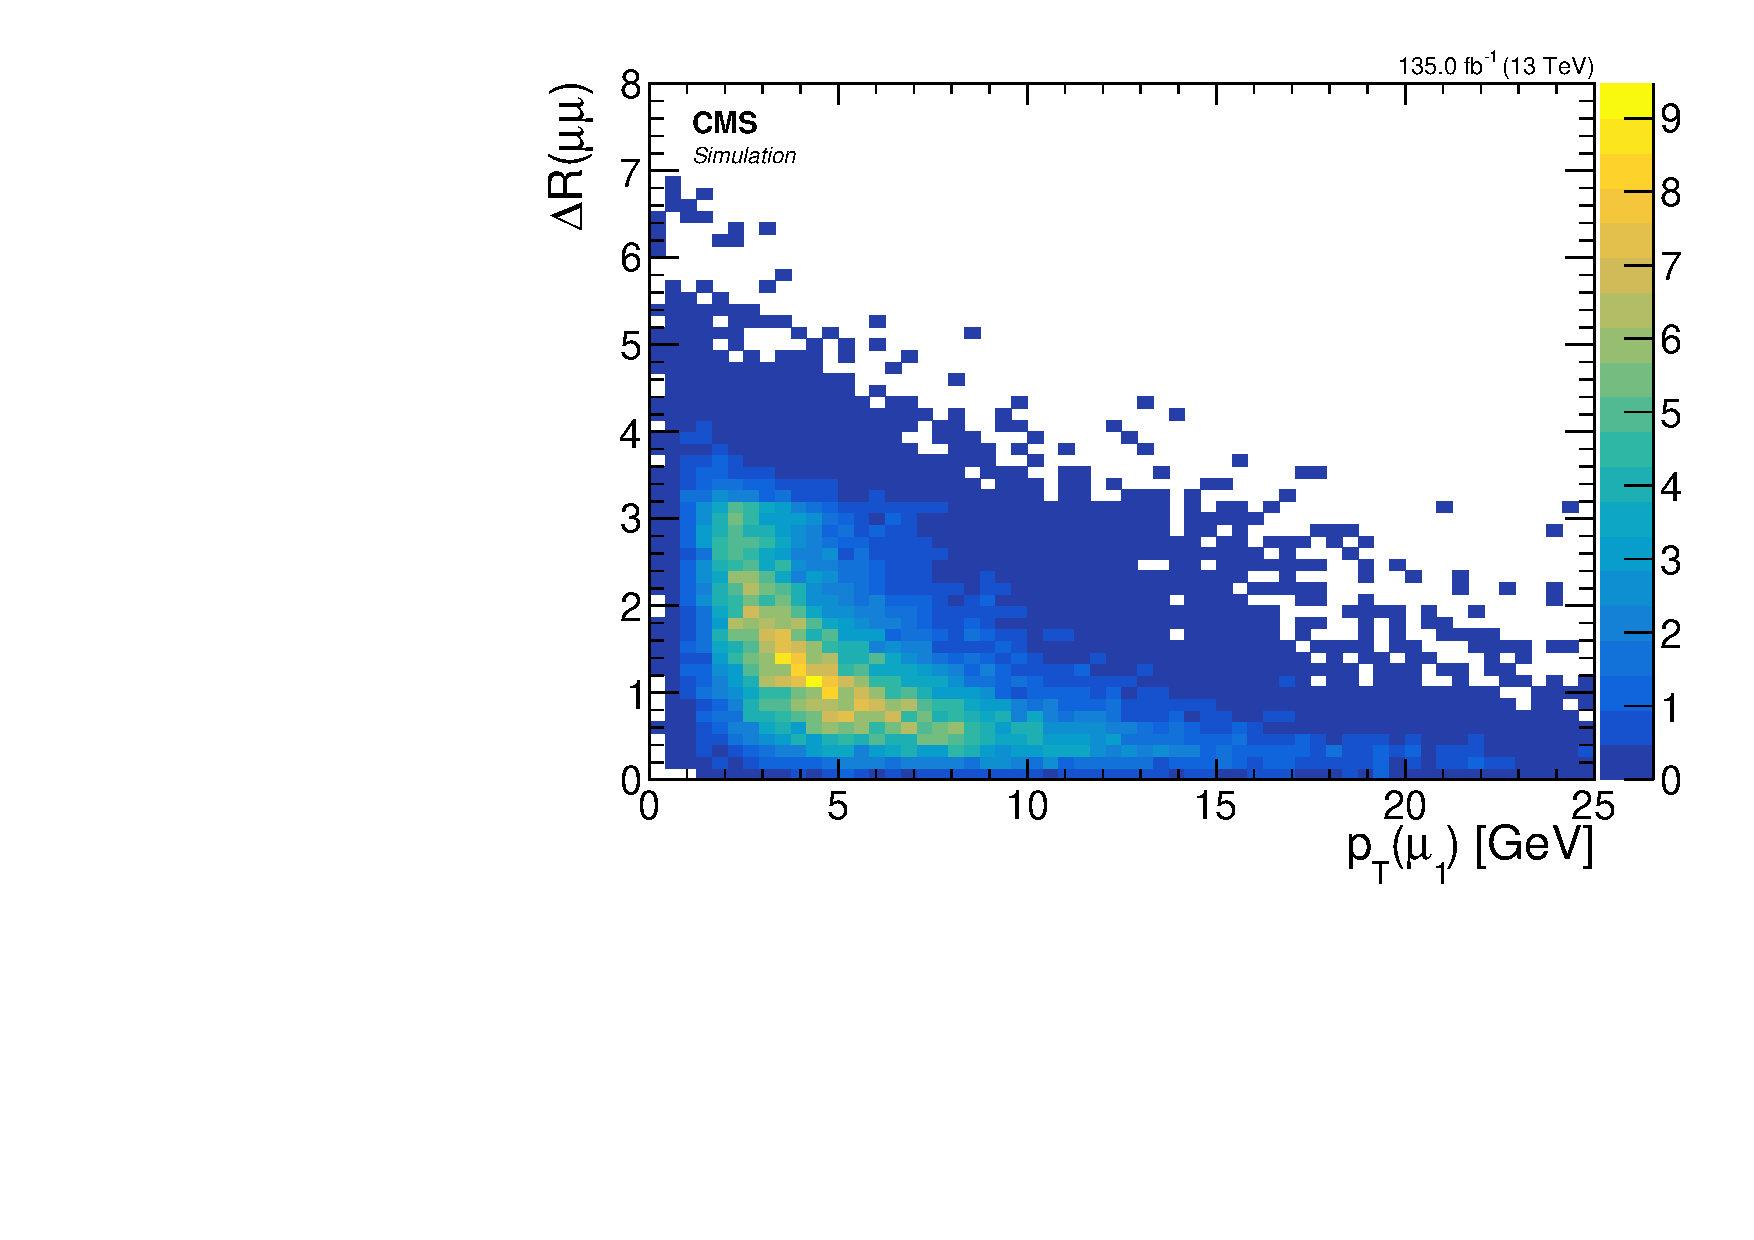
\includegraphics[width=0.48\linewidth]{plots/signal_muons_gen_delta_r_vs_pt_dm5/none_gen_delta_r_vs_pt_1.pdf} \,
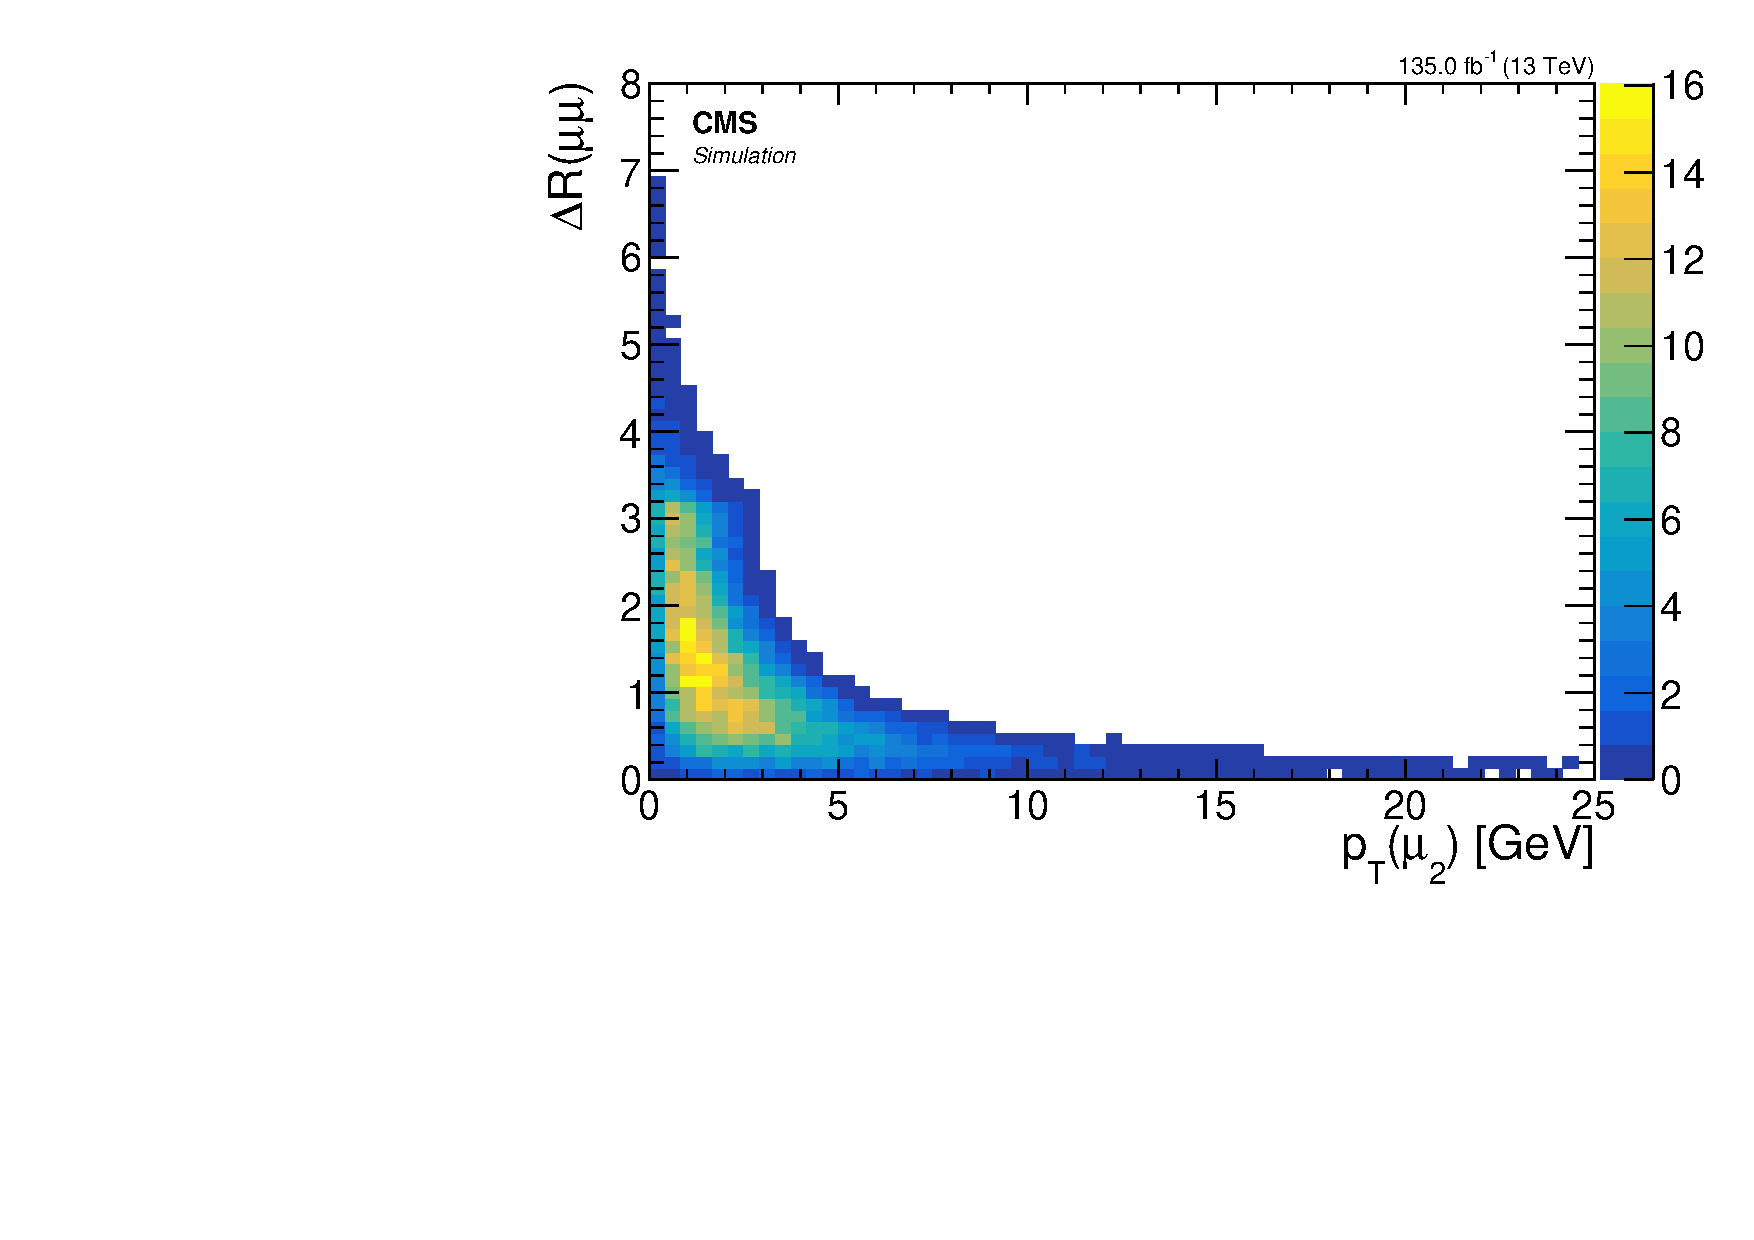
\includegraphics[width=0.48\linewidth]{plots/signal_muons_gen_delta_r_vs_pt_dm5/none_gen_delta_r_vs_pt_2.pdf}  \\
\caption[Event distributions in the plan of \drmm \vs \pt for signal models]{ Event distributions in the plan of \drmm \vs \pt for leading lepton $\mu_1$ (left) and subleading lepton $\mu_2$ (right) for signal models with $\dm=1.13\GeV$ (top) and $\dm=5.63\GeV$ (bottom).}
\label{fig:signal-gen-dr-pt}
\end{figure}

As seen in Section~\ref{sec:gen-invariant-mass} for \mmumu, reconstruction has an effect on both the shape and overall count of events. The effects on the \drmm distributions are investigated in Figure~\ref{fig:reco-signal-dr}.

\begin{figure}[!htb]
\centering
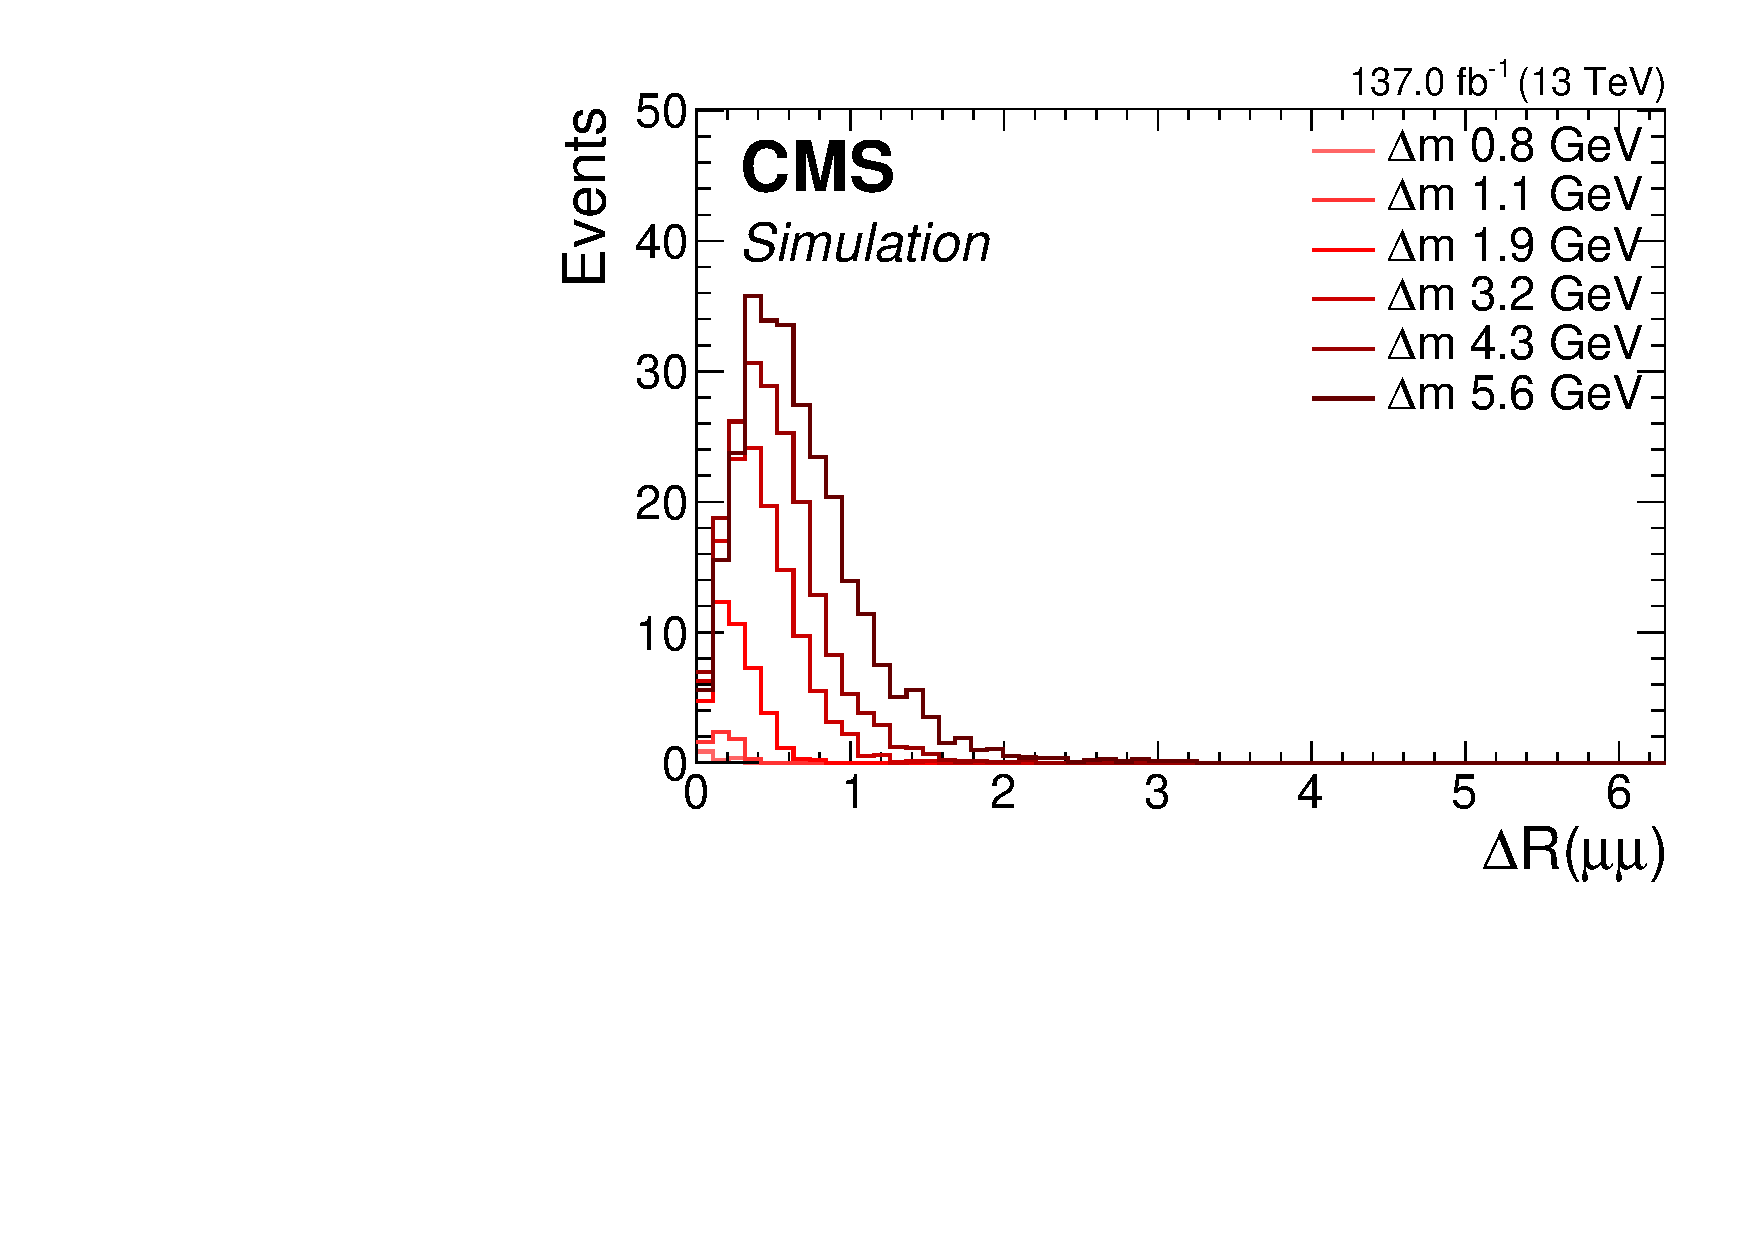
\includegraphics[width=0.48\linewidth]{plots/signal_muons/none_deltaRCorrJetNoMultIso10Dr0.6.pdf} \,
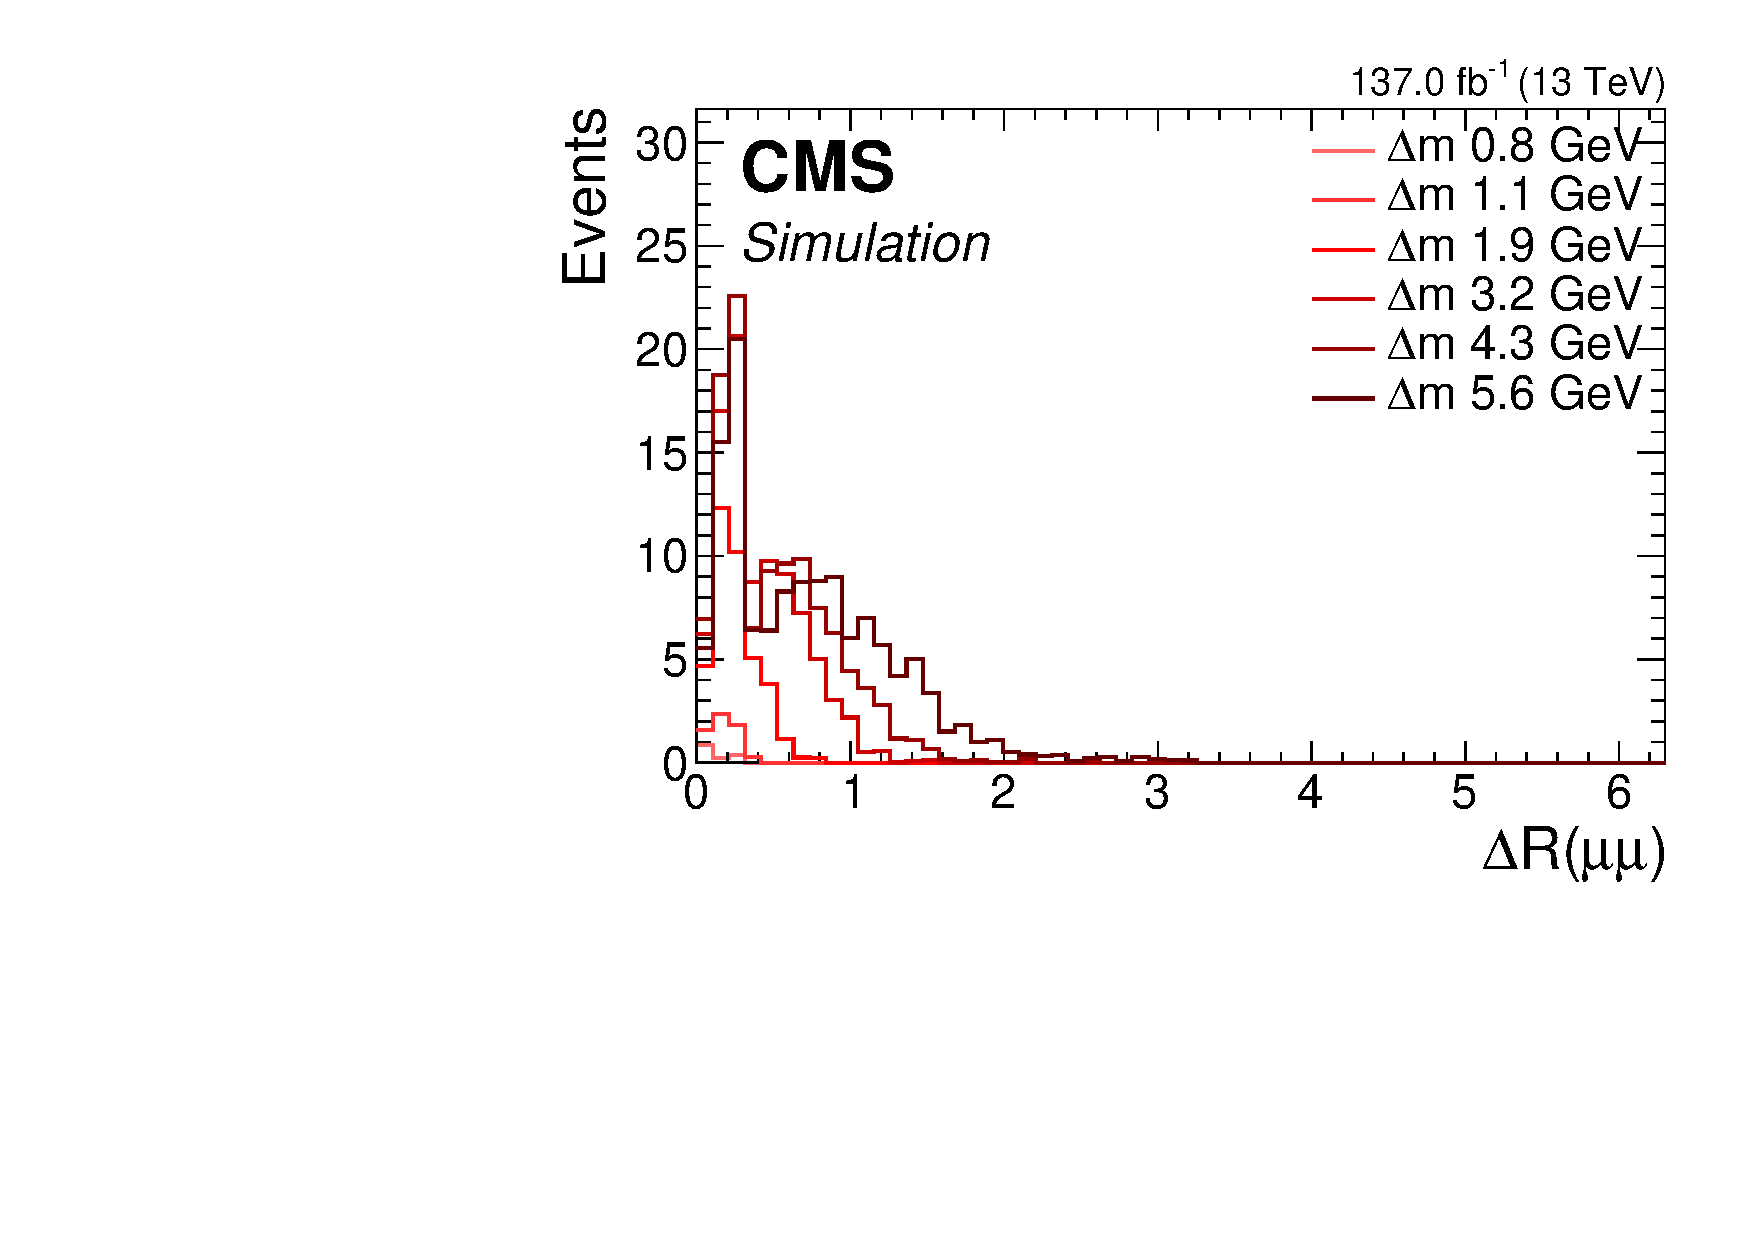
\includegraphics[width=0.48\linewidth]{plots/signal_muons/none_deltaRCorrJetNoMultIso10Dr0.6_orth.pdf}  \\
\caption[Distributions of the reconstructed \drmm in signal events]{ Distributions of the reconstructed \drmm with preselection applied (left) and the additional \gls{sos} orthogonality condition (right).}
\label{fig:reco-signal-dr}
\end{figure}

Comparing Figure~\ref{fig:reco-signal-dr} and Figure~\ref{fig:signal-generator-dr}, the main effect of the reconstruction on the \drmm is the overall normalization, which is due to reconstruction efficiency.

\clearpage 
\subsection{Main drivers of sensitivity}

The above studies reveal the main drivers of the sensitivity to different model points of this analysis, and may inform future analysis strategies that expand on the current work. This section has not explicitly included \gls{sm} background in the plots, making it hard to conclude what effects changing the cuts to \MET or other event level observables might have. However, it is very clear from examining the dilepton kinematics that for low \dm model points, regions with low \pt and \gls{dr} contain the bulk of the signal events. Another driver of the sensitivity at all \dm model points is the luminosity, since the production cross section drops as a function of the higgsino mass parameter $\mu$.

The next sections will explore how to lower the threshold on the muon transverse momentum and deal with collimated leptons that might pose a challenge in regards to the isolation criterion.
